\documentclass[12pt, a4paper]{article}

% ============================================================================
% PAQUETES
% ============================================================================
\usepackage[utf8]{inputenc}
\usepackage[T1]{fontenc}
\usepackage[spanish, es-tabla]{babel}
\usepackage{geometry}
\geometry{margin=2.5cm}
\usepackage{parskip}
\usepackage{listings}
\usepackage{xcolor}
\usepackage{amsmath, amssymb}
\usepackage{booktabs}
\usepackage{array}
\usepackage{enumitem}
\usepackage{fancyhdr}
\usepackage{titlesec}
\usepackage{float}
\usepackage{graphicx}
\usepackage{hyperref}

% Fuentes de alta calidad académica (Monocromáticas y elegantes)
\usepackage{mathpazo}
\usepackage[scaled=0.92]{helvet}
\usepackage{courier}

% ============================================================================
% TIKZ Y LIBRERIAS
% ============================================================================
\usepackage{tikz}
\usetikzlibrary{
  positioning,
  arrows.meta,
  calc,
  decorations.pathreplacing
}

% ============================================================================
% COLORES PERSONALIZADOS (MONOCROMÁTICOS Y PASTEL)
% ============================================================================
\definecolor{penblue}{RGB}{0, 0, 0} 
\definecolor{codebg}{RGB}{248,248,248} % Gris muy claro de fondo
\definecolor{codegreen}{gray}{0.4} % Comentarios en gris oscuro
\definecolor{codepurple}{gray}{0.1}
\definecolor{codegray}{gray}{0.5}
\definecolor{codeblue}{gray}{0.0} % Palabras clave en negro
\definecolor{pastelblue}{RGB}{230, 242, 252} % Celeste claro pastel sutil para rellenar bloques

% ============================================================================
% CONFIGURACION DE LISTINGS
% ============================================================================
\lstdefinestyle{verilogstyle}{
  language=Verilog,
  backgroundcolor=\color{codebg},
  basicstyle=\ttfamily\footnotesize,
  keywordstyle=\color{codeblue}\bfseries,
  commentstyle=\color{codegreen}\itshape,
  stringstyle=\color{codepurple},
  numberstyle=\tiny\color{codegray},
  numbers=left,
  numbersep=8pt,
  frame=leftline, 
  framerule=2pt,
  rulecolor=\color{codegray},
  framesep=6pt,
  breaklines=true,
  tabsize=2,
  showstringspaces=false,
  captionpos=b,
  morekeywords={logic, always_ff, always_comb, assign, module, endmodule, 
                parameter, input, output, reg, wire, begin, end, case,
                endcase, if, else, posedge, negedge, default, initial},
}
\lstset{
  style=verilogstyle,
  inputencoding=utf8,
  extendedchars=true,
  literate={á}{{\'a}}1 {é}{{\'e}}1 {í}{{\'i}}1 {ó}{{\'o}}1 {ú}{{\'u}}1 {ñ}{{\~n}}1 {Á}{{\'A}}1 {É}{{\'E}}1 {Í}{{\'I}}1 {Ó}{{\'O}}1 {Ú}{{\'U}}1 {Ñ}{{\~N}}1 {¿}{{\textquestiondown}}1 {¡}{{\textexclamdown}}1
}

\lstdefinestyle{pseudo}{
  language={},
  backgroundcolor=\color{codebg},
  basicstyle=\ttfamily\footnotesize,
  keywordstyle=\color{codeblue}\bfseries,
  commentstyle=\color{codegreen}\itshape,
  frame=leftline,
  framerule=2pt,
  rulecolor=\color{codegray},
  framesep=6pt,
  breaklines=true,
  tabsize=2,
  showstringspaces=false,
  captionpos=b,
  morekeywords={if, else, for, while, return, module, function, begin, end, and, or, always, posedge},
}

% ============================================================================
% ESTILO DE SECCIONES PROFESIONALES (TITLESEC)
% ============================================================================
\titleformat{\section}
  {\normalfont\Large\sffamily\bfseries}{\thesection}{1em}{}[{\titlerule[0.8pt]}]
\titleformat{\subsection}
  {\normalfont\large\sffamily\bfseries}{\thesubsection}{1em}{}
\titleformat{\subsubsection}
  {\normalfont\normalsize\sffamily\bfseries}{\thesubsubsection}{1em}{}

% ============================================================================
% MACROS TIKZ PERFECTAS PARA FORMAS LOGICAS
% ============================================================================
\tikzset{
  box/.style={
    draw, thick, fill=pastelblue,
    minimum height=1.5cm,
    minimum width=2cm,
    font=\small\sffamily,
    align=center
  },
  ffbox/.style={
    draw, thick, fill=pastelblue,
    minimum width=3.6cm, 
    minimum height=2cm,
    font=\small\sffamily,
    align=center
  },
  signal/.style={-{Stealth[length=2mm]}, thick, black}, 
  wirelabel/.style={font=\tiny\sffamily, text=black, midway, above}
}

% 1. Triangulo de reloj para flip-flops
\newcommand{\clkpin}[1]{
  \draw[thick] ([yshift=-4mm, xshift=0mm]#1.west) -- ++(2.5mm, 2.5mm) -- ++(-2.5mm, 2.5mm);
}

% 2. MUX Perfecto (Trapecio vertical dibujado a mano)
\newcommand{\drawmux}[4]{
  \draw[thick, fill=pastelblue] (#1-0.4,#2+0.8) -- (#1+0.4,#2+0.4) -- (#1+0.4,#2-0.4) -- (#1-0.4,#2-0.8) -- cycle;
  \node[font=\tiny\sffamily] at (#1-0.15, #2+0.4) {0};
  \node[font=\tiny\sffamily] at (#1-0.15, #2-0.4) {1};
  \coordinate (#3_in0) at (#1-0.4, #2+0.4);
  \coordinate (#3_in1) at (#1-0.4, #2-0.4);
  \coordinate (#3_in2) at (#1-0.4, #2); 
  \coordinate (#3_out) at (#1+0.4, #2);
  \coordinate (#3_sel) at (#1, #2+0.6);
}

% 2.5 MUX de 3 Entradas para Forwarding
\newcommand{\drawmuxthree}[4]{
  \draw[thick, fill=pastelblue] (#1-0.4,#2+1.0) -- (#1+0.4,#2+0.6) -- (#1+0.4,#2-0.6) -- (#1-0.4,#2-1.0) -- cycle;
  \node[font=\tiny\sffamily] at (#1-0.15, #2+0.6) {00};
  \node[font=\tiny\sffamily] at (#1-0.15, #2) {01};
  \node[font=\tiny\sffamily] at (#1-0.15, #2-0.6) {10};
  \coordinate (#3_in0) at (#1-0.4, #2+0.6);
  \coordinate (#3_in1) at (#1-0.4, #2);
  \coordinate (#3_in2) at (#1-0.4, #2-0.6);
  \coordinate (#3_out) at (#1+0.4, #2);
  \coordinate (#3_sel) at (#1, #2+0.8);
}

% 2.6 Compuerta AND
\newcommand{\drawand}[3]{
  \draw[thick, fill=pastelblue] (#1-0.4, #2+0.4) -- (#1, #2+0.4) arc (90:-90:0.4) -- (#1-0.4, #2-0.4) -- cycle;
  \coordinate (#3_in1) at (#1-0.4, #2+0.2);
  \coordinate (#3_in2) at (#1-0.4, #2-0.2);
  \coordinate (#3_out) at (#1+0.4, #2);
}

% 2.7 Compuerta OR
\newcommand{\drawor}[3]{
  \draw[thick, fill=pastelblue] (#1-0.4, #2+0.4) .. controls (#1-0.1, #2+0.4) and (#1+0.4, #2+0.1) .. (#1+0.4, #2) .. controls (#1+0.4, #2-0.1) and (#1-0.1, #2-0.4) .. (#1-0.4, #2-0.4) .. controls (#1-0.2, #2-0.1) and (#1-0.2, #2+0.1) .. (#1-0.4, #2+0.4) -- cycle;
  \coordinate (#3_in1) at (#1-0.35, #2+0.2);
  \coordinate (#3_in2) at (#1-0.35, #2-0.2);
  \coordinate (#3_out) at (#1+0.4, #2);
}

% 3. ALU Perfecta (Poligono con muesca en V)
\newcommand{\drawalu}[3]{
  \draw[thick, fill=pastelblue] 
    (#1-0.8, #2+1.5) -- 
    (#1-0.8, #2+0.3) -- 
    (#1-0.4, #2) -- 
    (#1-0.8, #2-0.3) -- 
    (#1-0.8, #2-1.5) -- 
    (#1+0.8, #2-0.8) -- 
    (#1+0.8, #2+0.8) -- cycle;
  \node[font=\small\sffamily] (#3) at (#1+0.1, #2) {ALU};
  \coordinate (#3_in1) at (#1-0.8, #2+0.8);
  \coordinate (#3_in2) at (#1-0.8, #2-0.8);
  \coordinate (#3_out) at (#1+0.8, #2);
  \coordinate (#3_zero) at (#1+0.8, #2+0.5);
  \coordinate (#3_sel) at (#1, #2+1.1);
}

% 4. Sumador (+4)
\newcommand{\drawadder}[3]{
  \draw[thick, fill=pastelblue] 
    (#1-0.6, #2+1.0) -- 
    (#1-0.6, #2+0.2) -- 
    (#1-0.3, #2) -- 
    (#1-0.6, #2-0.2) -- 
    (#1-0.6, #2-1.0) -- 
    (#1+0.6, #2-0.5) -- 
    (#1+0.6, #2+0.5) -- cycle;
  \node[font=\small\sffamily] (#3) at (#1+0.1, #2) {$+$};
  \coordinate (#3_in1) at (#1-0.6, #2+0.5);
  \coordinate (#3_in2) at (#1-0.6, #2-0.5);
  \coordinate (#3_out) at (#1+0.6, #2);
}

% 5. Extend (Trapecio horizontal)
\newcommand{\drawextend}[3]{
  \draw[thick, fill=pastelblue] 
    (#1-1.2, #2+0.3) -- 
    (#1+1.2, #2+0.6) -- 
    (#1+1.2, #2-0.6) -- 
    (#1-1.2, #2-0.3) -- cycle;
  \node[font=\small\sffamily] (#3) at (#1, #2) {Extend};
  \coordinate (#3_in) at (#1-1.2, #2);
  \coordinate (#3_out) at (#1+1.2, #2);
}

% ============================================================================
% CONFIGURACION DE PAGINA
% ============================================================================
\pagestyle{fancy}
\fancyhf{}
\fancyhead[L]{\small\sffamily Procesador RISC-V Pipelined}
\fancyhead[R]{\small\sffamily Arquitectura de Computadoras}
\fancyfoot[C]{\thepage}
\renewcommand{\headrulewidth}{0.4pt}
\setlength{\headheight}{14.5pt}

\hypersetup{
  colorlinks=true,
  linkcolor=black,
  urlcolor=black,
}

% ============================================================================
% INICIO DEL DOCUMENTO
% ============================================================================
\begin{document}

% --------------------------------------------------------------------------
% PORTADA PROFESIONAL Y SOBRIA
% --------------------------------------------------------------------------
\begin{titlepage}
\centering
\vspace*{0.5cm}

\includegraphics[width=0.3\textwidth]{../Images/UTEC.png}\\[1cm]
\rule{\textwidth}{1.6pt}\vspace*{0.5cm}
{\Huge\bfseries\sffamily Procesador RISC-V con\\[0.3cm]Arquitectura Pipelined\\[0.3cm](Segmentada)\par}
\rule{\textwidth}{1.6pt}\vspace*{1.0cm}

{\Large\sffamily Informe Técnico de Diseño e Implementación\par}
\vspace{2cm}

\begin{tabular}{rl}
\textbf{Curso:} & Arquitectura de Computadoras 2026-1 \\
\textbf{Sección:} & 4 \\
\textbf{Universidad:} & Universidad de Ingeniería y Tecnología (UTEC) \\
\textbf{Repositorio:} & \href{https://github.com/Auky216/Microarchitecture-Pipelined}{\texttt{github.com/Auky216/Microarchitecture-Pipelined}} \\
\end{tabular}


\vspace{2.5cm}
{\large\textbf{Integrantes:}\par}
\vspace{0.5cm}

\begin{minipage}{0.8\textwidth}
\centering
\textbf{Isaac Emanuel Javier Simeón Sarmiento} \\
{\small\texttt{isaac.simeon@utec.edu.pe}}\\[0.4cm]
\textbf{Alexandro Martin Chamochumbi Gutierrez} \\
{\small\texttt{alexandro.chamochumb@utec.edu.pe}}\\[0.4cm]
\textbf{Adrian Antonio Auqui Perez} \\
{\small\texttt{adrian.auqui@utec.edu.pe}}
\end{minipage}

\vfill
{\large \today\par}
\end{titlepage}

\tableofcontents
\newpage

% ============================================================================
% SECCION 1: TEORIA DEL PROCESADOR PIPELINE (DATAPATH Y CONTROL)
% ============================================================================
\section{Teoría del Procesador Pipeline: Datapath y Control (0.5 pts)}

\subsection{¿Qué es un Procesador Pipelined?}

Un procesador \textbf{pipelined} (segmentado) divide la ejecución de cada instrucción en varias etapas independientes que trabajan en paralelo. Mientras una instrucción está siendo decodificada, la siguiente ya está siendo leída de la memoria, y la anterior ya está realizando su operación aritmética.

\textbf{Teoría del Paralelismo a Nivel de Instrucción (ILP):} El pipelining es la forma más pura de ILP. En un procesador \textbf{de ciclo único}, cada instrucción tarda un ciclo completo (cuyo reloj se calibra según la instrucción más lenta, como \texttt{lw}). La latencia total y el periodo del reloj limitan drásticamente la frecuencia (MHz/GHz). En contraste, el pipeline divide ese largo camino combinacional en \textbf{5 etapas} más cortas separadas por registros. 

Esto reduce drásticamente el periodo del reloj y aumenta la frecuencia. Idealmente, el \textbf{throughput} (rendimiento) se incrementa por un factor igual al número de etapas ($k=5$). Aunque la \textit{latencia} de una instrucción individual no mejora (incluso empeora ligeramente por el retardo de los registros), el hecho de que termine \textbf{una instrucción por cada ciclo de reloj} hace que el procesador sea inmensamente más rápido a gran escala.

\subsection{Las 5 Etapas del Pipeline}

\begin{enumerate}
  \item \textbf{Fetch (IF)}: Lectura de la instrucción desde la memoria de instrucciones.
  \item \textbf{Decode (ID)}: Decodificación de la instrucción, lectura de registros y generación de señales de control.
  \item \textbf{Execute (EX)}: Ejecución de la operación aritmético-lógica en la ALU.
  \item \textbf{Memory (MEM)}: Acceso a la memoria de datos.
  \item \textbf{Writeback (WB)}: Escritura del resultado final en el banco de registros.
\end{enumerate}

\subsection{Diagrama Temporal del Pipeline}

El siguiente diagrama muestra cómo 5 instrucciones se solapan en el pipeline:

\begin{figure}[H]
\centering
\begin{tikzpicture}[
  x=1.5cm, y=-0.9cm,
  stage/.style={draw, thick, minimum width=1.3cm, minimum height=0.65cm, font=\scriptsize\sffamily\bfseries, align=center},
  ilabel/.style={font=\scriptsize\ttfamily, anchor=east},
  clabel/.style={font=\tiny\sffamily, text=gray},
]
% Eje de tiempo
\draw[-{Stealth}, thick] (0.5, -0.5) -- (8.5, -0.5) node[right, font=\small\sffamily] {Tiempo (ciclos)};
\foreach \c in {1,...,8} {
  \node[clabel] at (\c, -0.3) {\c};
}

% Instrucción 1
\node[ilabel] at (0.4, 0.5) {I1: addi};
\node[stage] at (1, 0.5) {IF};
\node[stage] at (2, 0.5) {ID};
\node[stage] at (3, 0.5) {EX};
\node[stage] at (4, 0.5) {MEM};
\node[stage] at (5, 0.5) {WB};

% Instrucción 2
\node[ilabel] at (0.4, 1.5) {I2: add};
\node[stage] at (2, 1.5) {IF};
\node[stage] at (3, 1.5) {ID};
\node[stage] at (4, 1.5) {EX};
\node[stage] at (5, 1.5) {MEM};
\node[stage] at (6, 1.5) {WB};

% Instrucción 3
\node[ilabel] at (0.4, 2.5) {I3: sub};
\node[stage] at (3, 2.5) {IF};
\node[stage] at (4, 2.5) {ID};
\node[stage] at (5, 2.5) {EX};
\node[stage] at (6, 2.5) {MEM};
\node[stage] at (7, 2.5) {WB};

% Instrucción 4
\node[ilabel] at (0.4, 3.5) {I4: or};
\node[stage] at (4, 3.5) {IF};
\node[stage] at (5, 3.5) {ID};
\node[stage] at (6, 3.5) {EX};
\node[stage] at (7, 3.5) {MEM};
\node[stage] at (8, 3.5) {WB};

% Instrucción 5
\node[ilabel] at (0.4, 4.5) {I5: and};
\node[stage] at (5, 4.5) {IF};
\node[stage] at (6, 4.5) {ID};
\node[stage] at (7, 4.5) {EX};
\node[stage] at (8, 4.5) {MEM};

% Lineas verticales de ciclo
\foreach \c in {1,...,8} {
  \draw[gray!30, thin] (\c+0.5, -0.3) -- (\c+0.5, 5.0);
}

% Anotacion
\draw[decorate, decoration={brace, amplitude=5pt, mirror}, thick, black] (1-0.5, 5.3) -- (5.5, 5.3) node[midway, below=5pt, font=\scriptsize\sffamily, text=black] {5 ciclos para completar I1};
\draw[{Stealth}-{Stealth}, thick, black] (5.5, -1.1) -- (6.5, -1.1) node[midway, above=1pt, font=\scriptsize\sffamily, text=black] {1 instr/ciclo};

\end{tikzpicture}
\caption{Diagrama temporal: cada instrucción tarda 5 ciclos, pero se completa 1 instrucción por ciclo.}
\end{figure}

\subsection{ISA Implementada: RISC-V RV32I}

\begin{table}[H]
\centering
\begin{tabular}{llll}
\toprule
\textbf{Tipo} & \textbf{Instrucciones} & \textbf{Opcode} & \textbf{Ejemplo} \\
\midrule
R-type  & add, sub, and, or, sll, slt & \texttt{0110011} & \texttt{add x4, x2, x3} \\
I-type  & addi, lw, ori, slti         & \texttt{0010011} / \texttt{0000011} & \texttt{addi x2, x0, 5} \\
S-type  & sw                          & \texttt{0100011} & \texttt{sw x7, 100(x3)} \\
B-type  & beq                         & \texttt{1100011} & \texttt{beq x4, x0, L} \\
J-type  & jal                         & \texttt{1101111} & \texttt{jal x3, func} \\
\bottomrule
\end{tabular}
\caption{Instrucciones soportadas por el procesador.}
\end{table}

\subsection{El Camino de Control en el Pipeline}

A diferencia de un procesador monociclo donde las señales de control generadas por la Unidad de Control se aplican de forma inmediata a todos los componentes, en un procesador segmentado (pipelined) el camino de control debe ser también segmentado.

La decodificación de la instrucción y la generación de señales se realizan exclusivamente en la etapa de decodificación (\textbf{Decode, ID}). No obstante, las acciones que estas señales comandan ocurren en etapas posteriores. Por lo tanto, las señales de control deben ser almacenadas en los registros de pipeline correspondientes y propagarse en sincronía con la instrucción asociada a lo largo del procesador:
\begin{itemize}
  \item \textbf{Señales para Execute (EX)}: Controlan operaciones en la ALU (\texttt{ALUControl}, \texttt{ALUSrc}). Pasan por el registro \texttt{IF/ID} y se almacenan en el registro \texttt{ID/EX} para aplicarse en Execute. Luego se descartan al pasar a la siguiente etapa.
  \item \textbf{Señales para Memory (MEM)}: Controlan lecturas o escrituras en la memoria de datos (\texttt{MemWrite}). Deben viajar por el registro \texttt{ID/EX} hasta la etapa EX, y luego registrarse en el buffer \texttt{EX/MEM} para activarse durante la etapa MEM.
  \item \textbf{Señales para Writeback (WB)}: Indican la escritura en el banco de registros (\texttt{RegWrite}, \texttt{ResultSrc}). Deben viajar consecutivamente por todos los registros del pipeline (\texttt{ID/EX}, \texttt{EX/MEM} y \texttt{MEM/WB}) hasta llegar a la etapa de Writeback para completar la operación.
\end{itemize}
Este esquema de control registrado asegura que las señales de habilitación de escritura o selección de multiplexores correspondan estrictamente a la instrucción que se encuentra activa en cada sección del datapath en un instante de tiempo dado.

% ============================================================================
% SECCION 2: IMPLEMENTACION DE INSTRUCCIONES (CUADRO 1)
% ============================================================================
\section{Implementación de Instrucciones (Cuadro 1) (1.0 pts)}

A continuación se presenta el listado de las instrucciones que se solicitó evaluar e implementar en el pipeline base (Cuadro 1) junto con un análisis detallado de su soporte en la arquitectura actual del procesador:

\begin{table}[H]
\centering
\footnotesize
\setlength{\tabcolsep}{4pt}
\begin{tabular}{>{\raggedright\arraybackslash}p{3.3cm} >{\raggedright\arraybackslash}p{3.0cm} c >{\raggedright\arraybackslash}p{6.4cm}}
\toprule
\textbf{Instrucción} & \textbf{Descripción} & \textbf{Soportada} & \textbf{Detalle / Estado en el Proyecto} \\


\midrule
\texttt{lw rd, imm(rs1)} & Load word & Sí & Opcode \texttt{0000011} decodificado en el controlador. \\
\texttt{addi rd, rs1, imm} & Add immediate & Sí & Decodificado. ALU ejecuta suma (\texttt{ALUControl = 0000}). \\
\texttt{slli rd, rs1, shamt} & Shift left logical imm. & Sí & Decodificado. ALU ejecuta desplazamiento izquierdo (\texttt{0001}). \\
\texttt{xori rd, rs1, imm} & XOR immediate & Sí & Decodificado. ALU ejecuta XOR (\texttt{0100}). \\
\texttt{srli rd, rs1, shamt} & Shift right logical imm. & Sí & Decodificado. ALU ejecuta desplazamiento derecho lógico (\texttt{0101}). \\
\texttt{srai rd, rs1, shamt} & Shift right arithmetic imm. & Sí & Decodificado. ALU ejecuta desp. derecho aritmético (\texttt{1101}). \\
\texttt{ori rd, rs1, imm} & OR immediate & Sí & Decodificado. ALU ejecuta OR (\texttt{0110}). \\
\texttt{andi rd, rs1, imm} & AND immediate & Sí & Decodificado. ALU ejecuta AND (\texttt{0111}). \\
\texttt{sw rs2, imm(rs1)} & Store word & Sí & Opcode \texttt{0100011} decodificado en el controlador. \\
\texttt{add rd, rs1, rs2} & Add & Sí & R-type decodificado. ALU ejecuta suma. \\
\texttt{sub rd, rs1, rs2} & Subtract & Sí & R-type decodificado. ALU ejecuta resta (\texttt{ALUControl = 1000}). \\
\texttt{sll rd, rs1, rs2} & Shift left logical & Sí & R-type decodificado. ALU ejecuta desplazamiento izquierdo. \\
\texttt{xor rd, rs1, rs2} & XOR & Sí & R-type decodificado. ALU ejecuta XOR. \\
\texttt{srl rd, rs1, rs2} & Shift right logical & Sí & R-type decodificado. ALU ejecuta desp. derecho lógico. \\
\texttt{sra rd, rs1, rs2} & Shift right arithmetic & Sí & R-type decodificado. ALU ejecuta desp. derecho aritmético. \\
\texttt{or rd, rs1, rs2} & OR & Sí & R-type decodificado. ALU ejecuta OR. \\
\texttt{and rd, rs1, rs2} & AND & Sí & R-type decodificado. ALU ejecuta AND. \\
\texttt{lui rd, imm} & Load upper immediate & Sí & Decodificado (\texttt{ImmSrc=3'b100}). ALU en modo pasarela del operando B (\texttt{ALUControl=1111}). \\
\texttt{beq rs1, rs2, offset} & Branch if equal & Sí & Decodificado. Comparación por resta y decisión por \texttt{ZeroE}. \\
\texttt{bne rs1, rs2, offset} & Branch if not equal & Sí & Decodificado. Lógica combinacional en Execute evalúa desigualdad (\texttt{~ZeroE}). \\
\texttt{blt rs1, rs2, offset} & Branch if less than & Sí & Decodificado. Lógica en Execute evalúa comparación signada menor que (\texttt{\$signed(SrcAE) < \$signed(SrcBE)}). \\
\texttt{bge rs1, rs2, offset} & Branch if greater or equal & Sí & Decodificado. Lógica en Execute evalúa comparación signada mayor o igual (\texttt{\$signed(SrcAE) >= \$signed(SrcBE)}). \\
\texttt{jalr rd, rs1, imm} & Jump and link register & Sí & Decodificado. Dirección de salto calculada con base en registro (\texttt{SrcAE}), con el bit menos significativo en 0. \\
\texttt{jal rd, offset} & Jump and link & Sí & Opcode \texttt{1101111} decodificado. Escribe \texttt{PC+4} en banco de registros. \\
\bottomrule
\end{tabular}
\caption{Instrucciones evaluadas e implementadas en el pipeline y su estado de soporte.}
\end{table}


\subsection{Descripción de Cambios en el Código}

Para transformar la arquitectura de ciclo único a una segmentada (pipelined) que soporte el conjunto de instrucciones del Cuadro 1 sin degradar la correctitud, se realizaron los siguientes cambios estructurales en el código Verilog:

\begin{enumerate}
  \item \textbf{Segmentación de Módulos en el Datapath:} La lógica combinacional monolítica se dividió en 5 etapas independientes ubicadas en la carpeta \texttt{Datapath/}:
  \begin{itemize}
    \item \texttt{fetch.v}: Controla el Program Counter (PC) y accede a la memoria de instrucciones \texttt{imem.v}.
    \item \texttt{decode.v}: Decodifica operandos, lee del banco de registros (\texttt{regfile.v}) y extiende inmediatos.
    \item \texttt{execute.v}: Procesa operaciones mediante la ALU y calcula la condición y dirección del branch.
    \item \texttt{memory.v}: Maneja la lectura asíncrona y escritura síncrona en la memoria de datos \texttt{dmem.v}.
    \item \texttt{writeback.v}: Selecciona el dato final a guardar en el Register File.
  \end{itemize}

  \item \textbf{Control Pipelined (Control Pipeline):} Las señales generadas por la unidad de control en Decode (\texttt{controller.v}) se segmentaron agregando registros pipeline. Las señales viajan junto con la instrucción por el datapath (\texttt{RegWriteD} $\rightarrow$ \texttt{RegWriteE} $\rightarrow$ \texttt{RegWriteM} $\rightarrow$ \texttt{RegWriteW}).

  \item \textbf{Propagación de Señales de Instrucción (Debug):} Se implementó el tránsito de las instrucciones completas de 32 bits por cada etapa (\texttt{InstrD}, \texttt{InstrE}, \texttt{InstrM}, \texttt{InstrW}). Esto permite visualizar en el testbench y en GTKWave exactamente qué instrucción se encuentra en ejecución o acceso a memoria en cada ciclo.

  \item \textbf{Dimensionamiento del Registro del Pipeline:} Al inyectar la señal de instrucción de 32 bits en las etapas, se reajustaron los anchos de los flip-flops del pipeline (\texttt{flopr}/\texttt{flopenrc}):
  \begin{itemize}
    \item \textbf{Registro ID/EX:} De 186 bits a 218 bits (agregando \texttt{InstrD}).
    \item \textbf{Registro EX/MEM:} De 105 bits a 137 bits (agregando \texttt{InstrE}).
    \item \textbf{Registro MEM/WB:} De 104 bits a 136 bits (agregando \texttt{InstrM}).
  \end{itemize}

  \item \textbf{Control del ALU a 4 bits:} En la unidad de control (\texttt{controller.v}), se configuró un bus de 4 bits para la ALU. Esto permite discriminar correctamente la instrucción \texttt{add} de \texttt{sub} (mediante el bit de funct7) y asegurar que el sumador/restador interno funcione sin conflictos en saltos y cargas.
\end{enumerate}

\subsection{Diagrama de Datapath Final (Básico)}
A continuación, se presenta el esquema del datapath segmentado básico para la ejecución de instrucciones secuenciales (sin incluir la Hazard Unit):

\begin{figure}[H]
\centering
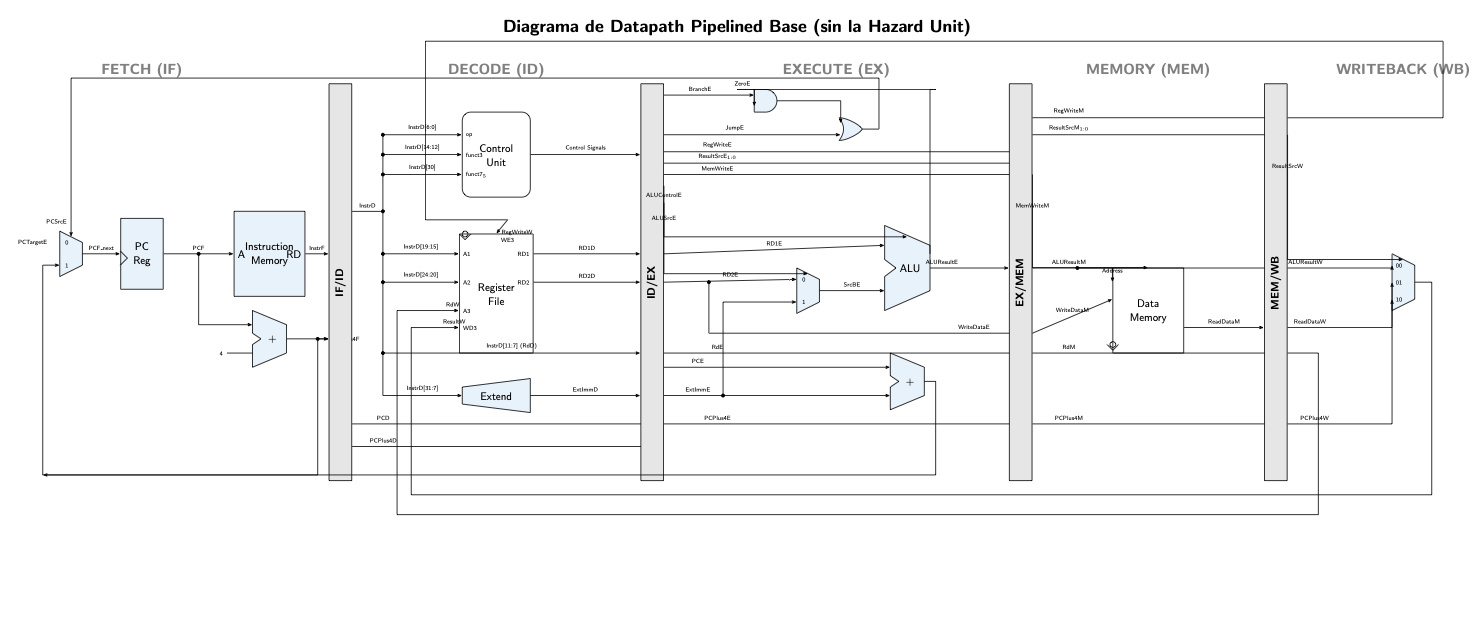
\includegraphics[width=\textwidth]{../Images/diagrama_base.png}
\caption{Diagrama del Datapath Pipelined básico del procesador (sin la Hazard Unit).}
\end{figure}

El datapath básico funciona dividiendo el camino crítico combinacional de la arquitectura de ciclo único en cinco etapas más cortas y balanceadas de forma paralela. En este diseño sin la Hazard Unit, el procesador opera correctamente bajo la suposición de que no existen dependencias de datos ni de control entre instrucciones consecutivas (o que estas se resuelven agregando instrucciones \texttt{nop} manuales en el ensamblador). Cada una de las etapas (\texttt{IF}, \texttt{ID}, \texttt{EX}, \texttt{MEM}, \texttt{WB}) ejecuta de forma concurrente una instrucción gracias a los registros de acoplamiento (\texttt{IF/ID}, \texttt{ID/EX}, \texttt{EX/MEM}, \texttt{MEM/WB}), los cuales retienen los operandos y las señales de control correspondientes. Esto permite completar la ejecución de una instrucción en cada ciclo de reloj (IPC ideal = 1) una vez que se ha llenado el pipeline.


\subsection{Los Registros Pipeline}

\subsubsection{¿Qué son y por qué son necesarios?}

Los registros pipeline \textbf{separan físicamente} una etapa de la siguiente. Sin ellos, las señales se mezclarían. Se ubican entre cada par de etapas.

\subsubsection{Tres Tipos de Flip-Flops}

\begin{figure}[H]
\centering
\begin{tikzpicture}[
  x=1cm, y=1cm,
  pin/.style={font=\tiny\sffamily, text=black, align=center},
  arrow/.style={-{Stealth}, thick, black},
]

% flopr (Centro en x=0)
\node[ffbox] (flopr) at (0, 0) {\textbf{flopr}\\[1mm]\scriptsize (Registro estándar)};
\clkpin{flopr}
\draw[arrow] (-2.5, 0.3) -- (flopr.west |- {0,0.3}) node[midway, above, pin] {d};
\draw[arrow] (flopr.east |- {0,0.3}) -- (2.5, 0.3) node[midway, above, pin] {q};
\node[pin, below=5mm of flopr] {Usado en: \textbf{EX/MEM, MEM/WB}\\[1mm](sin stall ni flush)};

% flopenr (Centro en x=5.3)
\node[ffbox] (flopenr) at (5.3, 0) {\textbf{flopenr}\\[1mm]\scriptsize (Con Enable)};
\clkpin{flopenr}
\draw[arrow] (2.9, 0.3) -- (flopenr.west |- {5.3,0.3}) node[midway, above, pin] {d};
\draw[arrow] (flopenr.east |- {5.3,0.3}) -- (7.7, 0.3) node[midway, above, pin] {q};
\draw[arrow] (5.3, 1.5) -- (5.3, 1.0) node[midway, right, pin] {en};
\node[pin, below=5mm of flopenr] {Usado en: \textbf{Registro PC}\\[1mm](con stall, sin flush)};

% flopenrc (Centro en x=10.6)
\node[ffbox] (flopenrc) at (10.6, 0) {\textbf{flopenrc}\\[1mm]\scriptsize (Enable y Clear)};
\clkpin{flopenrc}
\draw[arrow] (8.2, 0.3) -- (flopenrc.west |- {10.6,0.3}) node[midway, above, pin] {d};
\draw[arrow] (flopenrc.east |- {10.6,0.3}) -- (13.0, 0.3) node[midway, above, pin] {q};
\draw[arrow] (10.1, 1.5) -- (10.1, 1.0) node[midway, left, pin] {en};
\draw[arrow] (11.1, 1.5) -- (11.1, 1.0) node[midway, right, pin] {clear};
\node[pin, below=5mm of flopenrc] {Usado en: \textbf{IF/ID, ID/EX}\\[1mm](con stall y flush)};

\end{tikzpicture}
\caption{Los tres tipos de flip-flops usados. Observa el triángulo símbolo de la señal de reloj sincronizada por flanco.}
\end{figure}

\subsubsection{¿Por qué IF/ID usa flopenrc y MEM/WB usa flopr?}

Las etapas tempranas (Fetch, Decode, Execute) son \textbf{especulativas}: las instrucciones pueden ser descartadas (flush) si un salto cambia el flujo, o detenidas (stall) si hay una dependencia de datos sin resolver.

Las etapas tardías (Memory, Writeback) ejecutan instrucciones que ya \textbf{pasaron todos los filtros}: ya se resolvieron los saltos y los riesgos. Nunca hay razón para detenerlas ni vaciarlas, de ahí que solo requieran un \texttt{flopr} básico.

\begin{lstlisting}[style=pseudo, caption={Comportamiento de los registros pipeline}]
// flopenrc: Tiene clk, reset, enable y clear
always @(posedge clk):
  if (reset)      q = 0;
  else if (clear) q = 0; // FLUSH: inserta burbuja NOP
  else if (en)    q = d; // Avanza normalmente
  // else if (!en): q no cambia (CONGELADO - STALL)
\end{lstlisting}

\subsection{Módulo Top-Level: \texttt{riscv\_pipeline}}

El módulo \texttt{riscv\_pipeline} es el \textbf{ensamblaje principal} que conecta las 5 etapas con la Hazard Unit. Es puramente estructural, cableando todos los submóulos.

\begin{lstlisting}[style=verilogstyle, caption={Código Verilog del módulo top-level}]
module riscv_pipeline (
  input  logic clk, reset,
  output logic [31:0] PCF,
  output logic        MemWriteM
);
  // Cables para conectar las etapas
  // IF -> ID
  logic [31:0] InstrF, PCPlus4F;
  
  // ID -> EX
  logic [31:0] InstrD, PCD, PCPlus4D, RD1D, RD2D, ExtImmD;
  logic [4:0]  Rs1D, Rs2D, RdD;
  logic        RegWriteD, MemWriteD, JumpD, BranchD, ALUSrcD;
  logic [1:0]  ResultSrcD;
  logic [3:0]  ALUControlD;
  
  // EX -> MEM / Hazard
  logic        RegWriteE, MemWriteE, PCSrcE;
  logic [1:0]  ResultSrcE;
  logic [31:0] ALUResultE, WriteDataE, PCPlus4E, PCTargetE, InstrE;
  logic [4:0]  RdE, Rs1E, Rs2E;
  logic        ZeroE;
  
  // MEM -> WB / Hazard
  logic        RegWriteM_internal;
  logic [1:0]  ResultSrcM;
  logic [31:0] ALUResultM, ReadDataM, PCPlus4M, WriteDataM, InstrM;
  logic [4:0]  RdM;
  
  // WB -> Hazard / Decode
  logic        RegWriteW;
  logic [31:0] ResultW, InstrW;
  logic [4:0]  RdW;
  
  // Hazard Unit
  logic        StallF, StallD, FlushD, FlushE;
  logic [1:0]  ForwardAE, ForwardBE;

  // Instanciación de la etapa Fetch
  fetch fetchStage (
    .clk(clk), .reset(reset),
    .StallF(StallF), .PCSrcE(PCSrcE), .PCTargetE(PCTargetE),
    .InstrF(InstrF), .PCF(PCF), .PCPlus4F(PCPlus4F)
  );

  // Instanciación de la etapa Decode
  decode decodeStage (
    .clk(clk), .reset(reset),
    .StallD(StallD), .FlushD(FlushD),
    .InstrF(InstrF), .PCF(PCF), .PCPlus4F(PCPlus4F),
    .RegWriteW(RegWriteW), .RdW(RdW), .ResultW(ResultW),
    .InstrD(InstrD), .PCD(PCD), .PCPlus4D(PCPlus4D),
    .RD1D(RD1D), .RD2D(RD2D), .ExtImmD(ExtImmD),
    .Rs1D(Rs1D), .Rs2D(Rs2D), .RdD(RdD),
    .RegWriteD(RegWriteD), .ResultSrcD(ResultSrcD), .MemWriteD(MemWriteD),
    .JumpD(JumpD), .BranchD(BranchD), .ALUControlD(ALUControlD), .ALUSrcD(ALUSrcD)
  );

  // Instanciación de la etapa Execute
  execute executeStage (
    .clk(clk), .reset(reset),
    .FlushE(FlushE), .ForwardAE(ForwardAE), .ForwardBE(ForwardBE),
    .RegWriteD(RegWriteD), .ResultSrcD(ResultSrcD), .MemWriteD(MemWriteD),
    .JumpD(JumpD), .BranchD(BranchD), .ALUControlD(ALUControlD), .ALUSrcD(ALUSrcD),
    .RD1D(RD1D), .RD2D(RD2D), .PCD(PCD),
    .Rs1D(Rs1D), .Rs2D(Rs2D), .RdD(RdD),
    .ExtImmD(ExtImmD), .PCPlus4D(PCPlus4D), .InstrD(InstrD),
    .ALUResultM(ALUResultM), .ResultW(ResultW),
    .RegWriteE(RegWriteE), .ResultSrcE(ResultSrcE), .MemWriteE(MemWriteE),
    .ALUResultE(ALUResultE), .WriteDataE(WriteDataE), .RdE(RdE), .PCPlus4E(PCPlus4E), .InstrE(InstrE),
    .PCSrcE(PCSrcE), .PCTargetE(PCTargetE), .Rs1E(Rs1E), .Rs2E(Rs2E)
  );

  // Para conectar ZeroE que está interno a Execute si lo necesitamos en TB
  assign ZeroE = executeStage.ZeroE;

  // Instanciación de la etapa Memory
  memory_stage memStage (
    .clk(clk), .reset(reset),
    .RegWriteE(RegWriteE), .ResultSrcE(ResultSrcE), .MemWriteE(MemWriteE),
    .ALUResultE(ALUResultE), .WriteDataE(WriteDataE), .RdE(RdE), .PCPlus4E(PCPlus4E), .InstrE(InstrE),
    .RegWriteM(RegWriteM_internal), .ResultSrcM(ResultSrcM),
    .ALUResultM(ALUResultM), .ReadDataM(ReadDataM), .RdM(RdM), .PCPlus4M(PCPlus4M), .InstrM(InstrM)
  );
  
  // Extraemos variables internas de Memory para el Hazard Unit y el Testbench
  assign MemWriteM  = memStage.MemWriteM;
  assign WriteDataM = memStage.WriteDataM;

  // Instanciación de la etapa Writeback
  writeback wbStage (
    .clk(clk), .reset(reset),
    .RegWriteM(RegWriteM_internal), .ResultSrcM(ResultSrcM),
    .ALUResultM(ALUResultM), .ReadDataM(ReadDataM), .RdM(RdM), .PCPlus4M(PCPlus4M), .InstrM(InstrM),
    .RegWriteW(RegWriteW), .ResultW(ResultW), .RdW(RdW), .InstrW(InstrW)
  );

  // Instanciación de la Hazard Unit
  hunit hazardUnit (
    .Rs1E(Rs1E), .Rs2E(Rs2E), .RdM(RdM), .RdW(RdW),
    .RegWriteM(RegWriteM_internal), .RegWriteW(RegWriteW),
    .Rs1D(Rs1D), .Rs2D(Rs2D), .RdE(RdE),
    .ResultSrcE0(ResultSrcE[0]), .PCSrcE(PCSrcE),
    .ForwardAE(ForwardAE), .ForwardBE(ForwardBE),
    .StallF(StallF), .StallD(StallD),
    .FlushD(FlushD), .FlushE(FlushE)
  );

endmodule
\end{lstlisting}

\subsection{Etapa 1: Fetch (IF)}

\subsubsection{Componentes Activos}

\begin{figure}[H]
\centering
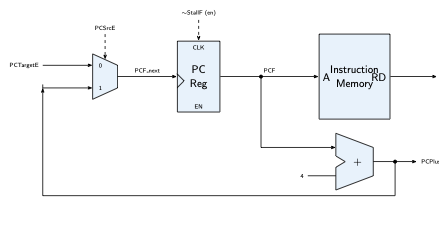
\includegraphics[width=0.85\textwidth]{../Images/fetch_stage.png}
\caption{Etapa Fetch aislada con sus componentes operativos.}
\end{figure}

\subsubsection{Código Verilog}

\begin{lstlisting}[style=verilogstyle, caption={Código Verilog de la etapa Fetch}]
module fetch (
  input  logic        clk, reset,
  input  logic        StallF,
  input  logic        PCSrcE,
  input  logic [31:0] PCTargetE,
  output logic [31:0] InstrF,
  output logic [31:0] PCF,
  output logic [31:0] PCPlus4F // Se mantiene este nombre de puerto para no romper el pipeline
);

  logic [31:0] PCF_next;
  logic [31:0] raw_imem_data;
  logic [31:0] actual_instr;
  logic [15:0] cinstr;
  logic [31:0] decompressed_instr;
  logic        is_compressed;
  logic [31:0] pc_increment;

  // Multiplexor del PC
  mux2 #(32) pcmux (
    .d0(PCPlus4F),
    .d1(PCTargetE),
    .s(PCSrcE),
    .y(PCF_next)
  );

  // Registro del PC
  flopenr #(32) pcReg (
    .clk(clk), .reset(reset), .en(~StallF),
    .d(PCF_next), .q(PCF)
  );

  // Memoria de Instrucciones
  imem imem_inst (
    .a(PCF),
    .rd(raw_imem_data)
  );

  // Lógica de Alineación (Extracción de la instrucción correcta)
  // Si PC[1] == 1, la instrucción empieza a la mitad de la palabra leída.
  assign actual_instr = PCF[1] ? {16'b0, raw_imem_data[31:16]} : raw_imem_data;

  // Extraemos solo los 16 bits menos significativos para el descompresor
  assign cinstr = actual_instr[15:0];

  // Instanciación del Descompresor
  decompressor decomp (
    .cinstr(cinstr),
    .outstr(decompressed_instr),
    .is_compressed(is_compressed)
  );

  // Mux Final: Seleccionamos la expandida (si era C) o pasamos la normal de 32-bits
  assign InstrF = is_compressed ? decompressed_instr : actual_instr;

  // Incremento Dinámico del PC
  assign pc_increment = is_compressed ? 32'd2 : 32'd4;

  adder pcadd (
    .a(PCF),
    .b(pc_increment),
    .y(PCPlus4F) // Ahora contiene PC + 2 o PC + 4 según corresponda
  );

endmodule
\end{lstlisting}

\subsection{Etapa 2: Decode (ID)}

\subsection{Componentes Activos}

\begin{figure}[H]
\centering
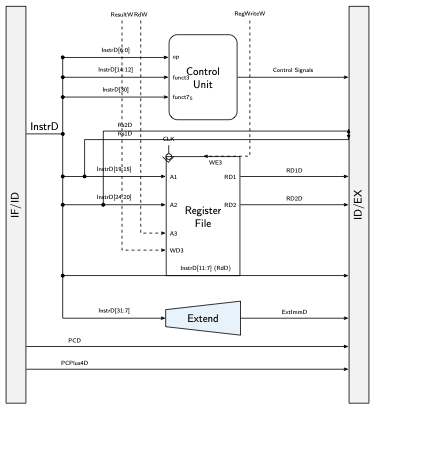
\includegraphics[width=0.85\textwidth]{../Images/decode_stage.png}
\caption{Etapa Decode aislada. Incluye el banco de registros y unidad de control.}
\end{figure}

\subsubsection{Unidad de Control}

La Unidad de Control recibe el \texttt{opcode}, \texttt{funct3} y \texttt{funct7} de la instrucción y genera todas las señales de control.

\begin{table}[H]
\centering
\small
\setlength{\tabcolsep}{4.5pt} % Evita desbordamiento de la tabla
\begin{tabular}{l|c|c|c|c|c|c|c|c}
\toprule
\textbf{Tipo} & \textbf{Opcode} & \textbf{RegW} & \textbf{ImmSrc} & \textbf{ALUSrc} & \textbf{MemW} & \textbf{ResSrc} & \textbf{Branch} & \textbf{ALUOp} \\
\midrule
lw      & 0000011 & 1 & 000 & 1 & 0 & 01 & 0 & 00 \\
sw      & 0100011 & 0 & 001 & 1 & 1 & -- & 0 & 00 \\
R-type  & 0110011 & 1 & xxx & 0 & 0 & 00 & 0 & 10 \\
I-type  & 0010011 & 1 & 000 & 1 & 0 & 00 & 0 & 10 \\
beq     & 1100011 & 0 & 010 & 0 & 0 & -- & 1 & 01 \\
jal     & 1101111 & 1 & 011 & 0 & 0 & 10 & 0 & xx \\
lui     & 0110111 & 1 & 100 & 1 & 0 & 00 & 0 & 11 \\
jalr    & 1100111 & 1 & 000 & 1 & 0 & 10 & 0 & 00 \\
\bottomrule
\end{tabular}
\caption{Tabla de verdad de la unidad de control principal.}
\end{table}

\textbf{Nota crítica sobre el ALUControl:} El \texttt{ALUControl} usa \textbf{4 bits}, no 3. El bit [3] diferencia ADD (0000) de SUB (1000). Si se truncara a 3 bits, la resta se interpretaría como suma y fallaría la operación \texttt{sub} o la lógica de comparación de \texttt{beq}.

\subsubsection{Código Verilog de Decode}

\begin{lstlisting}[style=verilogstyle, caption={Código Verilog de la etapa Decode}]
module decode (
  // Señales de reloj y reset
  input  logic        clk, reset,
  
  // Señales de control de la Hazard Unit (Riesgos)
  input  logic        StallD, FlushD,
  
  // Entradas desde la etapa Fetch (F)
  input  logic [31:0] InstrF, PCF, PCPlus4F,
  
  // Entradas desde la etapa Writeback (W) para el Register File
  input  logic        RegWriteW,
  input  logic [4:0]  RdW,
  input  logic [31:0] ResultW,
  
  // Salidas hacia la etapa Execute (E) - Datos
  output logic [31:0] InstrD, PCD, PCPlus4D,
  output logic [31:0] RD1D, RD2D,
  output logic [31:0] ExtImmD,
  output logic [4:0]  Rs1D, Rs2D, RdD,
  
  // Salidas hacia la etapa Execute (E) - Señales de Control
  output logic        RegWriteD,
  output logic [1:0]  ResultSrcD,
  output logic        MemWriteD,
  output logic        JumpD,
  output logic        BranchD,
  output logic [3:0]  ALUControlD,
  output logic        ALUSrcD
);

  // ==========================================================================
  // REGISTROS IF/ID (Pipeline Registers)
  // ==========================================================================
  
  // Registro para la Instrucción
  flopenrc #(32) ifIdInstr (
    .clk(clk), .reset(reset), .en(~StallD), .clear(FlushD),
    .d(InstrF), .q(InstrD)
  );

  // Registro para el Program Counter (PC)
  flopenrc #(32) ifIdPc (
    .clk(clk), .reset(reset), .en(~StallD), .clear(FlushD),
    .d(PCF), .q(PCD)
  );

  // Registro para PC + 4
  flopenrc #(32) ifIdPcPlus4 (
    .clk(clk), .reset(reset), .en(~StallD), .clear(FlushD),
    .d(PCPlus4F), .q(PCPlus4D)
  );

  // ==========================================================================
  // EXTRACCIÓN DE CAMPOS DE LA INSTRUCCIÓN
  // ==========================================================================
  
  assign Rs1D = InstrD[19:15]; // Source Register 1
  assign Rs2D = InstrD[24:20]; // Source Register 2
  assign RdD  = InstrD[11:7];  // Destination Register

  // ==========================================================================
  // COMPONENTES DE LA ETAPA DECODE
  // ==========================================================================

  // Register File: Banco de Registros
  // Lee de Rs1D y Rs2D de manera asíncrona (combinacional)
  // Escribe en RdW de manera síncrona en el flanco del reloj si RegWriteW = 1
  regfile rf (
    .clk(clk), .we3(RegWriteW),
    .a1(Rs1D), .a2(Rs2D), .a3(RdW),
    .wd3(ResultW), .rd1(RD1D), .rd2(RD2D)
  );

  // ImmSrcD es una señal de control local (solo se usa dentro de Decode)
  logic [2:0] ImmSrcD;

  // Control Unit: Decodifica la instrucción y genera las señales de control
  controller ctrl (
    .op(InstrD[6:0]),
    .funct3(InstrD[14:12]),
    .funct7(InstrD[31:25]),
    .RegWrite(RegWriteD),
    .ResultSrc(ResultSrcD),
    .MemWrite(MemWriteD),
    .Jump(JumpD),
    .Branch(BranchD),
    .ALUControl(ALUControlD),
    .ALUSrc(ALUSrcD),
    .ImmSrc(ImmSrcD)
  );

  // Extend Unit: Extiende el inmediato según el tipo de instrucción
  extend ext (
    .instr(InstrD[31:7]),
    .immsrc(ImmSrcD),
    .immext(ExtImmD)
  );

endmodule
\end{lstlisting}

% ============================================================================
% SECCION 6: ETAPA EXECUTE
% ============================================================================
\section{Etapa 3: Execute (EX)}

La etapa Execute es el núcleo de cálculo del procesador. Es aquí donde la ALU (Arithmetic Logic Unit) procesa los datos y toma decisiones críticas para el flujo del programa.

\textbf{Teoría Operativa:}
A diferencia de un procesador de ciclo único donde la decisión de saltar (Branch) se evalúa en Decode, en este pipeline se evalúa en Execute. La ALU realiza una resta (\texttt{sub}) entre los dos operandos y levanta la bandera \texttt{ZeroE} si son iguales. Esta bandera, al operarse mediante una compuerta AND con la señal \texttt{BranchE}, determina la señal \texttt{PCSrcE} (Branch Taken). 
Este retraso arquitectónico significa que el salto no se resuelve hasta el tercer ciclo, lo que introduce una penalización de 2 ciclos (burbujas) en caso de que el salto sea tomado, los cuales son gestionados puramente por la \textit{Hazard Unit}.

\subsection{Componentes Activos}

\begin{figure}[H]
\centering
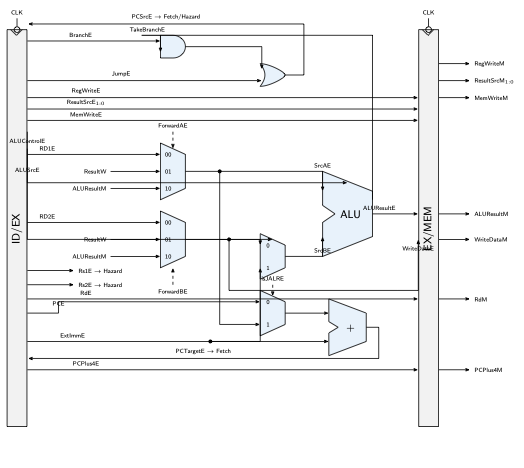
\includegraphics[width=0.85\textwidth]{../Images/execute_stage.png}
\caption{Etapa Execute. Muestra los multiplexores de Forwarding integrados antes de la ALU.}
\end{figure}

\subsection{Código Verilog de la etapa Execute}

\begin{lstlisting}[style=verilogstyle, caption={Código Verilog de la etapa Execute}]
module execute (
  // Señales de reloj y reset
  input  logic        clk, reset,
  
  // Señales de control de la Hazard Unit (Riesgos)
  input  logic        FlushE,
  input  logic [1:0]  ForwardAE, ForwardBE,
  
  // Entradas desde la etapa Decode (D) - Control
  input  logic        RegWriteD,
  input  logic [1:0]  ResultSrcD,
  input  logic        MemWriteD,
  input  logic        JumpD,
  input  logic        BranchD,
  input  logic [3:0]  ALUControlD, 
  input  logic        ALUSrcD,
  
  // Entradas desde la etapa Decode (D) - Datos
  input  logic [31:0] RD1D, RD2D,
  input  logic [31:0] PCD,
  input  logic [4:0]  Rs1D, Rs2D, RdD,
  input  logic [31:0] ExtImmD,
  input  logic [31:0] PCPlus4D,
  input  logic [31:0] InstrD,
  
  // Entradas desde Memory y Writeback (para Forwarding)
  input  logic [31:0] ALUResultM, ResultW,
  
  // Salidas hacia la etapa Memory (M) y Hazard Unit
  output logic        RegWriteE,
  output logic [1:0]  ResultSrcE,
  output logic        MemWriteE,
  output logic [31:0] ALUResultE, WriteDataE,
  output logic [4:0]  RdE,
  output logic [31:0] PCPlus4E,
  output logic [31:0] InstrE,
  
  // Salidas hacia Fetch y Hazard Unit
  output logic        PCSrcE,
  output logic [31:0] PCTargetE,
  output logic [4:0]  Rs1E, Rs2E
);

  // Cables internos de la etapa Execute (salidas del registro ID/EX)
  logic        JumpE, BranchE, ALUSrcE, ZeroE;
  logic [3:0]  ALUControlE;
  logic [31:0] RD1E, RD2E, PCE, ExtImmE;
  
  // Entradas a la ALU
  logic [31:0] SrcAE, SrcBE;

  // ==========================================================================
  // REGISTRO ID/EX (Pipeline Register)
  // ==========================================================================
  // Este registro separa la etapa de Decode de Execute. 
  // Ojo: En el diagrama no tiene Stall (siempre habilitado, en = 1'b1), pero sí tiene FlushE
  // para vaciarse cuando hay un salto fallido.
  // Tiene un total de 218 bits (Control + Datos).
  
  flopenrc #(218) idexReg (
    .clk(clk), .reset(reset), .en(1'b1), .clear(FlushE),
    .d({RegWriteD, ResultSrcD, MemWriteD, JumpD, BranchD, ALUControlD, ALUSrcD, 
        RD1D, RD2D, PCD, Rs1D, Rs2D, RdD, ExtImmD, PCPlus4D, InstrD}),
    .q({RegWriteE, ResultSrcE, MemWriteE, JumpE, BranchE, ALUControlE, ALUSrcE, 
        RD1E, RD2E, PCE, Rs1E, Rs2E, RdE, ExtImmE, PCPlus4E, InstrE})
  );

  // ==========================================================================
  // COMPONENTES DE LA ETAPA EXECUTE
  // ==========================================================================

  // Forwarding Mux para la entrada A de la ALU
  // Decide si usar RD1E, o un valor "adelantado" de Writeback o Memory
  mux3 #(32) forwardAmux (
    .d0(RD1E), 
    .d1(ResultW), 
    .d2(ALUResultM),
    .s(ForwardAE), 
    .y(SrcAE)
  );

  // Forwarding Mux para la entrada B de la ALU
  // Decide si usar RD2E, o un valor "adelantado" de Writeback o Memory
  // Nota: La salida de este mux es WriteDataE (el dato que se guardará en memoria)
  mux3 #(32) forwardBmux (
    .d0(RD2E), 
    .d1(ResultW), 
    .d2(ALUResultM),
    .s(ForwardBE), 
    .y(WriteDataE)
  );

  // Mux que selecciona el operando B de la ALU
  // (entre WriteDataE o el Inmediato Extendido)
  mux2 #(32) srcBmux (
    .d0(WriteDataE), 
    .d1(ExtImmE),
    .s(ALUSrcE), 
    .y(SrcBE)
  );

  // ALU (Unidad Aritmético Lógica)
  alu aluUnit (
    .a(SrcAE), 
    .b(SrcBE),
    .alucontrol(ALUControlE),
    .result(ALUResultE), 
    .zero(ZeroE)
  );
  logic        isJALRE;
  logic [31:0] pcTargetBaseE;
  logic [31:0] pcTargetAddOutE;
  logic        TakeBranchE;

  // Detección local de JALR en Execute
  assign isJALRE = (InstrE[6:0] == 7'b1100111);
  assign pcTargetBaseE = isJALRE ? SrcAE : PCE;

  // Sumador para la dirección de salto (PC o registro base + Inmediato Extendido)
  adder pcTargetAdd (
    .a(pcTargetBaseE), 
    .b(ExtImmE), 
    .y(pcTargetAddOutE)
  );

  // El bit menos significativo de la dirección calculada por jalr se limpia
  assign PCTargetE = {pcTargetAddOutE[31:1], 1'b0};

  // Lógica para decidir si se toma el salto para distintas condiciones
  always_comb begin
    case (InstrE[14:12])
      3'b000:  TakeBranchE = ZeroE;                     // beq
      3'b001:  TakeBranchE = ~ZeroE;                    // bne
      3'b100:  TakeBranchE = $signed(SrcAE) < $signed(SrcBE); // blt
      3'b101:  TakeBranchE = $signed(SrcAE) >= $signed(SrcBE); // bge
      3'b110:  TakeBranchE = SrcAE < SrcBE;             // bltu
      3'b111:  TakeBranchE = SrcAE >= SrcBE;            // bgeu
      default: TakeBranchE = 1'b0;
    endcase
  end

  // PCSrcE = 1 si ocurre un Branch válido y se cumple la condición, o si es un Jump
  assign PCSrcE = (BranchE & TakeBranchE) | JumpE;

endmodule
\end{lstlisting}

% ============================================================================
% SECCION 7: ETAPA MEMORY Y WRITEBACK
% ============================================================================
\section{Etapas Memory (MEM) y Writeback (WB)}

Estas dos etapas finales son responsables de confirmar los resultados arquitectónicos, ya sea interactuando con la jerarquía de memoria o actualizando el banco de registros.

\textbf{Teoría de Memoria y Sincronismo:}
La Memoria de Datos representa típicamente la caché L1 de datos en un procesador real. En nuestra implementación, la memoria es \textbf{síncrona para escritura y asíncrona para lectura}. 
\begin{itemize}
    \item \textbf{Escritura:} Solo ocurre en el flanco de subida del reloj cuando \texttt{MemWriteM} está en alto. Esto evita que señales inestables modifiquen el estado de la memoria.
    \item \textbf{Lectura:} Las memorias reales modernas suelen ser síncronas para lectura también (añadiendo latencia), pero nuestra implementación combinacional simplificada asume que el dato se lee instantáneamente si la dirección (\texttt{ALUResultM}) es válida.
\end{itemize}

\subsection{Componentes Activos}

\begin{figure}[H]
\centering
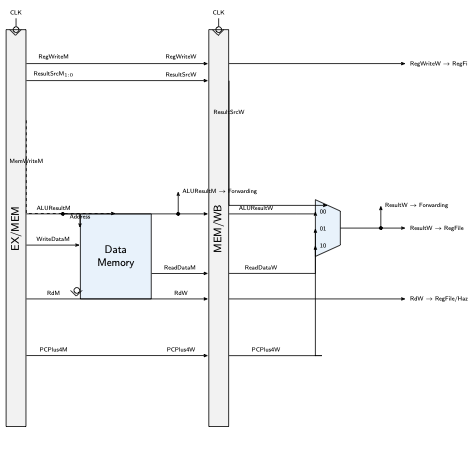
\includegraphics[width=0.85\textwidth]{../Images/memory_writeback_stage.png}
\caption{Etapas Memory y Writeback. La memoria de datos tiene escritura síncrona.}
\end{figure}

\subsection{Código Verilog de las etapas Memory y Writeback}

\begin{lstlisting}[style=verilogstyle, caption={Código Verilog de la etapa Memory}]
module memory_stage (
  // Señales de reloj y reset
  input  logic        clk, reset,
  
  // Entradas desde la etapa Execute (E)
  input  logic        RegWriteE,
  input  logic [1:0]  ResultSrcE,
  input  logic        MemWriteE,
  input  logic [31:0] ALUResultE, WriteDataE,
  input  logic [4:0]  RdE,
  input  logic [31:0] PCPlus4E,
  input  logic [31:0] InstrE,
  
  // Salidas hacia la etapa Writeback (W) y Forwarding
  output logic        RegWriteM,
  output logic [1:0]  ResultSrcM,
  output logic [31:0] ALUResultM,
  output logic [31:0] ReadDataM,
  output logic [4:0]  RdM,
  output logic [31:0] PCPlus4M,
  output logic [31:0] InstrM
);

  // Cables internos
  logic        MemWriteM;
  logic [31:0] WriteDataM;                

  // ==========================================================================
  // REGISTRO EX/MEM (Pipeline Register)
  // ==========================================================================
  // Separa la etapa de Execute de Memory. 
  // En el diagrama base de RISC-V, este registro NO tiene Stall ni Flush.
  // Pasan 137 bits en total: 5 bits de Control + 132 bits de Datos.
  
  flopr #(137) exmemReg (
    .clk(clk), .reset(reset),
    .d({RegWriteE, ResultSrcE, MemWriteE, ALUResultE, WriteDataE, RdE, PCPlus4E, InstrE}),
    .q({RegWriteM, ResultSrcM, MemWriteM, ALUResultM, WriteDataM, RdM, PCPlus4M, InstrM})
  );

  // ==========================================================================
  // COMPONENTES DE LA ETAPA MEMORY
  // ==========================================================================

  // Data Memory: Memoria de Datos
  // Usa ALUResultM como dirección de memoria y WriteDataM como el dato a guardar.
  // Solo escribe si MemWriteM está activo.
  dmem dataMemory (
    .clk(clk), 
    .we(MemWriteM),
    .a(ALUResultM), 
    .wd(WriteDataM),
    .rd(ReadDataM)
  );

endmodule
\end{lstlisting}

\begin{lstlisting}[style=verilogstyle, caption={Código Verilog de la etapa Writeback}]
module writeback (
  // Señales de reloj y reset
  input  logic        clk, reset,
  
  // Entradas desde la etapa Memory (M)
  input  logic        RegWriteM,
  input  logic [1:0]  ResultSrcM,
  input  logic [31:0] ALUResultM, ReadDataM,
  input  logic [4:0]  RdM,
  input  logic [31:0] PCPlus4M,
  input  logic [31:0] InstrM,
  
  // Salidas hacia la etapa Decode (D) y Forwarding
  output logic        RegWriteW,
  output logic [31:0] ResultW,
  output logic [4:0]  RdW,
  output logic [31:0] InstrW
);

  // Cables internos (salidas del registro MEM/WB)
  logic [1:0]  ResultSrcW;
  logic [31:0] ALUResultW, ReadDataW, PCPlus4W;

  // ==========================================================================
  // REGISTRO MEM/WB (Pipeline Register)
  // ==========================================================================
  // Separa la etapa de Memory de Writeback. 
  // No tiene Stall ni Flush en el diseño básico.
  // Pasan 136 bits en total: 4 bits de Control + 132 bits de Datos.
  
  flopr #(136) memwbReg (
    .clk(clk), .reset(reset),
    .d({RegWriteM, ResultSrcM, ALUResultM, ReadDataM, RdM, PCPlus4M, InstrM}),
    .q({RegWriteW, ResultSrcW, ALUResultW, ReadDataW, RdW, PCPlus4W, InstrW})
  );

  // ==========================================================================
  // COMPONENTES DE LA ETAPA WRITEBACK
  // ==========================================================================

  // Multiplexor de Resultado
  // Selecciona qué dato se guardará en el Register File (o se reenviará por forwarding)
  // 00 -> Resultado de la ALU
  // 01 -> Dato leído de la Memoria
  // 10 -> PC + 4 (Usado típicamente para llamadas a funciones: JAL/JALR)
  mux3 #(32) resultMux (
    .d0(ALUResultW), 
    .d1(ReadDataW), 
    .d2(PCPlus4W),
    .s(ResultSrcW), 
    .y(ResultW)
  );

endmodule
\end{lstlisting}

% ============================================================================
% SECCION 3: PROGRAMA ISA SIN DEPENDENCIAS (1.0 pts)
% ============================================================================
\section{Programa ISA sin Dependencias (1.0 pts)}

Este programa prueba que las instrucciones básicas del procesador (\texttt{addi}, \texttt{add}, \texttt{sw}, \texttt{lw}) funcionan correctamente cuando \textbf{no existen dependencias de datos entre instrucciones consecutivas}. Para lograrlo, se insertan instrucciones \texttt{nop} (no-operation) entre cada instrucción real, dando tiempo suficiente para que los datos se escriban en los registros antes de ser leídos por la siguiente instrucción.

\subsection{Código Ensamblador}
\begin{lstlisting}[style=pseudo, caption={Programa 1: ISA sin dependencias (test\_isa\_sin\_dependencias.mem)}]
00: addi x2, x0, 5       // x2 = 5
04: nop                   // Separador
08: nop
0C: nop
10: add  x3, x2, x2      // x3 = 10
14: nop
18: nop
1C: nop
20: sw   x3, 100(x0)     // MEM[100] = 10
24: nop
28: nop
2C: nop
30: lw   x4, 100(x0)     // x4 = MEM[100] = 10
34: nop
38: nop
3C: nop
40: add  x5, x4, x3      // x5 = 10 + 10 = 20
44: sw   x5, 200(x0)     // MEM[200] = 20
\end{lstlisting}

\subsection{Waveform del Programa 1}

\begin{figure}[H]
\centering
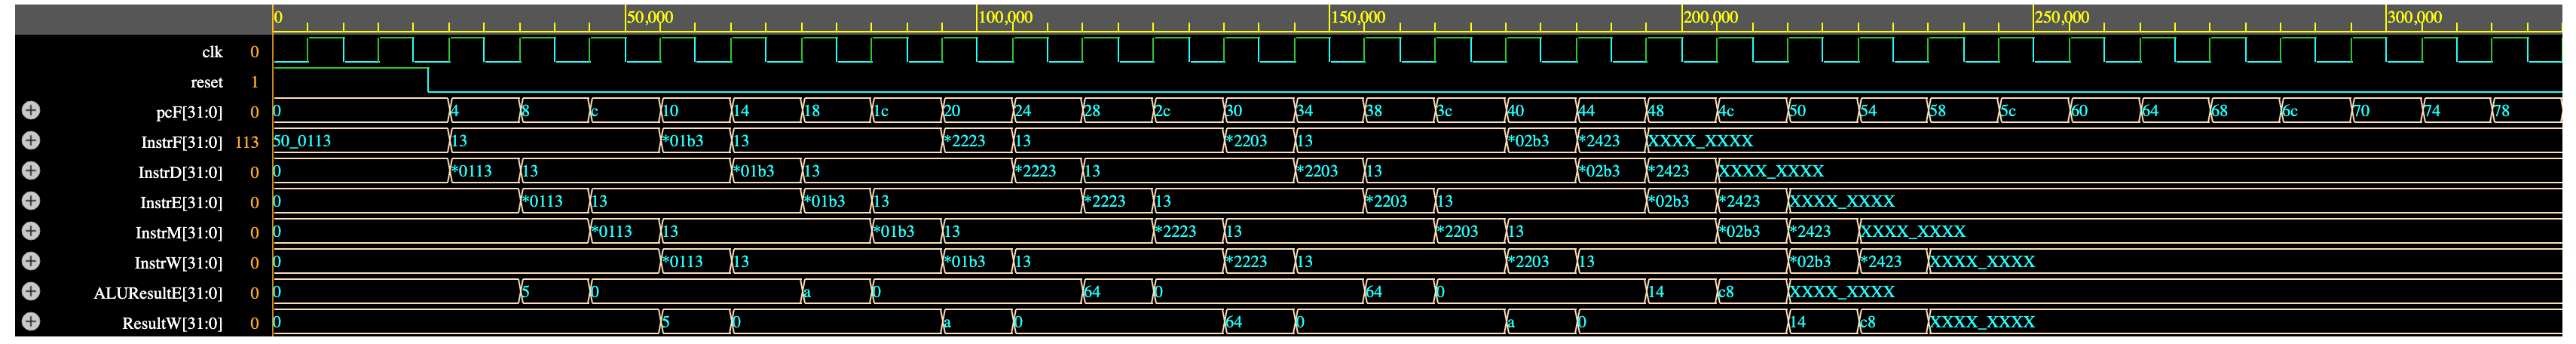
\includegraphics[width=0.88\textwidth]{../Images/waves_isa.png}
\caption{Waveform del Programa 1 (ISA sin dependencias). Las señales ForwardAE, ForwardBE, StallD y FlushE permanecen en 0 durante toda la ejecución.}
\end{figure}

\subsection{Mostrar con Resultados Intermedios que el Programa Funciona Correctamente}
Al observar el waveform, se verifica que:
\begin{itemize}
  \item La señal \texttt{ALUResultE} muestra el valor \texttt{0x05} cuando \texttt{addi x2, x0, 5} pasa por Execute, y \texttt{0x0A} cuando \texttt{add x3, x2, x2} lo hace.
  \item La señal \texttt{ResultW} confirma que el valor \texttt{0x14} (20 en decimal) llega correctamente al final del pipeline como resultado de \texttt{add x5, x4, x3}.
  \item Las señales de la Hazard Unit (\texttt{ForwardAE}, \texttt{ForwardBE}, \texttt{StallD}, \texttt{FlushE}) permanecen en 0, demostrando que no se activó ningún mecanismo de protección. El programa fluye sin interrupciones.
\end{itemize}

% ============================================================================
% SECCION 4: TEORIA DE HAZARD UNIT Y EVIDENCIA DE FALLOS (0.5 pts)
% ============================================================================
\section{Teoría de Hazard Unit y Evidencia de Fallos (0.5 pts)}

\subsection{Teoría de Control de Riesgos en Procesadores Segmentados}

Al segmentar la ejecución de instrucciones, se solapan las etapas del datapath, rompiendo la ejecución estrictamente secuencial. Esto puede dar lugar a \textbf{riesgos} (hazards) que comprometen la integridad de los resultados si no se resuelven mediante hardware especializado:

\begin{itemize}
    \item \textbf{Riesgos Estructurales (Structural Hazards):} Ocurren cuando dos instrucciones en etapas diferentes intentan acceder al mismo recurso físico al mismo tiempo. En este procesador se resuelven mediante una \textit{Arquitectura Harvard}, que separa físicamente la memoria de instrucciones de la memoria de datos.
    \item \textbf{Riesgos de Datos (Data Hazards):} Surgen cuando una instrucción depende del resultado de una instrucción previa que aún no ha completado su escritura en el Register File. El caso más frecuente es la dependencia RAW (Read After Write).
    \item \textbf{Riesgos de Control (Control Hazards):} Producidos por instrucciones de salto condicional (\texttt{beq}) o absoluto (\texttt{jal}). Al leer la instrucción en Fetch, el procesador continúa cargando secuencialmente. Si el salto se resuelve como tomado en Execute, las instrucciones cargadas especulativamente en Fetch y Decode son incorrectas y deben descartarse.
\end{itemize}

\subsection{Evidencia: Sin Hazard Unit los Programas Fallan}

Para demostrar de forma empírica la necesidad crítica de la Hazard Unit, se procedió a desactivar el control de riesgos utilizando el módulo alternativo \texttt{hunit\_disabled.v}. Este fuerza a cero los reenvíos y stalls. A continuación, se muestra el comportamiento de los programas de prueba bajo esta condición errónea:

\subsubsection{Programa 2 SIN Hazard Unit (Forwarding)}

Para este caso, se ejecuta el Programa 2, el cual intenta realizar operaciones aritméticas sobre registros cuyos resultados aún no han sido escritos en el banco de registros:

\begin{lstlisting}[style=pseudo, caption={Programa 2: test\_forwarding.mem (para deshabilitado)}]
00: addi x2, x0, 5       // x2 = 5
04: addi x3, x0, 12      // x3 = 12
08: add  x4, x2, x3      // x4 = 5 + 12 = 17 (Riesgo RAW)
0C: sw   x4, 200(x0)     // MEM[200] = 17
\end{lstlisting}

\begin{figure}[H]
\centering
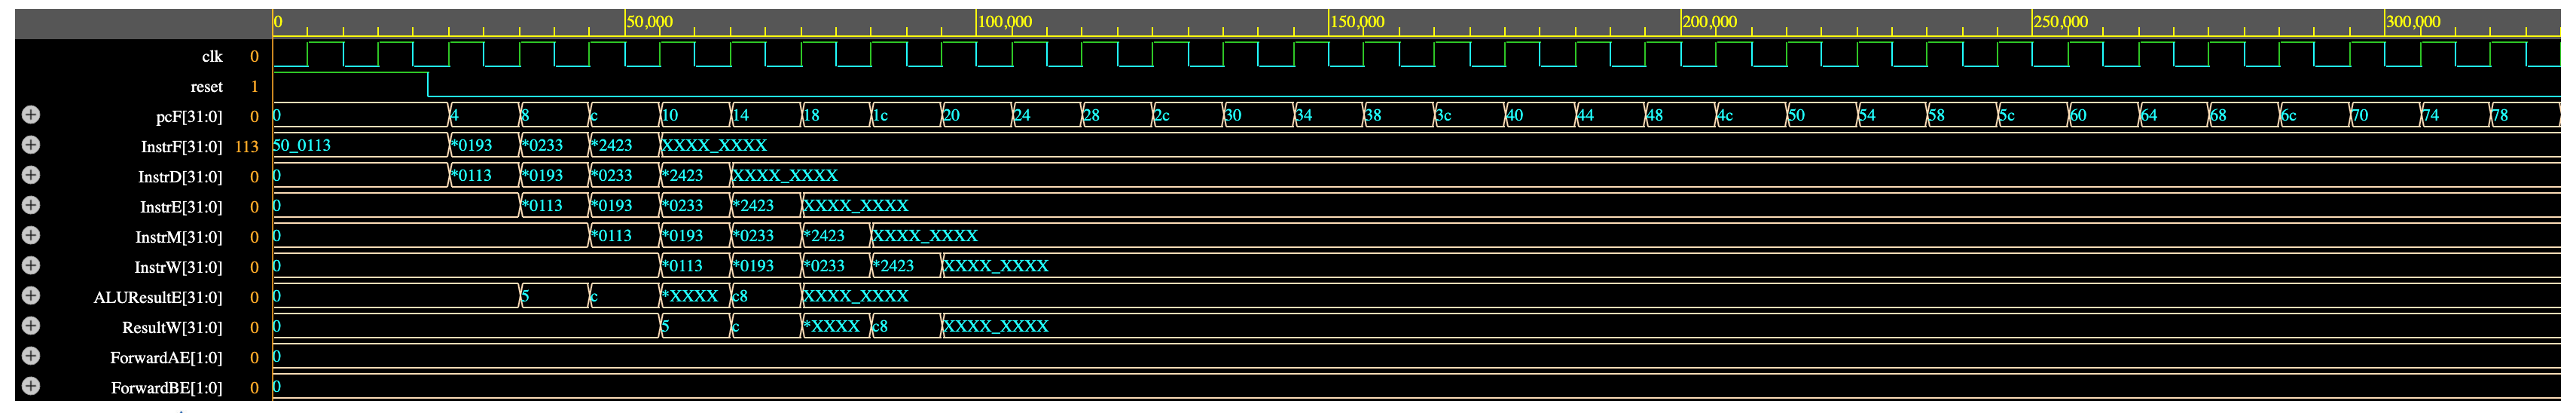
\includegraphics[width=0.80\textwidth]{../Images/waves_forwarding_NO_HAZARD.png}
\caption{Programa 2 SIN Hazard Unit. La ALU opera con datos vacíos (0x00) porque los registros x2 y x3 aún no se han escrito cuando el \texttt{add} los necesita.}
\end{figure}

\textbf{Análisis de Falla de Dependencia RAW en el Ciclo de Reloj:}
\begin{enumerate}
  \item La instrucción \texttt{addi x2, x0, 5} calcula el valor \texttt{5} en el ciclo 3 (etapa Execute) y avanza.
  \item La instrucción \texttt{addi x3, x0, 12} calcula el valor \texttt{12} en el ciclo 4 (etapa Execute).
  \item En el ciclo 4, la instrucción \texttt{add x4, x2, x3} se encuentra en la etapa \textbf{Decode} y realiza la lectura física del banco de registros. Dado que el banco de registros solo actualiza sus salidas al final de la etapa de Writeback (lo cual ocurre en el ciclo 5 para \texttt{x2} y ciclo 6 para \texttt{x3}), los valores leídos para ambos registros son \texttt{0x00000000} (los valores antiguos o nulos).
  \item En el ciclo 5, la instrucción \texttt{add x4} avanza a la etapa \textbf{Execute}. Sin la Hazard Unit, las señales de control de reenvío se desactivan (\texttt{ForwardAE = 00}, \texttt{ForwardBE = 00}). La ALU efectúa la operación básica sin corregir los operandos:
  \[ \text{Resultado} = 0 + 0 = 0 \]
  \item En lugar de almacenar \texttt{17} (\texttt{0x11}) en el registro \texttt{x4}, se escribe el valor erróneo \texttt{0} en el banco de registros al completar Writeback en el ciclo 7.
\end{enumerate}
\textbf{Error:} La dependencia de datos tipo \textit{Read After Write} (RAW) es completamente ignorada por el datapath, resultando en la corrupción silenciosa del resultado aritmético.

\subsubsection{Programa 3 SIN Hazard Unit (Stalling)}

En esta prueba se ejecuta el Programa 3, el cual presenta una dependencia de tipo Load-Use, requiriendo el uso inmediato de un dato cargado de memoria:

\begin{lstlisting}[style=pseudo, caption={Programa 3: test\_stalling.mem (para deshabilitado)}]
00: addi x2, x0, 5       // x2 = 5
04: sw   x2, 100(x0)     // MEM[100] = 5
08: lw   x3, 100(x0)     // x3 = MEM[100] = 5
0C: add  x4, x3, x2      // Load-Use Hazard (add usa x3 inmediatamente)
10: sw   x4, 200(x0)     // MEM[200] = 10
\end{lstlisting}

\begin{figure}[H]
\centering
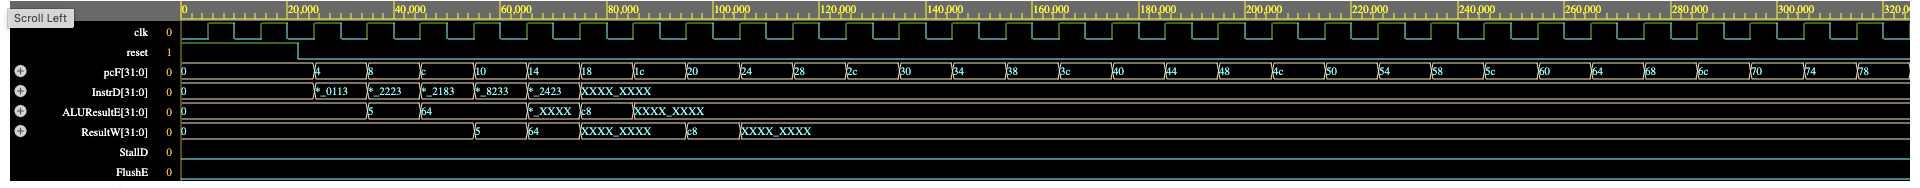
\includegraphics[width=0.82\textwidth]{../Images/waves_stalling_NO_HAZARD.png}
\caption{Programa 3 SIN Hazard Unit. El \texttt{add x4, x3, x2} usa un valor de x3 que aún no ha salido de la memoria.}
\end{figure}

\textbf{Análisis de Falla de Dependencia Load-Use en el Ciclo de Reloj:}
\begin{enumerate}
  \item La instrucción \texttt{lw x3, 100(x0)} calcula la dirección física de la memoria (\texttt{100}) en el ciclo 5 (etapa Execute) y realiza el acceso de lectura a la RAM en el ciclo 6 (etapa Memory).
  \item En el ciclo 6, la instrucción \texttt{add x4, x3, x2} está en la etapa \textbf{Execute} y requiere como operando el dato cargado de la memoria en \texttt{x3}.
  \item Puesto que la memoria de datos devuelve el valor leído al final de la etapa de Memory (ciclo 6), físicamente es imposible proveer dicho dato a la ALU en el ciclo 6 sin detener previamente el flujo del procesador por al menos un ciclo.
  \item Sin la Hazard Unit, no se generan las señales de detención (\texttt{StallF = 0}, \texttt{StallD = 0}). El procesador no inserta ninguna burbuja de espera (NOP). La instrucción \texttt{add x4} continúa en Execute leyendo el contenido obsoleto del banco de registros (\texttt{x3 = 0}).
  \item La ALU realiza la suma de forma incorrecta:
  \[ \text{Resultado} = x3_{\text{antiguo}} + x2 = 0 + 5 = 5 \]
  \item En el ciclo 7, el dato real leído de la memoria por \texttt{lw} (\texttt{5}) llega a la etapa de Writeback, pero el pipeline ya ha procesado la operación \texttt{add} con el valor corrupto, escribiendo un resultado erróneo en el banco de registros.
\end{enumerate}
\textbf{Error:} El pipeline no congela las etapas de Fetch y Decode, provocando que la instrucción consumidora intente operar con el bus de memoria antes de que la lectura física haya culminado.

\subsubsection{Programa 4 SIN Hazard Unit (Flushing)}

Para evaluar los riesgos de control se ejecuta el Programa 4, el cual realiza un salto condicional tomado que debería descartar las instrucciones siguientes cargadas de forma especulativa:

\begin{lstlisting}[style=pseudo, caption={Programa 4: test\_flushing.mem (para deshabilitado)}]
00: addi x2, x0, 5       // x2 = 5
04: beq  x2, x2, 12      // Salta a línea 10 hex (siempre verdadero)
08: addi x3, x0, 1       // FLUSHED (no debe ejecutarse)
0C: addi x3, x0, 99      // FLUSHED (no debe ejecutarse)
10: add  x4, x0, x2      // x4 = 5 (destino del salto)
14: sw   x4, 200(x0)     // MEM[200] = 5
\end{lstlisting}

\begin{figure}[H]
\centering
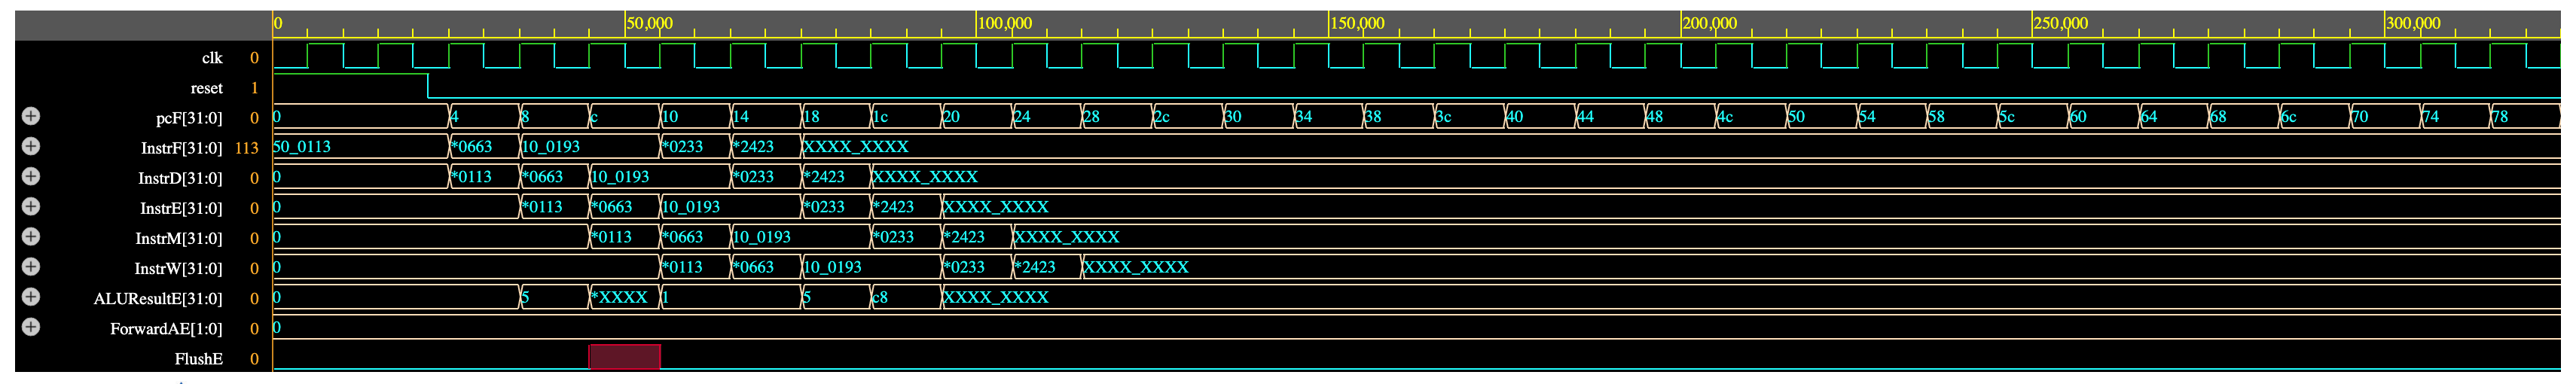
\includegraphics[width=0.84\textwidth]{../Images/waves_flushing_NO_HAZARD.png}
\caption{Programa 4 SIN Hazard Unit. Sin forwarding, las instrucciones previas al salto calculan incorrectamente, afectando la comparación del \texttt{beq}.}
\end{figure}

\textbf{Análisis de Pérdida de Control en Saltos en el Ciclo de Reloj:}
\begin{enumerate}
  \item En el ciclo 4, la instrucción \texttt{beq x2, x2, 12} está en la etapa \textbf{Execute}. La ALU detecta la igualdad de los registros y activa la señal de redirección del PC (\texttt{PCSrcE = 1}).
  \item Sin embargo, debido a la precarga secuencial inherente de la segmentación, durante los ciclos de decodificación del salto, el procesador ya ha ingresado las instrucciones de las direcciones consecutivas \texttt{0x08} (etapa Decode) y \texttt{0x0C} (etapa Fetch).
  \item Al estar la Hazard Unit desactivada, las señales de vaciado de etapa permanecen inactivas (\texttt{FlushD = 0}, \texttt{FlushE = 0}). Los registros de acoplamiento \texttt{IF/ID} y \texttt{ID/EX} no limpian su contenido.
  \item En consecuencia, durante los ciclos 5 y 6, las instrucciones de la ruta especulativa errónea (\texttt{addi x3, x0, 1} y \texttt{addi x3, x0, 99}) continúan avanzando a través de Execute, Memory y Writeback, modificando el estado del banco de registros al escribir \texttt{99} en el registro \texttt{x3}.
\end{enumerate}
\textbf{Error:} Se ejecutan instrucciones especulativas ubicadas en el camino secuencial posterior a un salto tomado. Esto corrompe los registros y la memoria de datos con valores correspondientes a un camino de ejecución prohibido.


% ============================================================================
% SECCION 5: IMPLEMENTACION DEL HAZARD UNIT (1.0 pts)
% ============================================================================
\section{Implementación del Hazard Unit (1.0 pts)}

\subsection{Descripción de Cambios en el Código}

Para gestionar los riesgos de datos y de control de forma transparente para el programador (sin tener que inyectar NOPs manuales en el ensamblador), se implementó el módulo \texttt{hunit} (\texttt{Hazard Unit}) en el archivo \texttt{Hazard Unit/hunit.v}. Los principales cambios e implementaciones en el código incluyen:

\begin{enumerate}
  \item \textbf{Diseño de la Unidad de Control de Riesgos:} Se diseñó un módulo puramente combinacional que monitorea las señales del datapath de forma continua y genera señales de bypass y de control en las etapas críticas.
  \item \textbf{Estrategia de Pruebas de Fallo sin Dañar el Diseño:} Con el fin de demostrar la necesidad de la Hazard Unit sin modificar el procesador, se creó la unidad \texttt{hunit\_disabled.v}. Este archivo tiene la misma firma (entradas y salidas) que la unidad real, pero inyecta un estado inactivo permanente (forzando reenvíos y stalls a 0), excepto por la redirección de saltos básicos para evitar que el PC entre en un ciclo infinito. La alternancia entre la simulación correcta y la errónea se realiza modificando una sola palabra en la instanciación del top-level (\texttt{riscv\_pipeline.v}).
\end{enumerate}

A continuación, se presentan los tres mecanismos principales de la unidad junto con sus diagramas y ecuaciones lógicas:

\begin{figure}[H]
\centering
\begin{tikzpicture}[
  x=1cm, y=1cm,
  hubox/.style={draw, thick, fill=pastelblue, minimum width=8cm, minimum height=2.5cm, font=\small\sffamily\bfseries, align=center},
  signalin/.style={-{Stealth}, thick},
  signalout/.style={-{Stealth}, thick, black},
  lblin/.style={font=\tiny\sffamily, above},
  lblout/.style={font=\tiny\sffamily, right},
]

\node[hubox] (hu) at (0, 0) {Hazard Unit};

% Entradas (arriba y laterales)
\draw[signalin] (-3, 2.5) -- (-3, 1.25) node[lblin, pos=0] {Rs1E, Rs2E};
\draw[signalin] (-1, 2.5) -- (-1, 1.25) node[lblin, pos=0] {RdM, RdW};
\draw[signalin] (1, 2.5) -- (1, 1.25) node[lblin, pos=0] {RegWriteM/W};
\draw[signalin] (3, 2.5) -- (3, 1.25) node[lblin, pos=0] {Rs1D, Rs2D, RdE};

\draw[signalin] (-5.5, 0.5) -- (-4, 0.5) node[lblin, pos=0, left] {ResultSrcE[0]};
\draw[signalin] (-5.5, -0.5) -- (-4, -0.5) node[lblin, pos=0, left] {PCSrcE};

% Salidas (abajo)
\draw[signalout] (-3, -1.25) -- (-3, -2.5) node[lblout, pos=1] {ForwardAE[1:0]};
\draw[signalout] (-1.5, -1.25) -- (-1.5, -2.5) node[lblout, pos=1] {ForwardBE[1:0]};
\draw[signalout] (0, -1.25) -- (0, -2.5) node[lblout, pos=1] {StallF};
\draw[signalout] (1, -1.25) -- (1, -2.5) node[lblout, pos=1] {StallD};
\draw[signalout] (2, -1.25) -- (2, -2.5) node[lblout, pos=1] {FlushD};
\draw[signalout] (3, -1.25) -- (3, -2.5) node[lblout, pos=1] {FlushE};

\end{tikzpicture}
\caption{Diagrama de la Hazard Unit y sus múltiples conexiones.}
\end{figure}

\subsection{Mecanismo 1: Forwarding (Reenvío de Datos)}
El forwarding (o bypassing) es la solución de hardware más elegante para resolver los \textbf{Data Hazards} tipo RAW. Teóricamente, un resultado se calcula en la etapa Execute (ALU), pero arquitectónicamente no se escribe en el Register File hasta la etapa de Writeback (2 ciclos después). Si una instrucción posterior necesita este resultado inmediatamente, no puede leer el registro porque contiene un valor "viejo".

La Hazard Unit detecta que el registro destino de una instrucción en MEM o WB ($RdM$ o $RdW$) coincide con los registros fuente de la instrucción actualmente en Execute ($Rs1E$ o $Rs2E$). Al detectarlo, \textbf{cortocircuita} los multiplexores para inyectar el dato recién salido de la ALU (o de la Memoria) directamente en la entrada de la ALU de la instrucción actual, saltándose la espera por el Writeback.

\begin{lstlisting}[style=pseudo, caption={Lógica de Forwarding}]
// Forwarding para operando A (SrcAE)
if ((Rs1E == RdM) && RegWriteM && (Rs1E != 0)):
    ForwardAE = 2'b10;    // Tomar resultado de Memory
else if ((Rs1E == RdW) && RegWriteW && (Rs1E != 0)):
    ForwardAE = 2'b01;    // Tomar resultado de Writeback
else:
    ForwardAE = 2'b00;    // Sin forwarding (usar registro)

// Forwarding para operando B (misma lógica con Rs2E)
\end{lstlisting}

\subsection{Mecanismo 2: Stall (Load-Use Hazard)}
El forwarding no puede resolver el Load-Use hazard (cuando un \texttt{lw} es seguido inmediatamente por una instrucción que lo usa). En ese caso, la Hazard Unit congela (stall) el PC y el IF/ID, e inserta una burbuja (flush) en el ID/EX.

\begin{lstlisting}[style=pseudo, caption={Lógica de detección de Load-Use Hazard}]
// ResultSrcE[0] == 1 indica que la instrucción es un lw
lwStall = ResultSrcE[0] && ((Rs1D == RdE) || (Rs2D == RdE));

StallF = lwStall;    // Congelar PC (no avanza)
StallD = lwStall;    // Congelar IF/ID (mantener instrucción)
FlushE = lwStall;    // Vaciar ID/EX (insertar burbuja NOP)
\end{lstlisting}

\subsection{Mecanismo 3: Flush (Control Hazard por Saltos)}
Cuando se toma un salto (\texttt{PCSrcE=1}), las instrucciones que entraron especulativamente al Fetch y Decode deben descartarse, vaciando sus registros.

\begin{lstlisting}[style=pseudo, caption={Lógica de flush por salto tomado}]
FlushD = PCSrcE;              // Vaciar IF/ID (descarta especulativa)
FlushE = lwStall || PCSrcE;   // Vaciar ID/EX
\end{lstlisting}

\subsection{Especificación de Señales de Control de Riesgos}
\begin{table}[H]
\centering
\small
\setlength{\tabcolsep}{5pt} % Evita desbordamiento de la tabla
\begin{tabular}{l|l|l|c}
\toprule
\textbf{Problema} & \textbf{Solución} & \textbf{Señales} & \textbf{Penalización} \\
\midrule
Data Hazard (R-type) & Forwarding & ForwardAE, ForwardBE & 0 ciclos \\
Load-Use Hazard & Stall + Forwarding & StallF, StallD, FlushE & 1 ciclo \\
Control Hazard & Flush & FlushD, FlushE & 2 ciclos \\
\bottomrule
\end{tabular}
\end{table}

\subsection{Diagrama de Datapath Final (con Hazard Unit)}

El datapath completo con todas las compuertas de control de riesgos, los multiplexores de forwarding para SrcAE y SrcBE, y las señales de stall y clear de los registros del pipeline se muestra a continuación:

\begin{figure}[H]
\centering
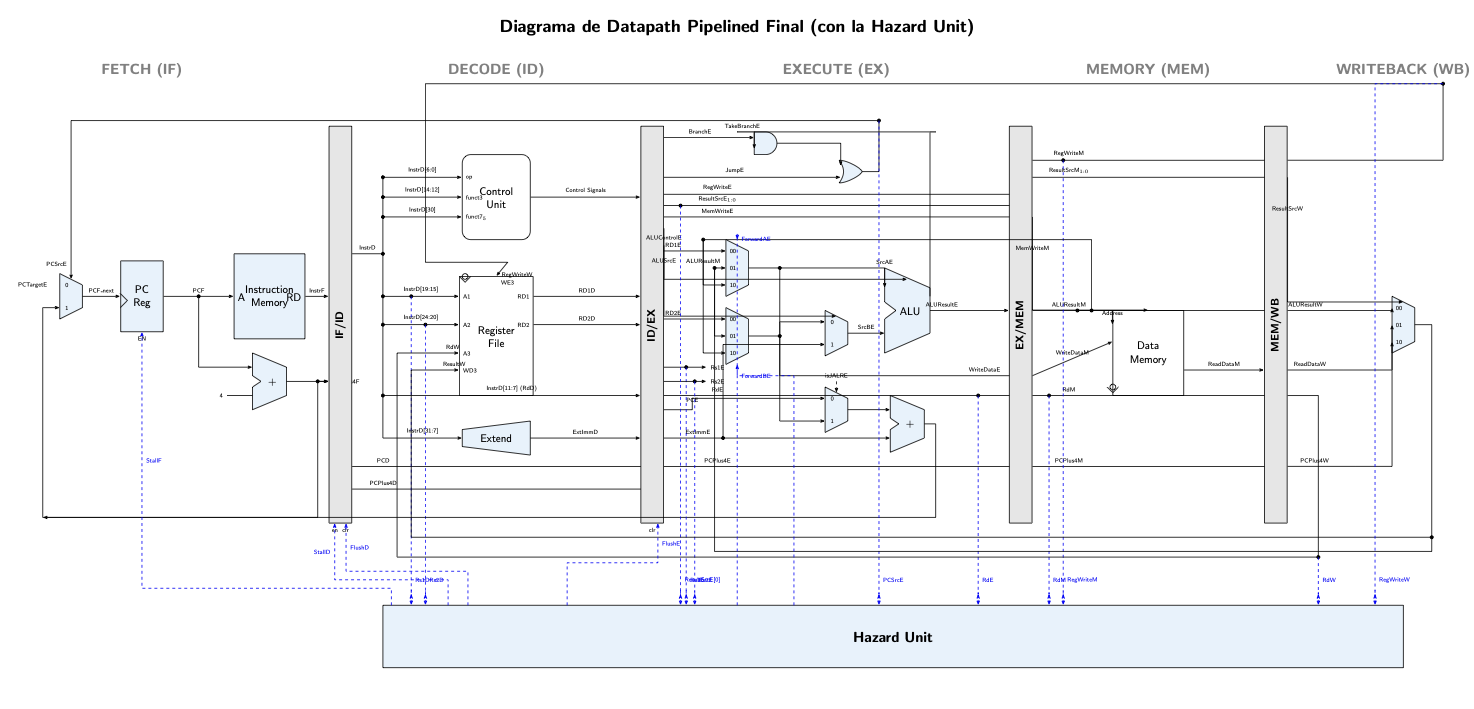
\includegraphics[width=\textwidth]{../Images/diagrama_final.png}
\caption{Diagrama del Datapath Pipelined completo del procesador (incluyendo la Hazard Unit).}
\end{figure}

El datapath final funciona correctamente ante cualquier dependencia de datos o de control debido a la incorporación de la Hazard Unit (unidad de control de riesgos) y los multiplexores de reenvío en la etapa Execute. La Hazard Unit supervisa continuamente y de forma combinacional los registros fuentes ($Rs1D$, $Rs2D$, $Rs1E$, $Rs2E$) y los compara con los registros de destino de instrucciones previas en las etapas de Execute ($RdE$), Memory ($RdM$) o Writeback ($RdW$) para tomar las siguientes acciones de control:
\begin{itemize}
    \item \textbf{Forwarding (Reenvío):} Si hay un riesgo de datos del tipo RAW (Read After Write), la unidad activa las señales de selección \texttt{ForwardAE} y/o \texttt{ForwardBE}. Esto hace que los multiplexores de 3 entradas ante la ALU tomen el dato más reciente desde Memory (\texttt{ALUResultM}) o Writeback (\texttt{ResultW}) en lugar de leer el valor obsoleto del banco de registros, logrando resolver el riesgo con 0 ciclos de penalización.
    \item \textbf{Stalling (Detección de Load-Use):} Cuando una instrucción de carga de memoria (\texttt{lw}) es seguida por otra que requiere su resultado en Execute, el reenvío no es suficiente ya que el dato se lee de memoria al final del ciclo de Memory. La unidad detecta esta condición y activa las señales de congelamiento \texttt{StallF} y \texttt{StallD} para detener la actualización del PC y del registro \texttt{IF/ID} por 1 ciclo, al mismo tiempo que activa \texttt{FlushE} para inyectar una burbuja (instrucción NOP) en la etapa Execute, permitiendo al \texttt{lw} obtener el dato y realizar el reenvío en el ciclo siguiente.
    \item \textbf{Flushing (Saltos Condicionales y Saltos Directos):} Si se determina que un salto es tomado en Execute (\texttt{PCSrcE = 1}), las instrucciones cargadas especulativamente en las etapas Fetch y Decode deben ser descartadas para evitar que se ejecuten. La Hazard Unit activa las señales \texttt{FlushD} y \texttt{FlushE} para borrar los registros \texttt{IF/ID} e \texttt{ID/EX} (convirtiéndolos en NOPs), perdiendo 2 ciclos de penalización pero garantizando la correcta ejecución del programa.
\end{itemize}


% ============================================================================
% SECCION 6: PROGRAMAS DE PRUEBA (1.0 pts)
% ============================================================================
\section{Programas de Prueba (CON Hazard Unit) (1.0 pts)}

Al activar la Hazard Unit real (\texttt{hunit.v}), los tres programas producen resultados correctos.

\subsection{Programa 2: Forwarding}

El programa prueba que la Hazard Unit detecta dependencias RAW y reenvía datos desde Memory y Writeback hacia Execute.

\begin{lstlisting}[style=pseudo, caption={Programa 2: test\_forwarding.mem}]
00: addi x2, x0, 5       // x2 = 5
04: addi x3, x0, 12      // x3 = 12
08: add  x4, x2, x3      // x4 = 5 + 12 = 17 (Forwarding)
0C: sw   x4, 200(x0)     // MEM[200] = 17
\end{lstlisting}

\begin{figure}[H]
\centering
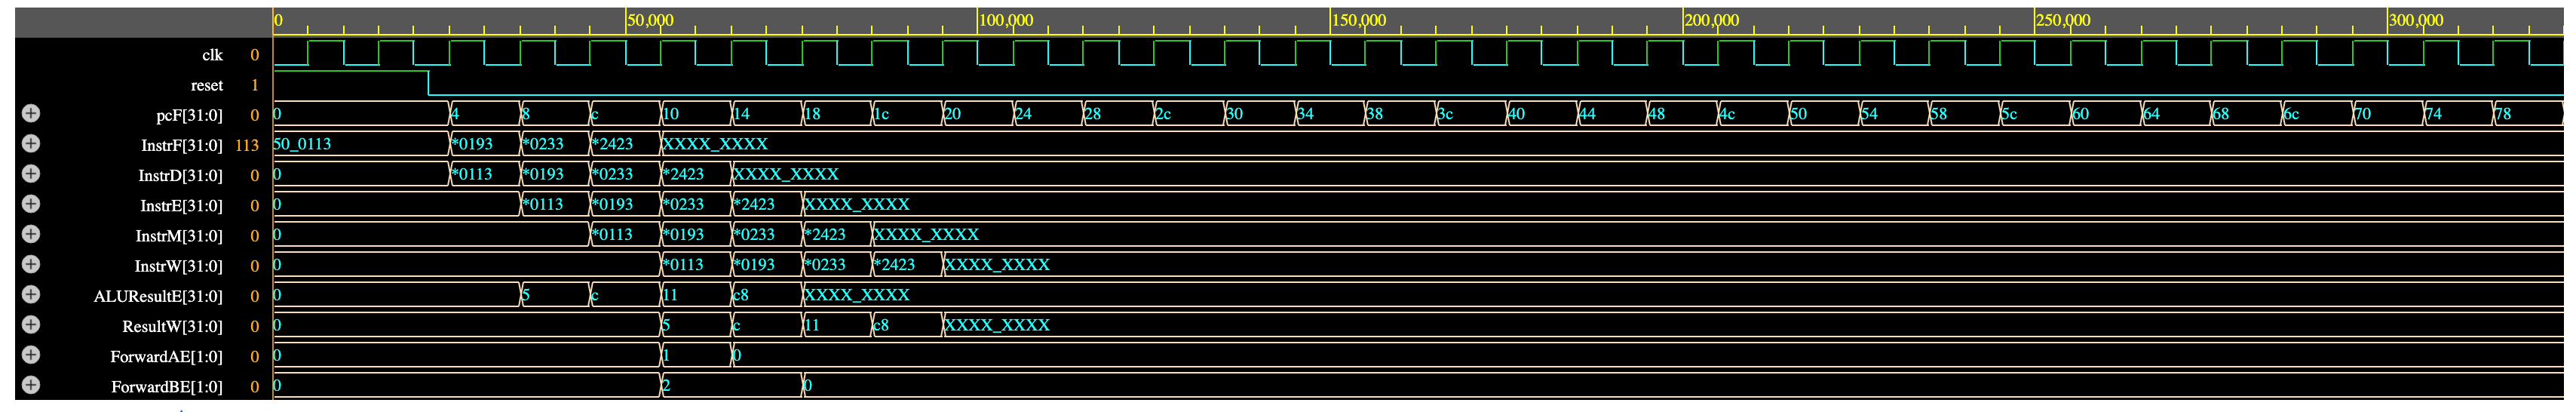
\includegraphics[width=0.90\textwidth]{../Images/waves_forwarding.png}
\caption{Programa 2 CON Hazard Unit. ForwardBE=10 reenvía x3 desde Memory; ForwardAE=01 reenvía x2 desde Writeback.}
\end{figure}

\textbf{Interpretación:} La Hazard Unit detecta que \texttt{x3} (recién calculado, en etapa Memory) y \texttt{x2} (en etapa Writeback) son necesarios por la instrucción \texttt{add x4, x2, x3}. Activa \texttt{ForwardBE=10} y \texttt{ForwardAE=01} para inyectar los valores correctos directamente a la ALU. El resultado es \texttt{0x11} (17 decimal), lo cual es correcto.

\subsection{Programa 3: Stalling}

El programa fuerza un Load-Use Hazard donde un \texttt{lw} es seguido inmediatamente por una instrucción que usa el dato cargado.

\begin{lstlisting}[style=pseudo, caption={Programa 3: test\_stalling.mem}]
00: addi x2, x0, 5       // x2 = 5
04: sw   x2, 100(x0)     // MEM[100] = 5
08: lw   x3, 100(x0)     // x3 = MEM[100] = 5
0C: add  x4, x3, x2      // STALL: x3 aun no esta listo
10: sw   x4, 200(x0)     // MEM[200] = 10
\end{lstlisting}

\begin{figure}[H]
\centering
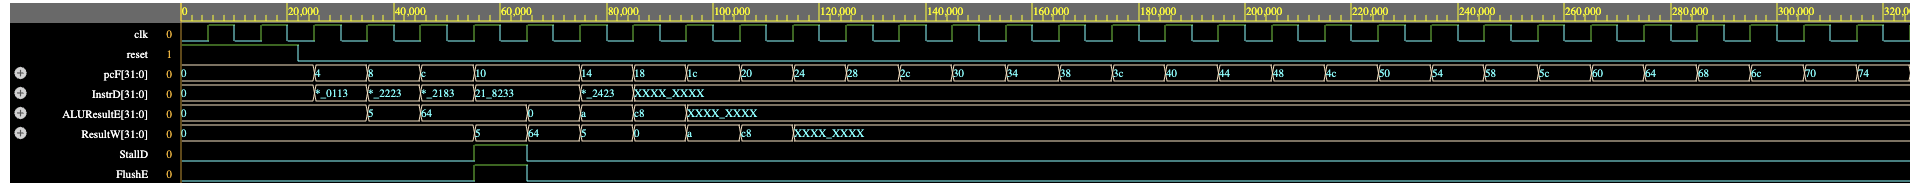
\includegraphics[width=0.92\textwidth]{../Images/waves_stalling.png}
\caption{Programa 3 CON Hazard Unit. StallD congela Decode y Fetch durante 1 ciclo; FlushE inserta una burbuja en Execute.}
\end{figure}

\textbf{Interpretación:} La Hazard Unit detecta que el \texttt{lw x3} está en Execute (aún no ha accedido a memoria) y la instrucción \texttt{add x4, x3, x2} en Decode necesita \texttt{x3}. Activa \texttt{StallD=1} y \texttt{StallF=1} congelando el PC y el registro IF/ID por 1 ciclo. Simultáneamente, \texttt{FlushE=1} inserta una burbuja NOP en Execute. Al ciclo siguiente, el dato ya está disponible y se reenvía vía forwarding.

\subsection{Programa 4: Flushing}

El programa fuerza un Control Hazard con un salto condicional (\texttt{beq}) que es tomado.

\begin{lstlisting}[style=pseudo, caption={Programa 4: test\_flushing.mem}]
00: addi x2, x0, 5       // x2 = 5
04: beq  x2, x2, 12      // Salta a línea 10 hex (siempre verdadero)
08: addi x3, x0, 1       // FLUSHED (no debe ejecutarse)
0C: addi x3, x0, 99      // FLUSHED (no debe ejecutarse)
10: add  x4, x0, x2      // x4 = 5 (destino del salto)
14: sw   x4, 200(x0)     // MEM[200] = 5
\end{lstlisting}

\begin{figure}[H]
\centering
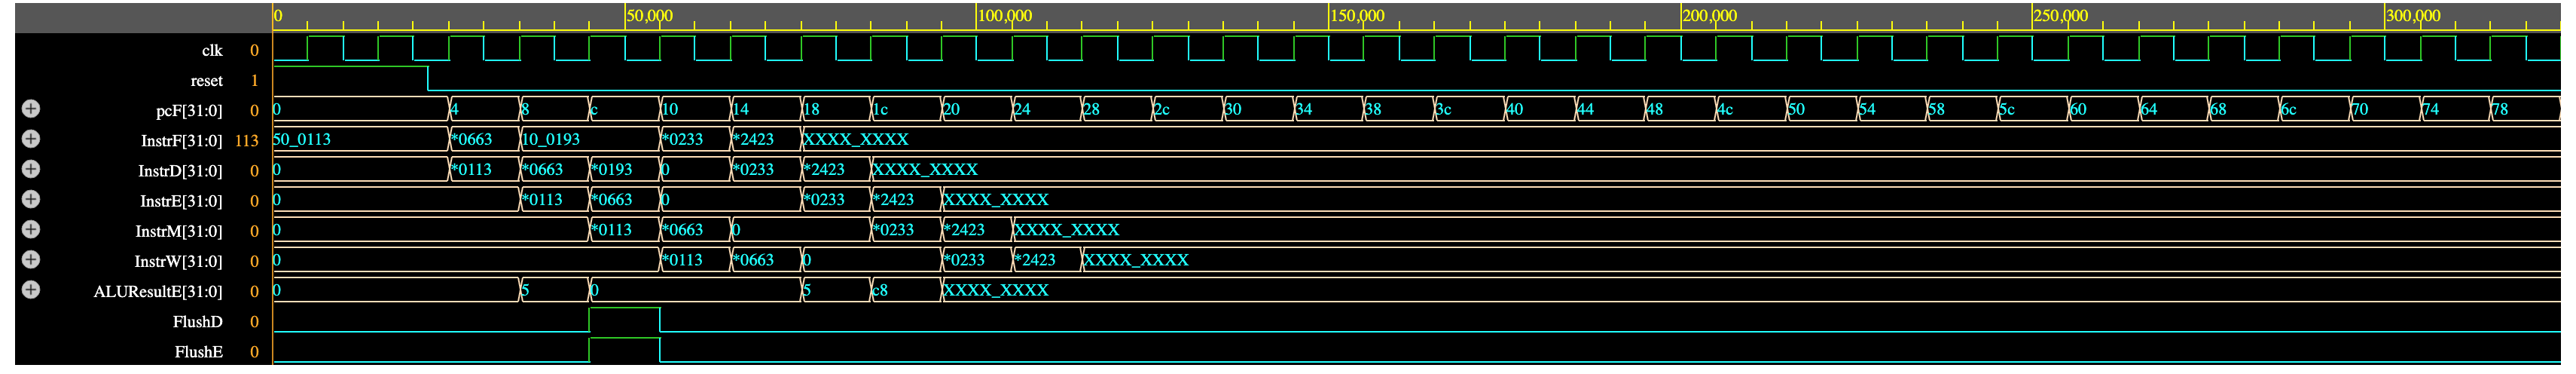
\includegraphics[width=0.86\textwidth]{../Images/waves_flushing.png}
\caption{Programa 4 CON Hazard Unit. FlushE y FlushD se activan cuando PCSrcE=1, descartando las instrucciones especulativas.}
\end{figure}

\textbf{Interpretación:} El \texttt{beq x2, x2} se resuelve en la etapa Execute (ciclo 3). La ALU confirma que \texttt{x2 == x2} y activa \texttt{PCSrcE=1}. La Hazard Unit responde activando \texttt{FlushD} y \texttt{FlushE}, convirtiendo las instrucciones especulativas (\texttt{addi x3, x0, 1} y \texttt{addi x3, x0, 99}) en burbujas NOP (\texttt{0x00000000}). El PC salta directamente a \texttt{0x10} y la ejecución continúa correctamente.

\subsection{Programa Extra: Set Completo de Operaciones y Validación de la ISA y Hazard Unit}

Para validar de forma integral el soporte de todas las operaciones de la ALU implementadas (incluyendo la red de inmediatos y desplazamientos) y todos los mecanismos de control (bifurcaciones condicionales y saltos incondicionales con flushing), se diseñó un programa adicional exhaustivo. Este programa ejecuta de manera consecutiva el repertorio RV32I completo, permitiendo visualizar riesgos de datos (RAW Hazards resueltos por reenvío) y riesgos de control (Control Hazards resueltos por vaciado de instrucciones).

\begin{lstlisting}[style=pseudo, caption={Programa Extra: test\_remaining\_ops.mem}]
00: addi x2, x0, 15  // x2 = 15 (0x0F)
04: addi x3, x0, 5   // x3 = 5
08: add  x4, x2, x3  // x4 = 15 + 5 = 20 (0x14) (RAW Hazard en x2 y x3 -> Forwarding)
0C: sub  x5, x2, x3  // x5 = 15 - 5 = 10 (0x0A) (RAW Hazard en x2 y x3 -> Forwarding)
10: and  x6, x2, x3  // x6 = 15 & 5 = 5 (0x05)
14: or   x7, x2, x3  // x7 = 15 | 5 = 15 (0x0F)
18: xor  x8, x2, x3  // x8 = 15 ^ 5 = 10 (0x0A)
1C: sll  x9, x2, x3  // x9 = 15 << 5 = 480 (0x1E0)
20: srl  x10, x2, x3 // x10 = 15 >> 5 = 0
24: sra  x11, x2, x3 // x11 = 15 >>> 5 = 0
28: slt  x12, x2, x3 // x12 = (15 < 5 signed) ? 1 : 0 = 0
2C: sltu x13, x2, x3 // x13 = (15 < 5 unsigned) ? 1 : 0 = 0
30: sw   x4, 100(x0) // Mem[100] = x4 = 20 (0x14) (RAW Hazard en x4 -> Forwarding)
34: lw   x14, 100(x0)// x14 = Mem[100] = 20 (0x14)
38: lui  x15, 0x12345// x15 = 0x12345000 (Carga de inmediato alto, U-type)
3C: slli x16, x14, 2 // x16 = 20 << 2 = 80 (0x50) (RAW Hazard en x14 -> Forwarding)
40: xori x17, x16, 10// x17 = 80 ^ 10 = 90 (0x5A) (RAW Hazard en x16 -> Forwarding)
44: srli x18, x16, 2 // x18 = 80 >> 2 = 20 (0x14) (RAW Hazard en x16)
48: srai x19, x16, 2 // x19 = 80 >>> 2 = 20 (0x14) (RAW Hazard en x16)
4C: ori  x20, x18, 5 // x20 = 20 | 5 = 21 (0x15) (RAW Hazard en x18)
50: andi x21, x18, 8 // x21 = 20 & 8 = 0 (0x00) (RAW Hazard en x18)
54: bne  x18, x19, 0x8C // no tomado (20 == 20). No altera el flujo del PC.
58: beq  x18, x19, 0x64 // tomado (20 == 20). Salta a 0x64. (Flushea 0x5C y 0x60)
5C: addi x5, x0, 99  // FLUSHED (burbuja NOP)
60: addi x5, x0, 99  // FLUSHED (burbuja NOP)
64: addi x22, x0, -10// x22 = -10 (0xfffffff6)
68: addi x23, x0, 5  // x23 = 5
6C: blt  x22, x23, 0x78 // tomado (-10 < 5, signed). Salta a 0x78. (Flushea 0x70 y 0x74)
70: addi x5, x0, 99  // FLUSHED
74: addi x5, x0, 99  // FLUSHED
78: bge  x23, x22, 0x84 // tomado (5 >= -10, signed). Salta a 0x84. (Flushea 0x7C y 0x80)
7C: addi x5, x0, 99  // FLUSHED
80: addi x5, x0, 99  // FLUSHED
84: jal  x1, 0x94    // Salto incondicional a 0x94. x1 = PC+4 = 0x88. (Flushea 0x88)
88: addi x5, x0, 99  // FLUSHED
8C: nop              // Trampa de error (no ejecutada)
90: nop              // Trampa de error (no ejecutada)
94: addi x24, x0, 172// x24 = 172 (0xAC)
98: jalr x25, x24, 0 // Salto indirecto a x24 + 0 = 0xAC. x25 = PC+4 = 0x9C. (Flushea 0x9C, 0xA0, 0xA4, 0xA8)
9C: addi x5, x0, 99  // FLUSHED
AC: addi x26, x0, 77 // x26 = 77 (0x4D) (Destino del salto indirecto JALR)
\end{lstlisting}

\begin{figure}[H]
\centering
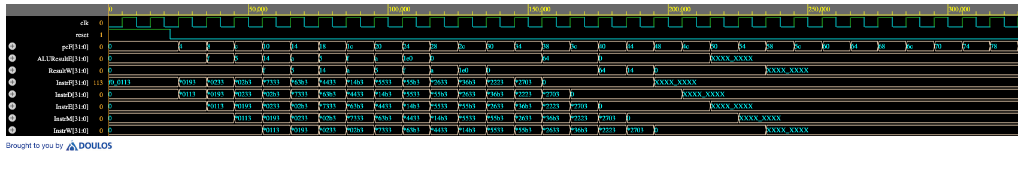
\includegraphics[width=0.95\textwidth]{../Images/waves_remaining_ops.png}
\caption{Formas de onda del Programa Extra. Se verifica el correcto comportamiento temporal y la resolución de dependencias de datos (forwarding) y de control (flushing) para todas las instrucciones RV32I.}
\end{figure}

\textbf{Interpretación:}
\begin{itemize}
  \item \textbf{Verificación de Operaciones ALU e Inmediatos}: Se valida la correcta ejecución de operaciones aritméticas con registro e inmediato. Por ejemplo:
    \begin{itemize}
      \item En el ciclo 16, la instrucción \texttt{slli} calcula \texttt{0x50} (80 decimal) a partir de \texttt{20} desplazado 2 bits.
      \item En el ciclo 17, la instrucción \texttt{xori} calcula \texttt{0x5A} (90 decimal) a partir de \texttt{80 \string^ 10}.
      \item La instrucción \texttt{lui} coloca el inmediato alto \texttt{0x12345000} en el registro \texttt{x15} (mostrado en \texttt{ResultW} en el ciclo 18).
    \end{itemize}
  \item \textbf{Control de Bifurcaciones (Branches)}:
    \begin{itemize}
      \item La instrucción \texttt{bne} en \texttt{0x54} no toma el salto al ser operandos iguales, permitiendo que el PC avance secuencialmente a \texttt{0x58}.
      \item La instrucción \texttt{beq} en \texttt{0x58} sí toma el salto, lo que provoca que \texttt{PCSrcE} se active, y la Hazard Unit aplique un \texttt{FlushD} y \texttt{FlushE} para limpiar las instrucciones especulativas en \texttt{0x5C} y \texttt{0x60}, saltando el PC directamente a \texttt{0x64}.
      \item Las instrucciones de branch comparativos con signo \texttt{blt} (menor que) y \texttt{bge} (mayor o igual) se evalúan correctamente, redirigiendo el PC a sus destinos con la consecuente inserción de burbujas en el pipeline.
    \end{itemize}
  \item \textbf{Saltos Incondicionales (`jal` y `jalr`)}:
    \begin{itemize}
      \item \texttt{jal} en \texttt{0x84} calcula su destino relativo en la etapa Execute y salta a \texttt{0x94}, guardando el enlace \texttt{PC+4 = 0x88} en \texttt{x1} en el ciclo 37.
      \item \texttt{jalr} en \texttt{0x98} calcula su destino basándose en el registro \texttt{x24} (que contiene \texttt{0xAC}), saltando directamente a la instrucción en \texttt{0xAC} (que carga \texttt{77} en \texttt{x26}) y guardando el enlace de retorno \texttt{PC+4 = 0x9C} en \texttt{x25} en el ciclo 41.
    \end{itemize}
\end{itemize}

% ============================================================================
% SECCION 7: EXTENSION RVC (16 BITS)
% ============================================================================
\section{Extension RVC (16-bits)}
La extension estandar RVC (Compressed Instructions) de la arquitectura RISC-V tiene como objetivo reducir el tamaño del código permitiendo que las instrucciones más frecuentes sean codificadas en 16 bits (2 bytes) en lugar de los 32 bits tradicionales.

\begin{figure}[H]
\centering
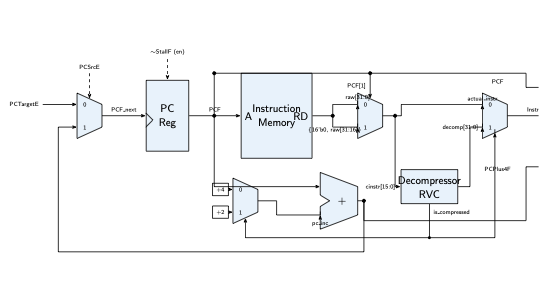
\includegraphics[width=0.95\textwidth]{../Images/Entrega2/diagrama_fetch_rvc.png}
\caption{Diagrama de hardware de la etapa de Fetch modificada para la extension RVC, mostrando la descompresión combinacional de 16 a 32 bits y el camino de incremento dinamico del PC hasta el registro de acoplamiento IF/ID.}
\label{fig:diagrama_fetch_rvc}
\end{figure}

\subsection{El Reto Arquitectonico y la Solucion}
En nuestro diseño original pipelined de 5 etapas, la CPU estaba diseñada asumiendo que el universo entero estaba hecho de bloques de 32 bits. Para no tener que reescribir todo el procesador (lo cual habria destruido la Hazard Unit), se adopto una solucion sumamente elegante: \textbf{ocultarle al pipeline que existen instrucciones de 16 bits}.

La meta fue crear un descompresor combinacional dentro de la primera etapa (Fetch). Cuando llega una instrucción de 16 bits, este traductor la convierte instantaneamente en su equivalente de 32 bits antes de que pase a la etapa Decode. Así, Decode siempre ve instrucciones estandar de 32 bits.


\subsection{Modificaciones al Código}
\begin{itemize}
    \item \textbf{Alineacion en Memoria:} Ahora la memoria se lee en bloques de 32 bits estandar, pero introducimos un multiplexor de hardware que revisa si el Program Counter esta desalineado (bit \texttt{PCF[1]}).
    \item \textbf{Descompresor (\texttt{decompressor.v}):} Este módulo extrae los 16 bits más bajos, revisa si es una instrucción comprimida, e infla los bits a su version RV32I.
    \item \textbf{El Engaño al Pipeline:} Se utiliza un multiplexor para elegir entre la instrucción leida original o la version expandida por el descompresor.
    \item \textbf{Avance Dinamico del PC:} El Program Counter ya no avanza 4 bytes rigidamente, sino que avanza $+2$ si la instrucción fue de 16 bits o $+4$ si fue de 32 bits.
\end{itemize}

\subsection{Justificacion: Unidad de Riesgos (Hazard Unit)}
Como parte de los requerimientos de diseño, es crucial justificar por que la Unidad de Riesgos (\texttt{hunit.v}) no requirio ninguna modificacion para soportar la extension RVC. 

La respuesta radica en la \textbf{estrategia de expansion en tiempo cero en la etapa de Fetch}. Al ubicar el módulo descompresor combinacional de RVC justo antes del registro de acoplamiento \texttt{IF/ID}, se logra un desacoplamiento completo (decoupling) entre la naturaleza de 16 bits de las instrucciones comprimidas y el resto del pipeline. 

A continuación se detallan las razones arquitectonicas y de control de esta decision:
\begin{enumerate}
    \item \textbf{Transparencia en Decode (ID):} Dado que la descompresión y alineacion ocurren en la etapa Fetch (IF), la instrucción que se escribe en el registro \texttt{IF/ID} y que posteriormente ingresa a la etapa Decode es siempre una instrucción RV32I estandar de 32 bits (\texttt{InstrD}). Por lo tanto, los puertos de lectura del banco de registros reciben las direcciones correctas de los registros fuente (\texttt{rs1} y \texttt{rs2}), y la Unidad de Control genera las señales de control estandar (ej. \texttt{RegWrite}, \texttt{MemtoReg}, \texttt{ALUControl}).
    \item \textbf{Deteccion Homogenea de Riesgos de Datos (RAW Hazards):} La Hazard Unit opera comparando las direcciones de los registros fuente de la instrucción en Decode (\texttt{Rs1D}, \texttt{Rs2D}) con las direcciones de los registros destino de las instrucciones previas en las etapas de Execute, Memory y Writeback (\texttt{RdE}, \texttt{RdM}, \texttt{RdW}). Como la instrucción en Decode ya ha sido inflada a 32 bits, los campos de registro se encuentran en las posiciones de bits estandar de RISC-V, permitiendo a la Hazard Unit detectar coincidencias y aplicar reenvio (forwarding) o detencion (stall) de manera totalmente transparente.
    \item \textbf{Manejo de Riesgos de Control (Control Hazards):} Ante saltos tomados (como \texttt{c.j}, \texttt{c.jal}, o branches comprimidos como \texttt{c.beqz}), el control se resuelve en la etapa Execute (EX) activando la señal \texttt{PCSrcE = 1}. Al igual que en la ISA base, la Hazard Unit responde activando \texttt{FlushD = 1} y \texttt{FlushE = 1} para vaciar las instrucciones especulativas en Fetch y Decode. El vaciado del pipeline escribe un NOP estandar (\texttt{0x00000013}) en los registros del pipeline, neutralizando cualquier instrucción sin importar si era de 16 o 32 bits originalmente.
    \item \textbf{Conservacion del Critical Path de Control:} La Hazard Unit suele estar en uno de los caminos criticos de temporizacion del procesador debido a la gran cantidad de comparaciones lógicas necesarias para forwarding. Mantenerla agnostica al tamaño de la instrucción evita añadir retardos adicionales en Decode/Execute, conservando la frecuencia maxima de reloj del procesador.
\end{enumerate}
En conclusión, el descompresor actua como un "filtro de traduccion" temprano en el pipeline. Esto permite que el resto del procesador, incluyendo la compleja Unidad de Riesgos, funcione como si estuviera ejecutando un programa RV32I puro, garantizando la correctitud y robustez del diseño.

\subsection{Código Verilog de la Extensión RVC}
A continuación se presenta el código Verilog correspondiente al módulo descompresor combinacional de 16 a 32 bits (\texttt{decompressor.v}). Este módulo es responsable de expandir en tiempo cero las instrucciones de 16 bits de la extensión RVC a sus equivalentes base de 32 bits (RV32I).

Para ver cómo se integra este módulo en la primera etapa del datapath, consúltese el código de la etapa Fetch en la Sección 2.5, que detalla la alineación de la instrucción en base al bit \texttt{PCF[1]}, la instanciación de este descompresor, el multiplexor final de selección de instrucción y el sumador con incremento dinámico del PC.

\begin{lstlisting}[style=verilogstyle, caption={Código Verilog del módulo descompresor RVC}]
module decompressor(
    input  logic [15:0] cinstr,    // Instrucción de 16-bits
    output logic [31:0] outstr,    // Instrucción expandida de 32-bits
    output logic        is_compressed // Bandera indicadora
);
    // Toda instrucción comprimida termina en 00, 01 o 10. (11 es 32-bits)
    assign is_compressed = (cinstr[1:0] != 2'b11);

    // ========================================================================
    // VARIABLES AUXILIARES (Extracción de campos RVC)
    // ========================================================================
    logic [4:0] rd_rs1;
    logic [4:0] rdp_rs1p; 
    logic [4:0] rs2p;     
    logic [4:0] rs2;

    // Variables para inmediatos
    logic [11:0] imm_addi;
    logic [19:0] imm_lui;
    logic [4:0]  shamt;
    
    // Nuevas variables para Memoria y Saltos
    logic [6:0]  imm_lw_sw;
    logic [7:0]  imm_lwsp;
    logic [7:0]  imm_swsp;
    logic [20:0] j_imm;
    logic [12:0] b_imm;

    // ========================================================================
    // ASIGNACIONES CONTINUAS (Desempaquetado de bits)
    // ========================================================================
    assign rd_rs1   = cinstr[11:7];
    assign rs2      = cinstr[6:2];
    assign rdp_rs1p = {2'b01, cinstr[9:7]}; // Sumar 8 para registros RVC (x8-x15)
    assign rs2p     = {2'b01, cinstr[4:2]}; // Sumar 8 para registros RVC (x8-x15)
    
    assign imm_addi = {{6{cinstr[12]}}, cinstr[12], cinstr[6:2]};
    assign imm_lui  = {{15{cinstr[12]}}, cinstr[6:2]};
    assign shamt    = {cinstr[12], cinstr[6:2]};

    // Immediatos de Memoria
    assign imm_lw_sw = {cinstr[5], cinstr[12:10], cinstr[6], 2'b00};
    assign imm_lwsp  = {cinstr[3:2], cinstr[12], cinstr[6:4], 2'b00};
    assign imm_swsp  = {cinstr[8:7], cinstr[12:9], 2'b00};

    // Immediatos de Saltos (J-Type y B-Type)
    assign j_imm = {{10{cinstr[12]}}, cinstr[8], cinstr[10:9], cinstr[6], cinstr[7], cinstr[2], cinstr[11], cinstr[5:3], 1'b0};
    assign b_imm = {{5{cinstr[12]}}, cinstr[6:5], cinstr[2], cinstr[11:10], cinstr[4:3], 1'b0};

    // ========================================================================
    // LÓGICA DE TRADUCCIÓN A 32-BITS
    // ========================================================================
    always_comb begin
        outstr = 32'h00000013; // Por defecto: NOP (addi x0, x0, 0)
        
        if (is_compressed) begin
            case (cinstr[1:0])
                // -----------------------------------------------------------
                // CUADRANTE 0 (Memoria basada en registros limitados)
                // -----------------------------------------------------------
                2'b00: begin 
                    case (cinstr[15:13])
                        3'b010: outstr = {5'b0, imm_lw_sw, rdp_rs1p, 3'b010, rs2p, 7'b0000011}; // c.lw
                        3'b110: outstr = {5'b0, imm_lw_sw[6:5], rs2p, rdp_rs1p, 3'b010, imm_lw_sw[4:0], 7'b0100011}; // c.sw
                    endcase
                end

                // -----------------------------------------------------------
                // CUADRANTE 1 (Aritmética, Saltos y Branches)
                // -----------------------------------------------------------
                2'b01: begin 
                    case (cinstr[15:13])
                        3'b000: outstr = {imm_addi, rd_rs1, 3'b000, rd_rs1, 7'b0010011}; // c.addi
                        3'b001: outstr = {j_imm[20], j_imm[10:1], j_imm[11], j_imm[19:12], 5'b00001, 7'b1101111}; // c.jal
                        3'b011: outstr = {imm_lui, rd_rs1, 7'b0110111};                  // c.lui
                        3'b100: begin // Grupo ALU
                            case (cinstr[11:10])
                                2'b00: outstr = {7'b0000000, shamt, rdp_rs1p, 3'b101, rdp_rs1p, 7'b0010011}; // c.srli
                                2'b01: outstr = {7'b0100000, shamt, rdp_rs1p, 3'b101, rdp_rs1p, 7'b0010011}; // c.srai
                                2'b10: outstr = {imm_addi, rdp_rs1p, 3'b111, rdp_rs1p, 7'b0010011};          // c.andi
                                2'b11: begin // Operaciones entre registros
                                    case (cinstr[6:5])
                                        2'b00: outstr = {7'b0100000, rs2p, rdp_rs1p, 3'b000, rdp_rs1p, 7'b0110011}; // c.sub
                                        2'b01: outstr = {7'b0000000, rs2p, rdp_rs1p, 3'b100, rdp_rs1p, 7'b0110011}; // c.xor
                                        2'b10: outstr = {7'b0000000, rs2p, rdp_rs1p, 3'b110, rdp_rs1p, 7'b0110011}; // c.or
                                        2'b11: outstr = {7'b0000000, rs2p, rdp_rs1p, 3'b111, rdp_rs1p, 7'b0110011}; // c.and
                                    endcase
                                end
                            endcase
                        end
                        3'b101: outstr = {j_imm[20], j_imm[10:1], j_imm[11], j_imm[19:12], 5'b00000, 7'b1101111}; // c.j
                        3'b110: outstr = {b_imm[12], b_imm[10:5], 5'b00000, rdp_rs1p, 3'b000, b_imm[4:1], b_imm[11], 7'b1100011}; // c.beqz
                        3'b111: outstr = {b_imm[12], b_imm[10:5], 5'b00000, rdp_rs1p, 3'b001, b_imm[4:1], b_imm[11], 7'b1100011}; // c.bnez
                    endcase
                end

                // -----------------------------------------------------------
                // CUADRANTE 2 (Memoria Stack Pointer y Registros completos)
                // -----------------------------------------------------------
                2'b10: begin 
                    case (cinstr[15:13])
                        3'b000: outstr = {7'b0000000, shamt, rd_rs1, 3'b001, rd_rs1, 7'b0010011}; // c.slli
                        3'b010: outstr = {4'b0, imm_lwsp, 5'd2, 3'b010, rd_rs1, 7'b0000011};      // c.lwsp
                        3'b100: begin
                            if (cinstr[12] == 0) begin
                                if (cinstr[6:2] == 0) outstr = {12'b0, rd_rs1, 3'b000, 5'b00000, 7'b1100111}; // c.jr
                                else                  outstr = {7'b0000000, rs2, rd_rs1, 3'b000, rd_rs1, 7'b0110011}; // c.add
                            end else begin
                                if (cinstr[6:2] == 0) outstr = {12'b0, rd_rs1, 3'b000, 5'b00001, 7'b1100111}; // c.jalr
                            end
                        end
                        3'b110: outstr = {4'b0, imm_swsp[7:5], rs2, 5'd2, 3'b010, imm_swsp[4:0], 7'b0100011}; // c.swsp
                    endcase
                end
            endcase
        end
    end
endmodule
\end{lstlisting}

\subsection{Explicacion Detallada de Cada Instruccion RVC (10 Instrucciones de la Parte 1)}
Para dar cumplimiento a los requerimientos de la Entrega 2, se presenta una explicacion del formato de 16 bits, el comportamiento y el codigo Verilog de descompresion asociado a cada una de las 10 instrucciones de la primera parte:

\begin{enumerate}
    \item \textbf{c.addi (c.addi rd, imm):}
    \begin{itemize}
        \item \textit{Funcionamiento:} Suma un inmediato de 6 bits con signo al valor del registro destino \texttt{rd} y almacena el resultado en \texttt{rd}.
        \item \textit{Mapeo RVC a RV32I:} Se expande a \texttt{addi rd, rd, imm}. El registro fuente \texttt{rs1} es identico al registro destino \texttt{rd} (\texttt{cinstr[11:7]}). El inmediato de 6 bits se forma combinando el bit de signo \texttt{cinstr[12]} y los bits \texttt{cinstr[6:2]}, y se extiende de signo a 12 bits.
        \item \textit{Codigo Verilog:}
        \begin{lstlisting}[style=verilogstyle]
assign imm_addi = {{6{cinstr[12]}}, cinstr[12], cinstr[6:2]};
// En case (cinstr[15:13]) -> 3'b000:
outstr = {imm_addi, rd_rs1, 3'b000, rd_rs1, 7'b0010011};
        \end{lstlisting}
    \end{itemize}

    \item \textbf{c.add (c.add rd, rs2):}
    \begin{itemize}
        \item \textit{Funcionamiento:} Suma el contenido de los registros \texttt{rd} y \texttt{rs2}, y guarda el resultado en \texttt{rd}.
        \item \textit{Mapeo RVC a RV32I:} Se expande a \texttt{add rd, rd, rs2}. Utiliza el registro completo de 5 bits para \texttt{rd/rs1} (\texttt{cinstr[11:7]}) y para \texttt{rs2} (\texttt{cinstr[6:2]}). La instruccion equivalente tiene funct7 = \texttt{0000000}, funct3 = \texttt{000} y opcode = \texttt{0110011}.
        \item \textit{Codigo Verilog:}
        \begin{lstlisting}[style=verilogstyle]
// En case (cinstr[15:13]) -> 3'b100: (con cinstr[12] == 0 y cinstr[6:2] != 0)
outstr = {7'b0000000, rs2, rd_rs1, 3'b000, rd_rs1, 7'b0110011};
        \end{lstlisting}
    \end{itemize}

    \item \textbf{c.sub (c.sub rd', rs2'):}
    \begin{itemize}
        \item \textit{Funcionamiento:} Resta el contenido del registro \texttt{rs2'} al del registro \texttt{rd'} y almacena el resultado en \texttt{rd'}.
        \item \textit{Mapeo RVC a RV32I:} Se expande a \texttt{sub rd', rd', rs2'}. Utiliza el rango de registros restringidos \texttt{x8-x15} (\texttt{rdp\_rs1p} y \texttt{rs2p}), decodificados a partir de 3 bits concatenando un prefijo constante \texttt{2'b01} en los bits mas significativos. La instruccion equivalente tiene funct7 = \texttt{0100000}, funct3 = \texttt{000} y opcode = \texttt{0110011}.
        \item \textit{Codigo Verilog:}
        \begin{lstlisting}[style=verilogstyle]
assign rdp_rs1p = {2'b01, cinstr[9:7]};
assign rs2p     = {2'b01, cinstr[4:2]};
// En case (cinstr[15:13]) -> 3'b100 -> case (cinstr[11:10]) -> 2'b11 -> case (cinstr[6:5]) -> 2'b00:
outstr = {7'b0100000, rs2p, rdp_rs1p, 3'b000, rdp_rs1p, 7'b0110011};
        \end{lstlisting}
    \end{itemize}

    \item \textbf{c.and (c.and rd', rs2'):}
    \begin{itemize}
        \item \textit{Funcionamiento:} Realiza un AND bit a bit entre los registros \texttt{rd'} y \texttt{rs2'}, y almacena el resultado en \texttt{rd'}.
        \item \textit{Mapeo RVC a RV32I:} Se expande a \texttt{and rd', rd', rs2'}. Utiliza operandos en registros restringidos \texttt{x8-x15}. La instruccion expandida posee funct7 = \texttt{0000000}, funct3 = \texttt{111} y opcode = \texttt{0110011}.
        \item \textit{Codigo Verilog:}
        \begin{lstlisting}[style=verilogstyle]
// En case (cinstr[15:13]) -> 3'b100 -> case (cinstr[11:10]) -> 2'b11 -> case (cinstr[6:5]) -> 2'b11:
outstr = {7'b0000000, rs2p, rdp_rs1p, 3'b111, rdp_rs1p, 7'b0110011};
        \end{lstlisting}
    \end{itemize}

    \item \textbf{c.or (c.or rd', rs2'):}
    \begin{itemize}
        \item \textit{Funcionamiento:} Realiza un OR bit a bit entre los registros \texttt{rd'} y \texttt{rs2'}, y almacena el resultado en \texttt{rd'}.
        \item \textit{Mapeo RVC a RV32I:} Se expande a \texttt{or rd', rd', rs2'}. Utiliza operandos en registros restringidos \texttt{x8-x15}. La instruccion equivalente tiene funct7 = \texttt{0000000}, funct3 = \texttt{110} y opcode = \texttt{0110011}.
        \item \textit{Codigo Verilog:}
        \begin{lstlisting}[style=verilogstyle]
// En case (cinstr[15:13]) -> 3'b100 -> case (cinstr[11:10]) -> 2'b11 -> case (cinstr[6:5]) -> 2'b10:
outstr = {7'b0000000, rs2p, rdp_rs1p, 3'b110, rdp_rs1p, 7'b0110011};
        \end{lstlisting}
    \end{itemize}

    \item \textbf{c.xor (c.xor rd', rs2'):}
    \begin{itemize}
        \item \textit{Funcionamiento:} Realiza un XOR bit a bit entre los registros \texttt{rd'} y \texttt{rs2'}, y almacena el resultado en \texttt{rd'}.
        \item \textit{Mapeo RVC a RV32I:} Se expande a \texttt{xor rd', rd', rs2'}. Utiliza operandos en registros restringidos \texttt{x8-x15}. La instruccion equivalente tiene funct7 = \texttt{0000000}, funct3 = \texttt{100} y opcode = \texttt{0110011}.
        \item \textit{Codigo Verilog:}
        \begin{lstlisting}[style=verilogstyle]
// En case (cinstr[15:13]) -> 3'b100 -> case (cinstr[11:10]) -> 2'b11 -> case (cinstr[6:5]) -> 2'b01:
outstr = {7'b0000000, rs2p, rdp_rs1p, 3'b100, rdp_rs1p, 7'b0110011};
        \end{lstlisting}
    \end{itemize}

    \item \textbf{c.slli (c.slli rd, shamt):}
    \begin{itemize}
        \item \textit{Funcionamiento:} Desplaza logicamente a la izquierda el registro destino \texttt{rd} segun el valor inmediato de desplazamiento \texttt{shamt}.
        \item \textit{Mapeo RVC a RV32I:} Se expande a \texttt{slli rd, rd, shamt}. Utiliza el registro completo de 5 bits \texttt{rd} (\texttt{cinstr[11:7]}). El valor de desplazamiento \texttt{shamt} es de 5 bits y se toma de \texttt{cinstr[6:2]}. En RV32C el bit \texttt{cinstr[12]} debe ser 0. La instruccion equivalente tiene funct7 = \texttt{0000000}, funct3 = \texttt{001} y opcode = \texttt{0010011}.
        \item \textit{Codigo Verilog:}
        \begin{lstlisting}[style=verilogstyle]
assign shamt = {cinstr[12], cinstr[6:2]}; // En RV32C cinstr[12] es 0, quedando de 5 bits
// En case (cinstr[15:13]) -> 3'b000 (en Cuadrante 2, cinstr[1:0] == 2'b10):
outstr = {7'b0000000, shamt, rd_rs1, 3'b001, rd_rs1, 7'b0010011};
        \end{lstlisting}
    \end{itemize}

    \item \textbf{c.srli (c.srli rd', shamt):}
    \begin{itemize}
        \item \textit{Funcionamiento:} Desplaza logicamente a la derecha el registro restringido \texttt{rd'} segun el valor inmediato de desplazamiento \texttt{shamt}.
        \item \textit{Mapeo RVC a RV32I:} Se expande a \texttt{srli rd', rd', shamt}. El registro destino y primer operando es el registro restringido \texttt{rd'} (\texttt{rdp\_rs1p}). El desplazamiento \texttt{shamt} es de 5 bits extraidos de \texttt{cinstr[6:2]}. La instruccion equivalente tiene funct7 = \texttt{0000000}, funct3 = \texttt{101} y opcode = \texttt{0010011}.
        \item \textit{Codigo Verilog:}
        \begin{lstlisting}[style=verilogstyle]
// En case (cinstr[15:13]) -> 3'b100 -> case (cinstr[11:10]) -> 2'b00:
outstr = {7'b0000000, shamt, rdp_rs1p, 3'b101, rdp_rs1p, 7'b0010011};
        \end{lstlisting}
    \end{itemize}

    \item \textbf{c.srai (c.srai rd', shamt):}
    \begin{itemize}
        \item \textit{Funcionamiento:} Desplaza aritmeticamente a la derecha el registro restringido \texttt{rd'} segun el valor inmediato \texttt{shamt} (conservando el bit de signo).
        \item \textit{Mapeo RVC a RV32I:} Se expande a \texttt{srai rd', rd', shamt}. El registro afectado es el restringido \texttt{rd'} (\texttt{rdp\_rs1p}). El \texttt{shamt} es de 5 bits de \texttt{cinstr[6:2]}. La instruccion equivalente requiere funct7 = \texttt{0100000} (indicando desplazamiento aritmetico), funct3 = \texttt{101} y opcode = \texttt{0010011}.
        \item \textit{Codigo Verilog:}
        \begin{lstlisting}[style=verilogstyle]
// En case (cinstr[15:13]) -> 3'b100 -> case (cinstr[11:10]) -> 2'b01:
outstr = {7'b0100000, shamt, rdp_rs1p, 3'b101, rdp_rs1p, 7'b0010011};
        \end{lstlisting}
    \end{itemize}

    \item \textbf{c.lui (c.lui rd, nzimm):}
    \begin{itemize}
        \item \textit{Funcionamiento:} Carga un inmediato no nulo de 6 bits desplazado a la izquierda por 12 bits en el registro destino \texttt{rd}.
        \item \textit{Mapeo RVC a RV32I:} Se expande a \texttt{lui rd, nzimm}. El registro destino es \texttt{rd} (\texttt{cinstr[11:7]}), el cual no puede ser ni \texttt{x0} ni \texttt{x2} (SP). El inmediato superior de 20 bits se forma extendiendo de signo el bit \texttt{cinstr[12]} por 15 bits a la izquierda y concatenando los 5 bits \texttt{cinstr[6:2]}. Opcode de la instruccion es \texttt{0110111}.
        \item \textit{Codigo Verilog:}
        \begin{lstlisting}[style=verilogstyle]
assign imm_lui  = {{15{cinstr[12]}}, cinstr[6:2]};
// En case (cinstr[15:13]) -> 3'b011:
outstr = {imm_lui, rd_rs1, 7'b0110111};
        \end{lstlisting}
    \end{itemize}
\end{enumerate}

\subsection{Cambios en el Datapath para la Adaptacion de RVC}
Para soportar la extension comprimida, se implementaron cambios clave en el datapath de la etapa Fetch (\texttt{fetch.v}), detallados y justificados a continuacion junto con sus fragmentos de codigo Verilog correspondientes:

\begin{enumerate}
    \item \textbf{Logica de Alineacion a Media Palabra (Half-Word Alignment Mux):}
    \begin{itemize}
        \item \textit{Descripcion:} Dado que la memoria de instrucciones original lee en bloques alineados a 4 bytes, pero las instrucciones comprimidas de 16 bits provocan que las instrucciones puedan comenzar en una direccion impar de media palabra (ej. \texttt{0x02}, \texttt{0x06}), se agrego un multiplexor que detecta si el PC actual apunta a una direccion desalineada mediante el bit \texttt{PCF[1]}.
        \item \textit{Codigo del Cambio:}
        \begin{lstlisting}[style=verilogstyle]
// Si PCF[1] == 1, la instruccion util empieza en los bits superiores [31:16]
assign actual_instr = PCF[1] ? {16'b0, raw_imem_data[31:16]} : raw_imem_data;
        \end{lstlisting}
    \end{itemize}

    \item \textbf{Integracion del Modulo de Descompresion y Multiplexor de Seleccion (Zero-Time Expansion):}
    \begin{itemize}
        \item \textit{Descripcion:} Se extrae la media palabra inferior de la instruccion alineada y se pasa por el modulo combinacional \texttt{decompressor}. Luego, un multiplexor final selecciona entre la instruccion de 32 bits original o la instruccion descomprimida.
        \item \textit{Codigo del Cambio:}
        \begin{lstlisting}[style=verilogstyle]
assign cinstr = actual_instr[15:0];

decompressor decomp (
  .cinstr(cinstr),
  .outstr(decompressed_instr),
  .is_compressed(is_compressed)
);

// Mux final de seleccion de instruccion
assign InstrF = is_compressed ? decompressed_instr : actual_instr;
        \end{lstlisting}
    \end{itemize}

    \item \textbf{Incremento Dinamico del PC:}
    \begin{itemize}
        \item \textit{Descripcion:} Para que el PC avance secuencialmente la cantidad correcta de bytes, ya no se incrementa rigidamente en $+4$. Si la instruccion actual es de 16 bits, el PC avanza $+2$ bytes; de lo contrario, avanza $+4$ bytes.
        \item \textit{Codigo del Cambio:}
        \begin{lstlisting}[style=verilogstyle]
assign pc_increment = is_compressed ? 32'd2 : 32'd4;

adder pcadd (
  .a(PCF),
  .b(pc_increment),
  .y(PCPlus4F)
);
        \end{lstlisting}
    \end{itemize}
\end{enumerate}


\subsection{Pruebas de la Extension RVC}

\subsubsection{Test RVC Básico (\texttt{test\_rvc\_basic.mem})}
El test básico tiene como finalidad comprobar que la lógica de descompresión combinacional y el calculo dinamico de incremento del PC funcionan de manera integrada en el pipeline para flujos de instrucciones mixtas (16 y 32 bits). El programa ejecuta la siguiente secuencia de operaciones:

\begin{lstlisting}[style=pseudo, caption={Programa RVC Básico: test\_rvc\_basic.mem}]
0x00: c.addi x8, 5         // x8 = 5 (Arithmetic immediate addition)
0x02: c.addi x9, 10        // x9 = 10 (Arithmetic immediate addition)
0x04: add    x10, x8, x9   // x10 = x8 + x9 = 15 (Normal 32-bit arithmetic)
0x08: c.sub  x8, x9        // x8 = x8 - x9 = -5 (ALU register-register subtract)
0x0A: c.j    skip          // Jump of 4 bytes forward (Unconditional Jump)
0x0C: nop                  // NOP (Bypassed/flushed, never committed)
0x10: addi   x11, x0, 100  // x11 = 100 (Normal 32-bit addition, destination)
\end{lstlisting}

\renewcommand{\thefigure}{18.\arabic{figure}}
\renewcommand{\theHfigure}{18.\arabic{figure}}
\setcounter{figure}{0}

\begin{figure}[H]
\centering
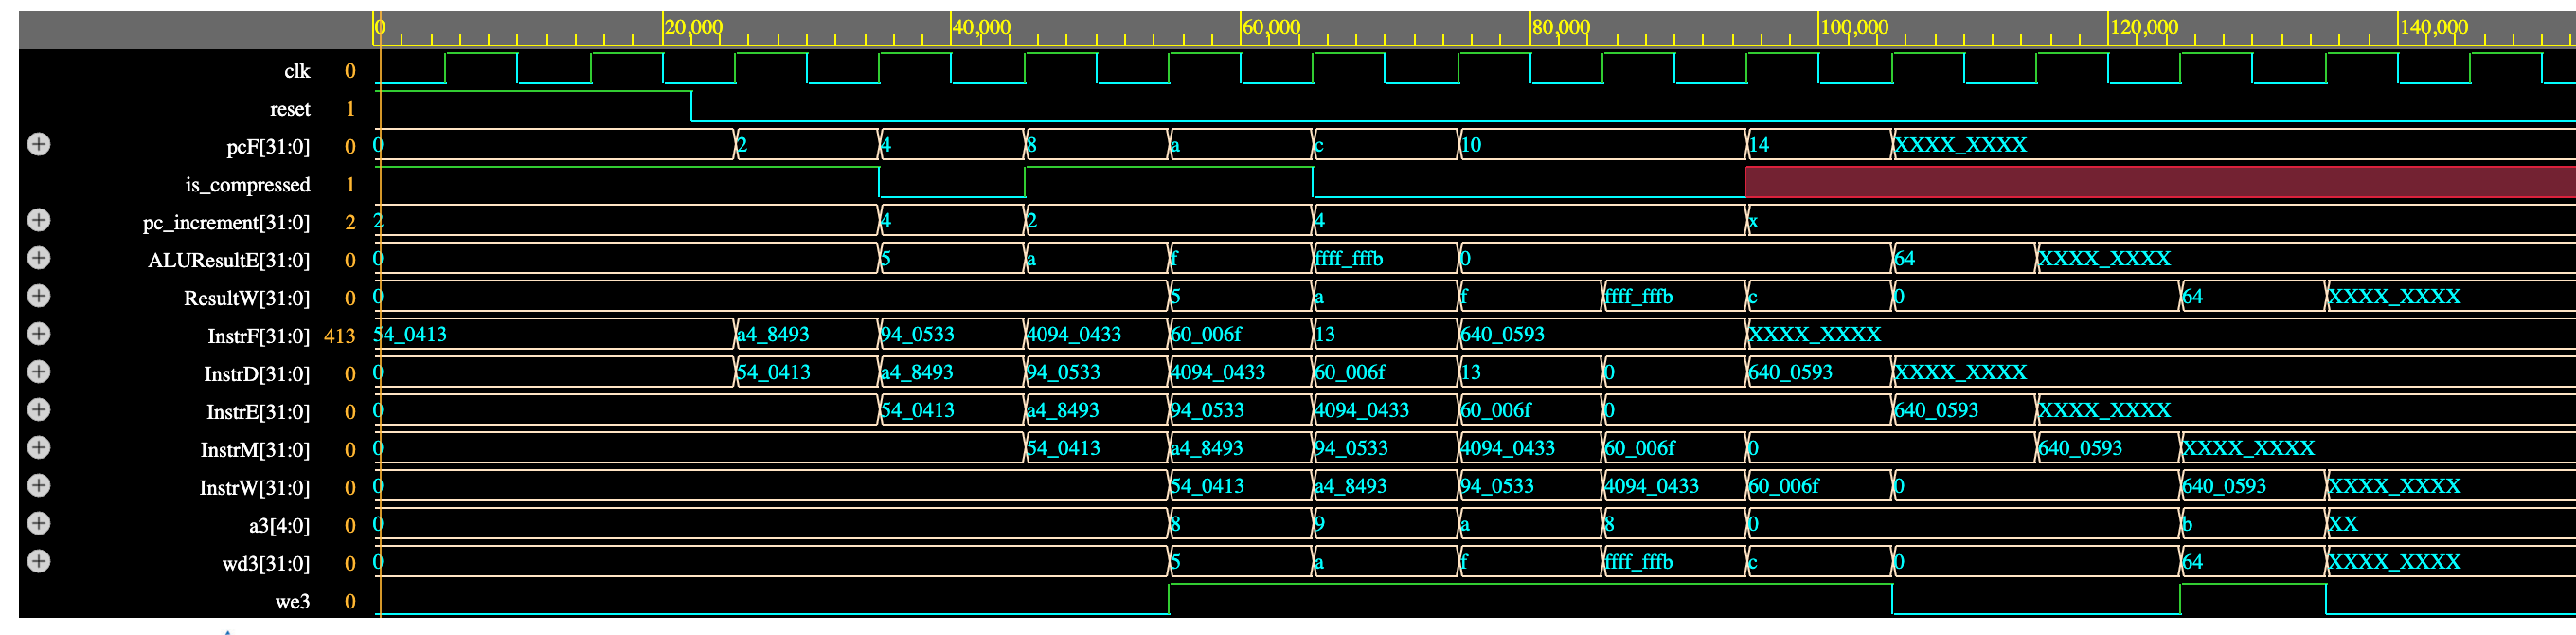
\includegraphics[width=0.95\textwidth]{../Images/Entrega2/waves_rvc_basic/waves_rvc_basic.png}
\caption{Forma de onda general del test básico RVC, mostrando el avance completo del programa desde la salida de reset hasta la escritura final.}
\label{fig:waves_rvc_basic_general}
\end{figure}

\begin{figure}[H]
\centering
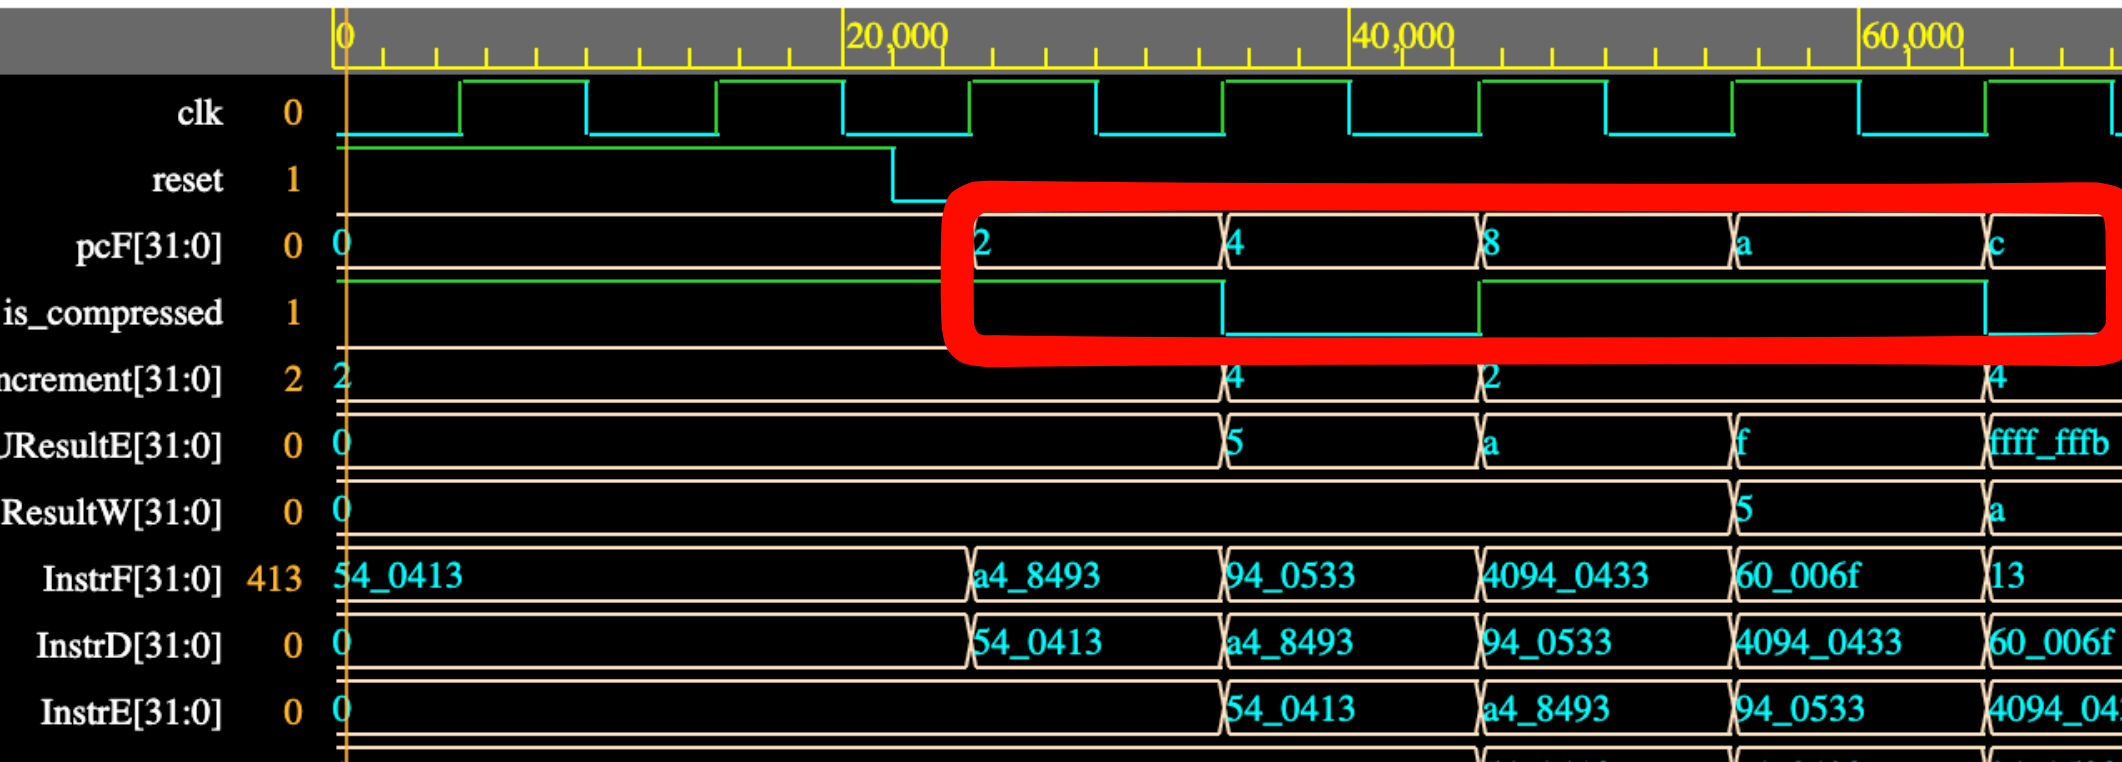
\includegraphics[width=0.95\textwidth]{../Images/Entrega2/waves_rvc_basic/waves_rvc_basic_e1.png}
\caption{Incremento Dinamico}
\label{fig:waves_rvc_basic_e1}
\end{figure}

\textbf{Incremento Dinamico:}
En la forma de onda de la Fig. \ref{fig:waves_rvc_basic_e1}, se visualiza la respuesta dinamica del PC en Fetch ante instrucciones mixtas. 
\begin{itemize}
  \item En el ciclo donde \texttt{PCF = 0x00}, la instrucción leida es comprimida. La señal interna \texttt{is\_compressed} se eleva a \texttt{1} y el incremento \texttt{pc\_increment} se calcula como \texttt{2}. Esto causa que en el siguiente ciclo el PC avance a \texttt{0x02}.
  \item En el ciclo de \texttt{PCF = 0x02}, la instrucción sigue siendo comprimida (mitad superior de la palabra leida). \texttt{is\_compressed} sigue en \texttt{1} y \texttt{pc\_increment} en \texttt{2}, avanzando el PC en el siguiente ciclo a \texttt{0x04}.
  \item En el ciclo de \texttt{PCF = 0x04}, se lee la instrucción de 32 bits \texttt{add}. El descompresor detecta los bits de control \texttt{11} en los bits menos significativos, por lo que \texttt{is\_compressed} cae a \texttt{0} y el incremento \texttt{pc\_increment} cambia automaticamente a \texttt{4}, enviando el PC en el ciclo siguiente a \texttt{0x08}.
\end{itemize}
Esto demuestra el perfecto control dinamico de incremento del PC por hardware en la etapa Fetch.

\begin{figure}[H]
\centering
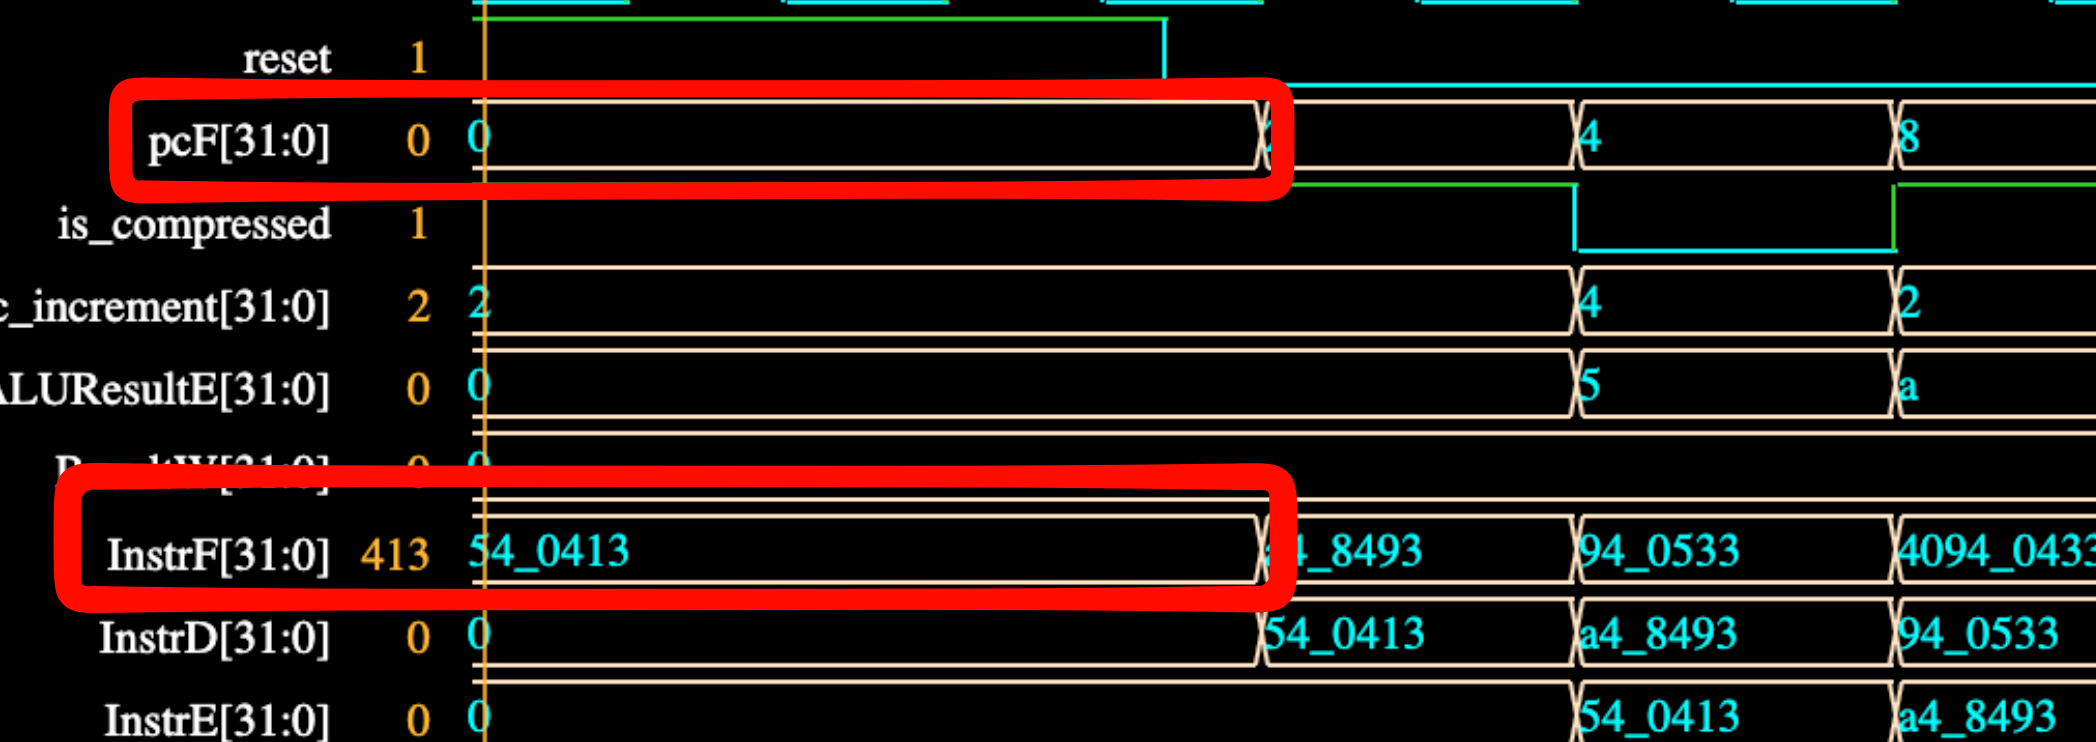
\includegraphics[width=0.95\textwidth]{../Images/Entrega2/waves_rvc_basic/waves_rvc_basic_e2.png}
\caption{Descompresión en Fetch}
\label{fig:waves_rvc_basic_e2}
\end{figure}

\textbf{Descompresión en Fetch:}
En la Fig. \ref{fig:waves_rvc_basic_e2}, se comprueba la traduccion de instrucciones comprimidas. En el ciclo 1, el PC apunta a \texttt{0x00}. La memoria entrega la palabra \texttt{raw\_imem\_data = 0x04A90415}.
\begin{itemize}
  \item Dado que \texttt{PCF[1] = 0}, la instrucción actual alineada a media palabra es \texttt{0x0415} (\texttt{c.addi x8, 5}).
  \item El descompresor combinacional analiza los bits de esta instrucción y, de manera instantanea y en el mismo ciclo, coloca en el bus \texttt{InstrF} el valor \texttt{0x00540413}, que es la codificacion estandar de 32 bits de la instrucción \texttt{addi x8, x8, 5}.
\end{itemize}
Como el hardware traduce la instrucción antes de registrarla en el buffer \texttt{IF/ID}, la etapa Decode (\texttt{InstrD}) solo ve instrucciones estandar de 32 bits, evitando tener que propagar la complejidad de RVC en las etapas posteriores del pipeline.

\begin{figure}[H]
\centering
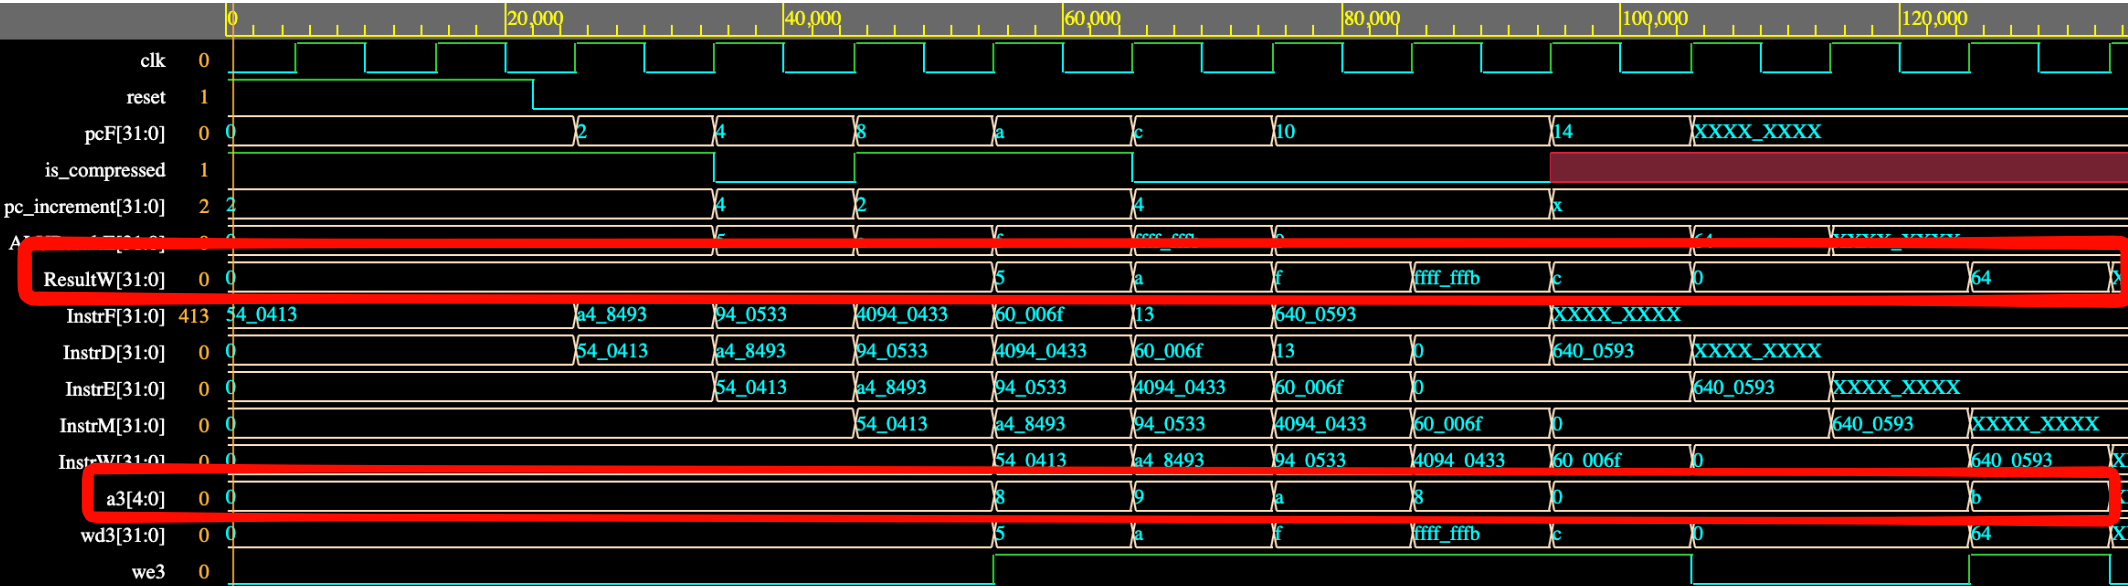
\includegraphics[width=0.95\textwidth]{../Images/Entrega2/waves_rvc_basic/waves_rvc_basic_e3.png}
\caption{Escritura y Salto}
\label{fig:waves_rvc_basic_e3}
\end{figure}

\textbf{Escritura y Salto:}
La Fig. \ref{fig:waves_rvc_basic_e3} muestra la escritura secuencial de los resultados en el banco de registros a traves de \texttt{ResultW} y los registros correspondientes en la etapa Writeback (WB):
\begin{itemize}
  \item El registro \texttt{x8} se escribe con \texttt{5}.
  \item El registro \texttt{x9} se escribe con \texttt{10} (\texttt{0x0A} en hex).
  \item El registro \texttt{x10} recibe la suma de ambos registros, escribiendo \texttt{15} (\texttt{0x0F} en hex).
  \item La instrucción \texttt{c.sub x8, x9} en \texttt{0x08} escribe \texttt{-5} (\texttt{0xFFFFFFFB} o \texttt{*fb} en GTKWave) en el registro \texttt{x8}.
  \item La instrucción \texttt{c.j skip} en \texttt{0x0A} realiza un salto incondicional directo hacia la etiqueta \texttt{skip} (\texttt{0x10}), lo que causa que la instrucción \texttt{nop} en la dirección \texttt{0x0C} sea descartada en Fetch y no altere ningun registro.
  \item El programa aterriza en \texttt{skip} (\texttt{0x10}), escribiendo el valor final \texttt{100} (\texttt{0x64} en hex) en el registro \texttt{x11}.
\end{itemize}
Esto valida la correcta ejecución e integridad de los datos en toda la arquitectura del procesador.

\subsubsection{Test RVC de Memoria (\texttt{test\_rvc\_memory.mem})}
El test de memoria tiene como finalidad validar que las instrucciones de carga y almacenamiento comprimidas (\texttt{c.lw} y \texttt{c.sw}) interactuan de manera correcta con la memoria de datos de 32 bits a traves de las etapas del pipeline. El programa ejecuta la siguiente secuencia de instrucciones:

\begin{lstlisting}[style=pseudo, caption={Programa RVC Memoria: test\_rvc\_memory.mem}]
0x00: addi x8, x0, 0       // x8 = 0 (Base register initialized)
0x04: addi x9, x0, 42      // x9 = 42 (Register value to write)
0x08: c.sw x9, 4(x8)       // Store x9 to address x8+4 (0xC044, 16-bit)
0x0A: c.lw x10, 4(x8)      // Load x10 from address x8+4 (0x4048, 16-bit)
0x0C: nop                  // NOP
\end{lstlisting}

\renewcommand{\thefigure}{19.\arabic{figure}}
\renewcommand{\theHfigure}{19.\arabic{figure}}
\setcounter{figure}{0}

\begin{figure}[H]
\centering
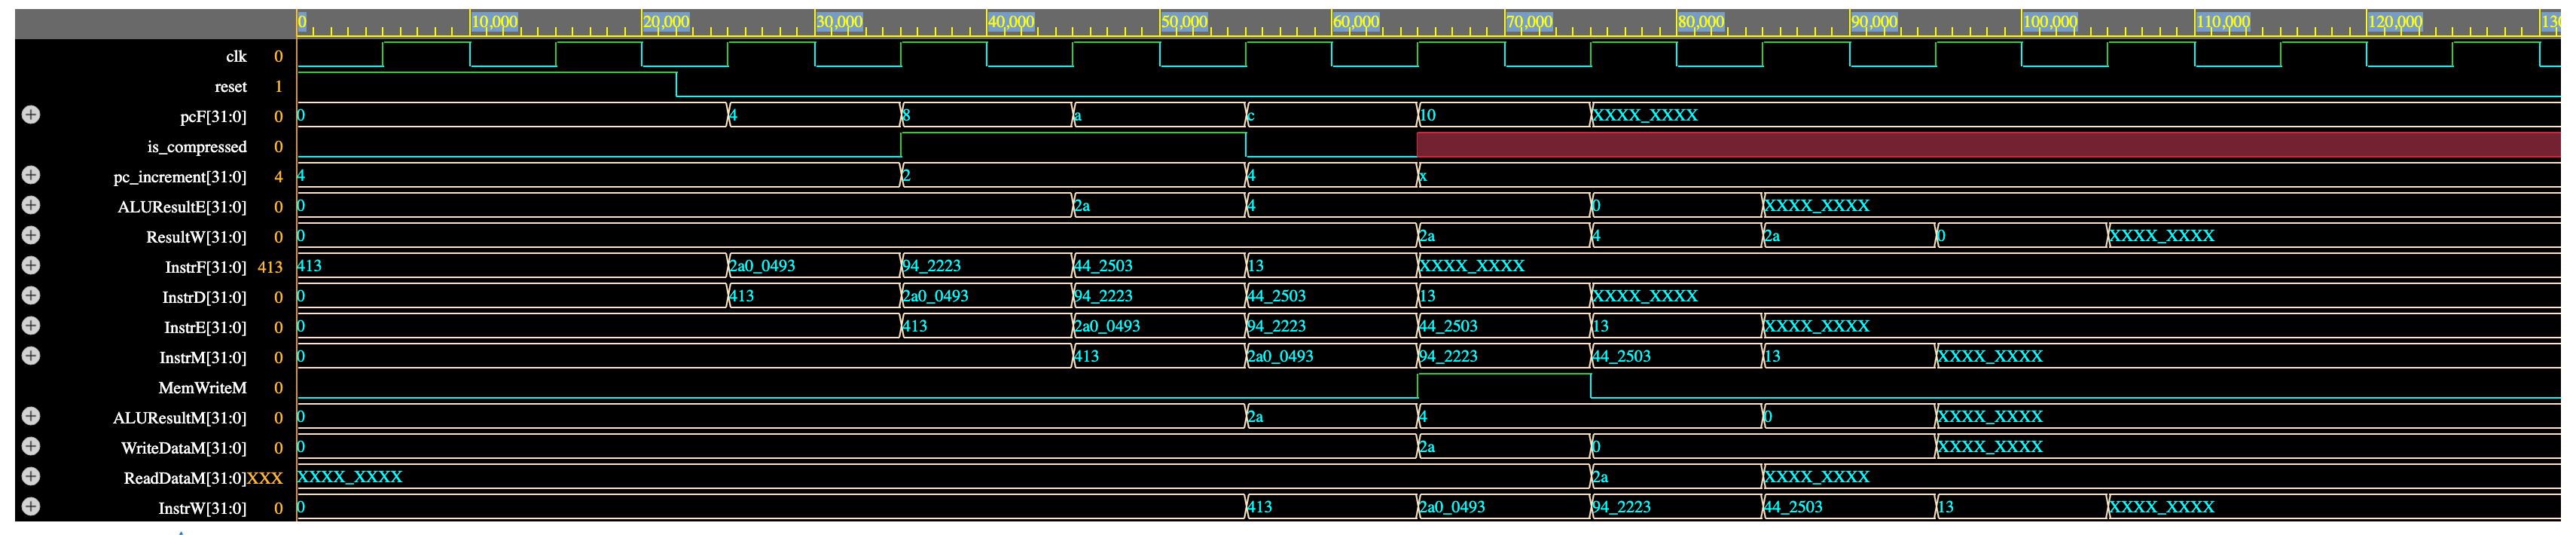
\includegraphics[width=0.95\textwidth]{../Images/Entrega2/waves_rvc_memory/waves_rvc_memory.png}
\caption{Forma de onda general del test de memoria RVC, validando la ruta completa de carga y almacenamiento de datos.}
\label{fig:waves_rvc_memory_general}
\end{figure}

\begin{figure}[H]
\centering
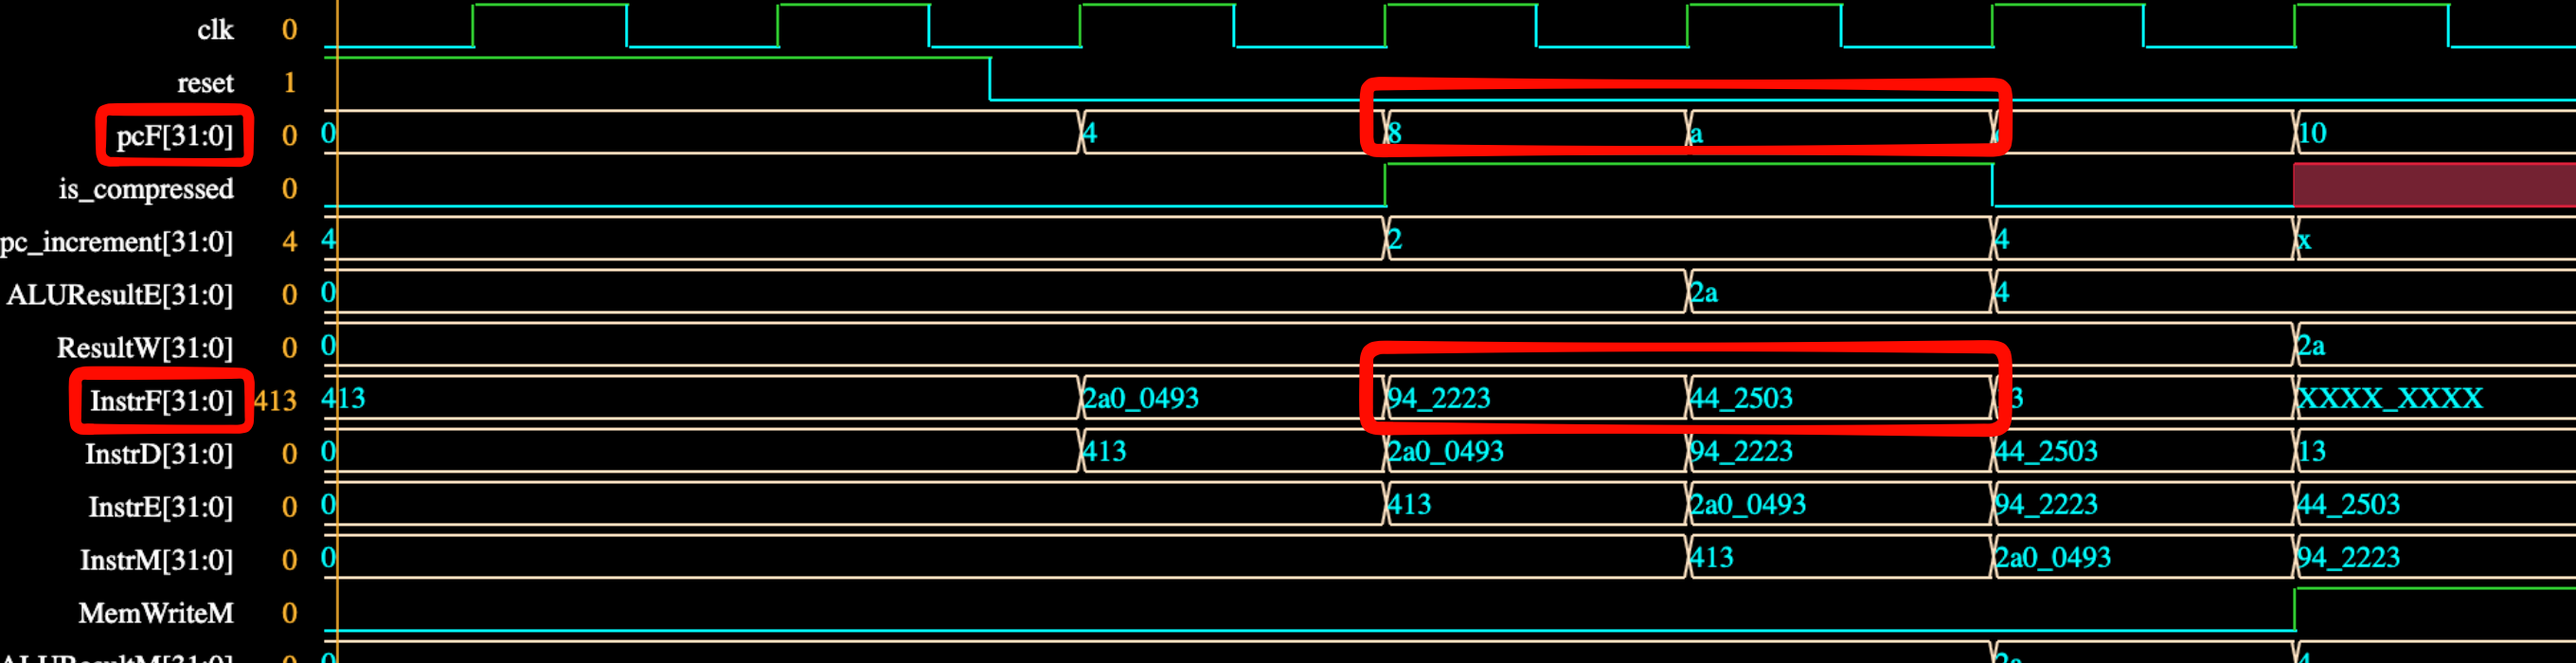
\includegraphics[width=0.95\textwidth]{../Images/Entrega2/waves_rvc_memory/waves_rvc_memory_e1.png}
\caption{Descompresión de Memorias}
\label{fig:waves_rvc_memory_e1}
\end{figure}

\textbf{Descompresión de Memorias:}
En la forma de onda de la Fig. \ref{fig:waves_rvc_memory_e1}:
Enmarca la señal \texttt{pcF} avanzando de \texttt{0x08} a \texttt{0x0A}, y muestra que la instrucción comprimida \texttt{0xC044} se expande en tiempo real en la etapa Fetch a la instrucción de 32 bits \texttt{0x00942223} (\texttt{sw x9, 4(x8)}). De igual forma, en \texttt{pcF = 0x0A}, la instrucción comprimida \texttt{0x4048} se expande a la instrucción de 32 bits \texttt{0x00442503} (\texttt{lw x10, 4(x8)}).
\\
En la etapa Fetch, se visualiza el incremento de PC de 2 en 2 bytes (\texttt{0x08} a \texttt{0x0A}). Al estar en \texttt{pcF = 0x08}, la instrucción comprimida \texttt{0xC044} se expande instantaneamente a la instrucción de 32 bits \texttt{0x00942223} (\texttt{sw}). En \texttt{pcF = 0x0A}, la instrucción \texttt{0x4048} se expande a \texttt{0x00442503} (\texttt{lw}).

\begin{figure}[H]
\centering
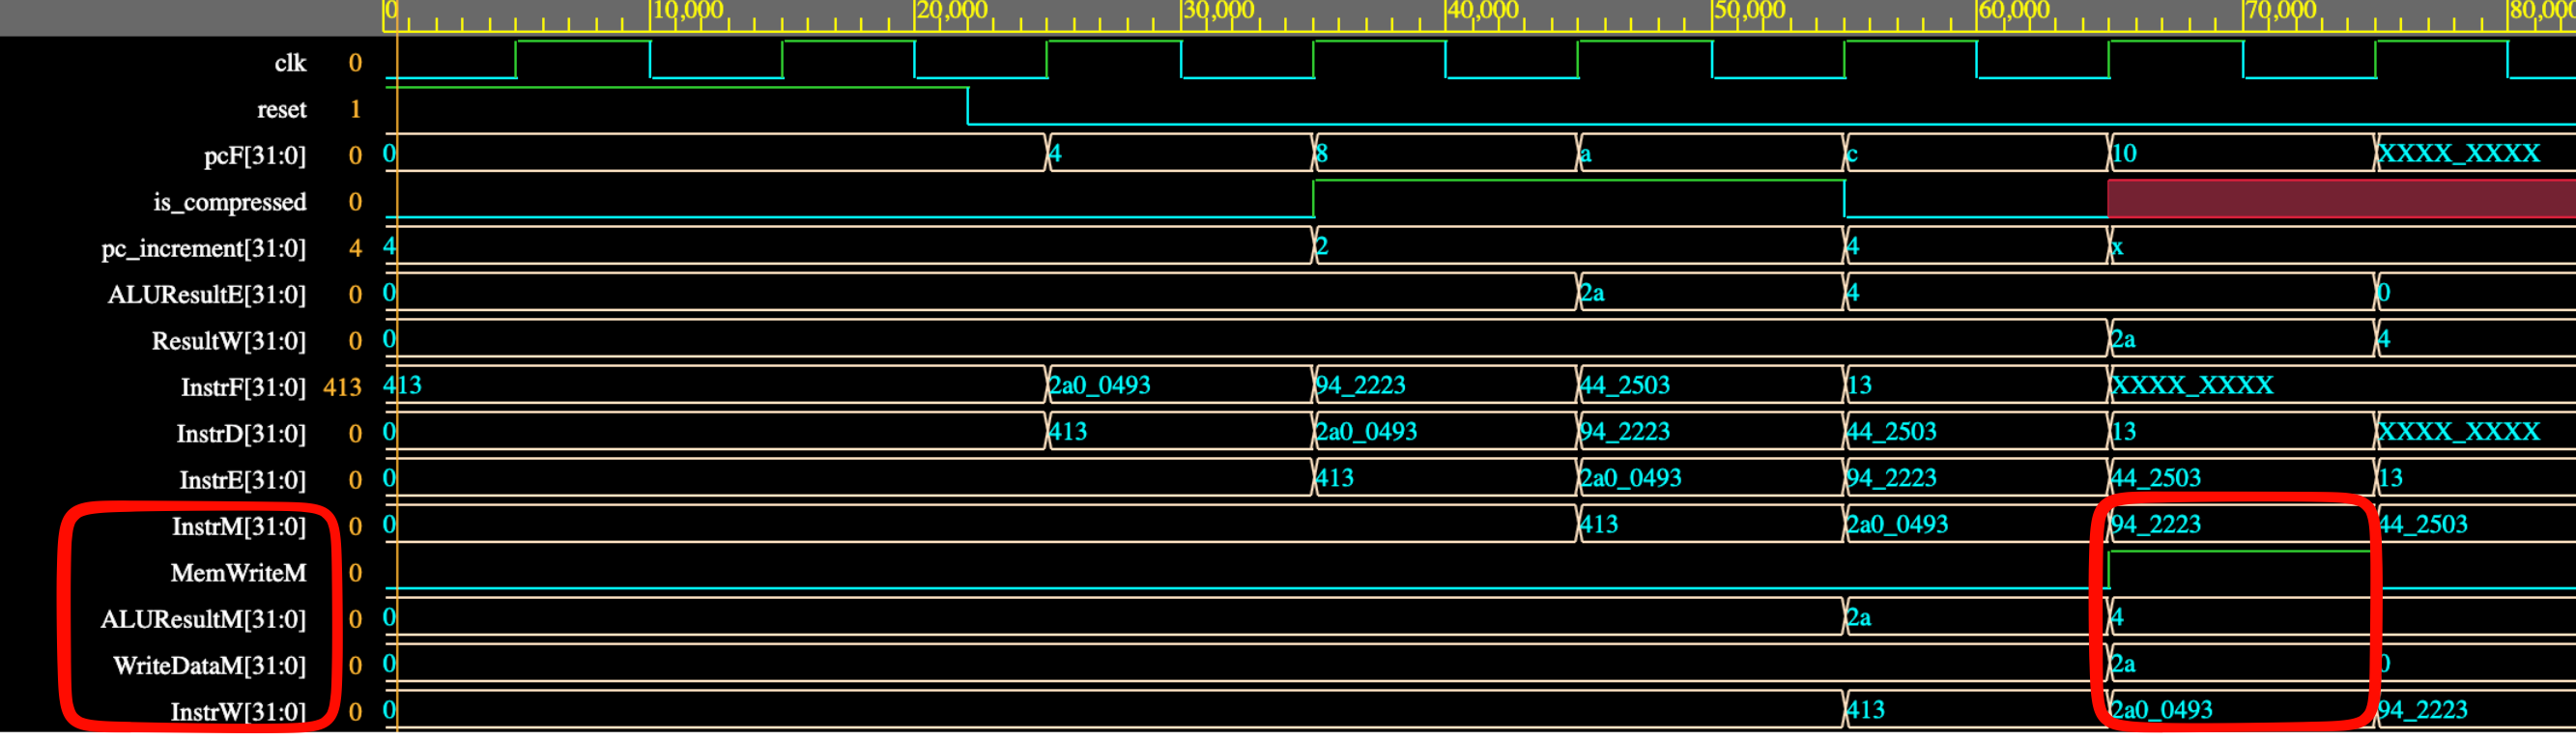
\includegraphics[width=0.95\textwidth]{../Images/Entrega2/waves_rvc_memory/waves_rvc_memory_e2.png}
\caption{Escritura en Memoria (Store)}
\label{fig:waves_rvc_memory_e2}
\end{figure}

\textbf{Escritura en Memoria (Store):}
En la forma de onda de la Fig. \ref{fig:waves_rvc_memory_e2}:
Enmarca la etapa Memory (\texttt{InstrM = 0x00942223}) donde la señal de habilitacion de escritura de la memoria de datos \texttt{MemWriteM} se activa en alto (\texttt{1}). Muestra que la dirección calculada es \texttt{ALUResultM = 4} y el bus de datos a escribir \texttt{WriteDataM} toma el valor \texttt{2a} (42 en decimal).
\\
Cuando la instrucción de escritura llega a la etapa Memory (\texttt{InstrM = 0x00942223}), la señal de habilitacion de escritura de la memoria de datos \texttt{MemWriteM} se activa en alto (\texttt{1}). La dirección de destino calculada por la ALU es \texttt{ALUResultM = 4} (dirección base $0 + 4 = 4$) y el bus de datos a escribir \texttt{WriteDataM} toma el valor \texttt{2a} (42 en decimal).

\begin{figure}[H]
\centering
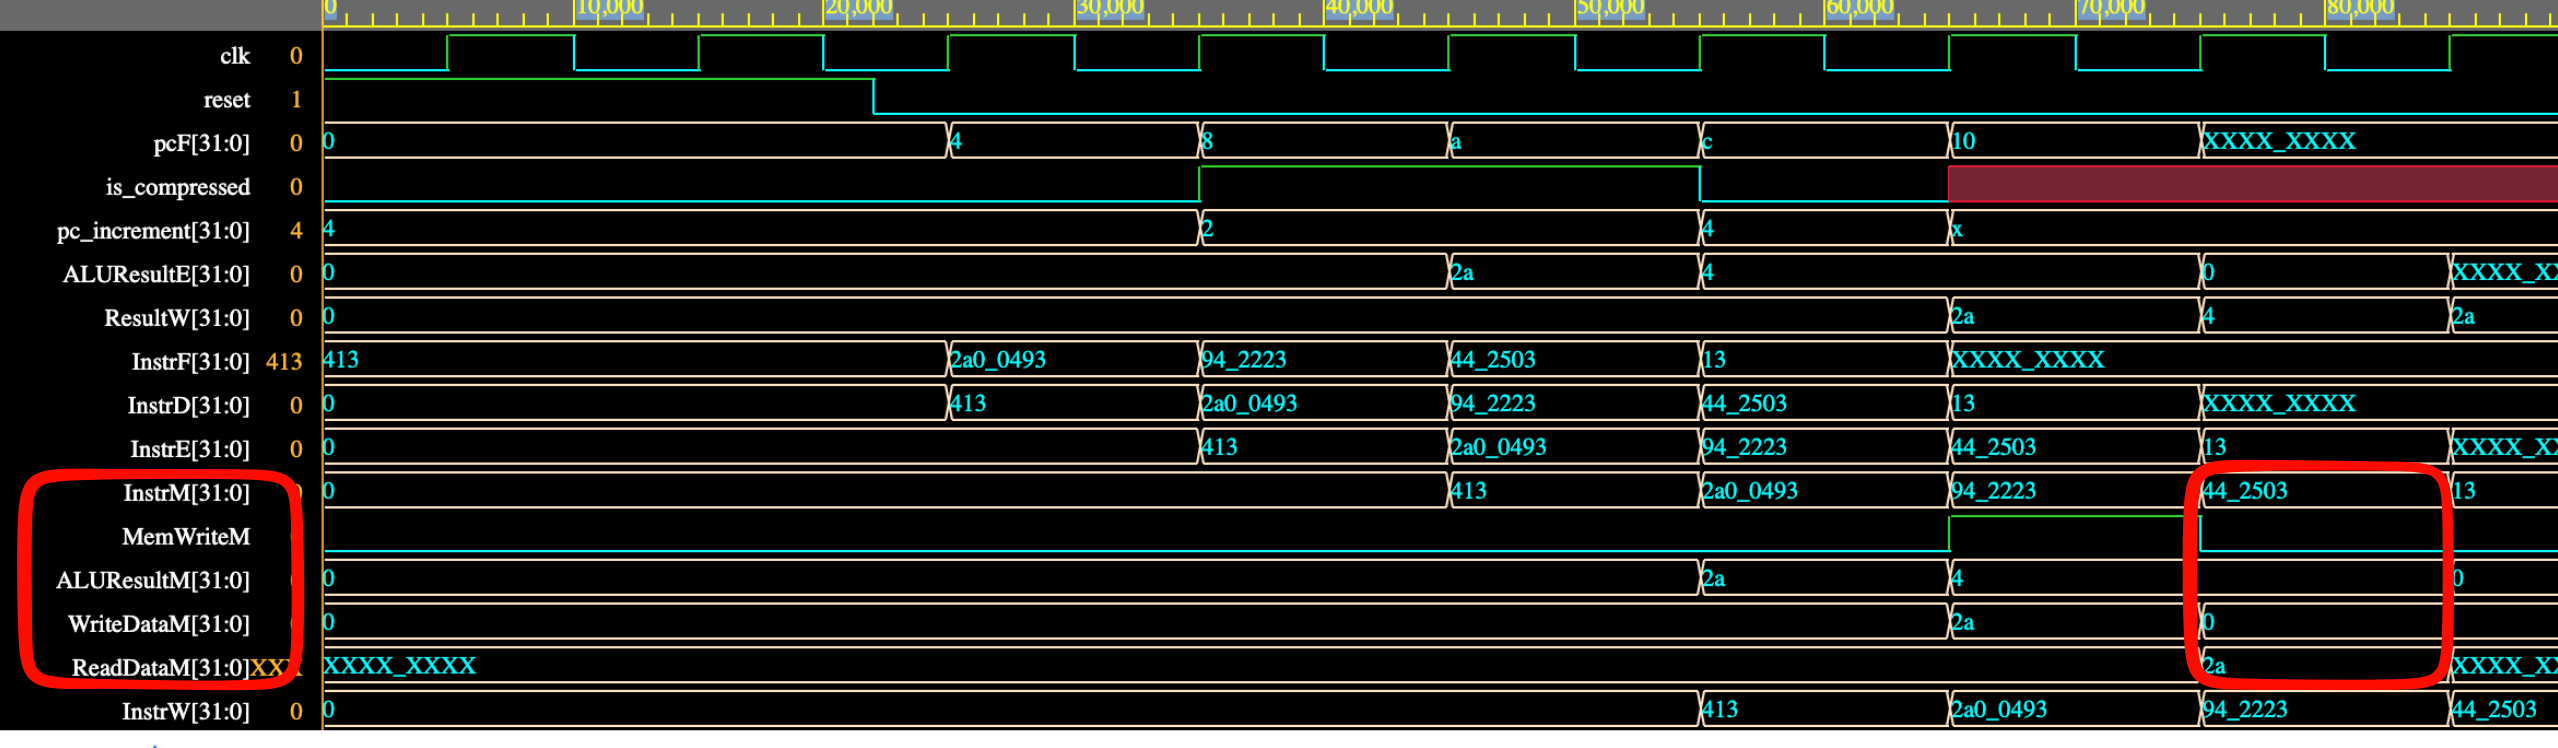
\includegraphics[width=0.95\textwidth]{../Images/Entrega2/waves_rvc_memory/waves_rvc_memory_e3.png}
\caption{Lectura de Memoria (Load)}
\label{fig:waves_rvc_memory_e3}
\end{figure}

\textbf{Lectura de Memoria (Load):}
En la forma de onda de la Fig. \ref{fig:waves_rvc_memory_e3}:
Enmarca la etapa Memory para la instrucción de carga (\texttt{InstrM = 0x00442503}), mostrando que la señal de control de escritura \texttt{MemWriteM} se mantiene en bajo (\texttt{0}) para realizar la lectura. Muestra que la dirección solicitada es \texttt{ALUResultM = 4} y que el bus de lectura de datos de la memoria entrega el valor de 32 bits \texttt{2a} (42 en decimal).
\\
Cuando la instrucción de carga llega a la etapa Memory (\texttt{InstrM = 0x00442503}), la señal \texttt{MemWriteM} se desactiva en bajo (\texttt{0}) para realizar la lectura. La dirección a leer es \texttt{ALUResultM = 4}, retornando el dato de 32 bits \texttt{2a} (42 en decimal) almacenado en la RAM.

\begin{figure}[H]
\centering
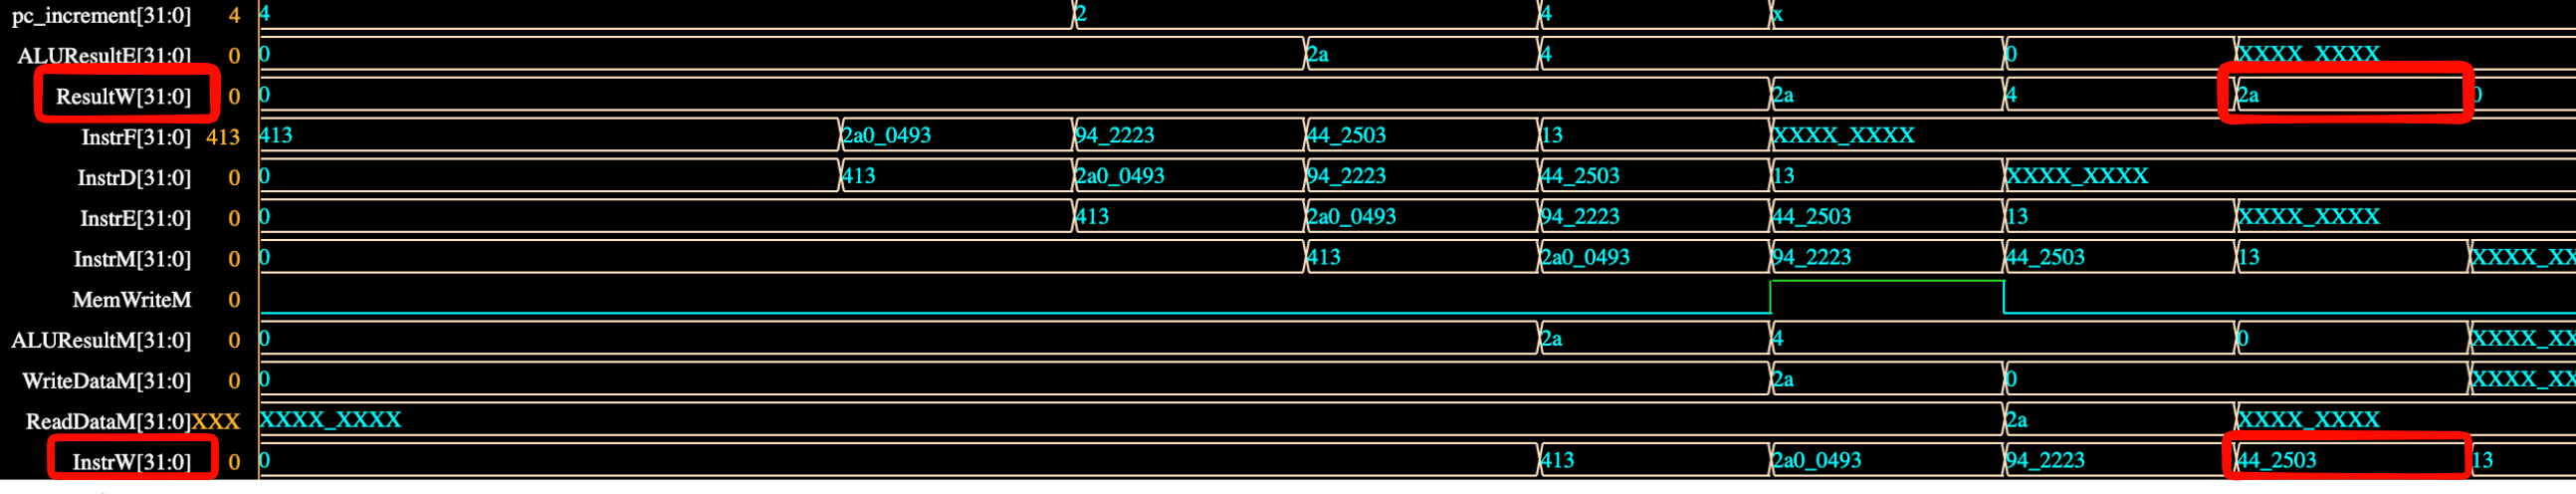
\includegraphics[width=0.95\textwidth]{../Images/Entrega2/waves_rvc_memory/waves_rvc_memory_e4.png}
\caption{Escritura Final en el Registro}
\label{fig:waves_rvc_memory_e4}
\end{figure}

\textbf{Escritura Final en el Registro:}
En la forma de onda de la Fig. \ref{fig:waves_rvc_memory_e4}:
Enmarca la señal \texttt{ResultW[31:0]} mostrando el valor \texttt{2a} (42 en decimal) en el bus de escritura al registro en la etapa Writeback (WB), y la señal \texttt{InstrW} mostrando el valor \texttt{00442503} (que representa la instrucción \texttt{lw x10, 4(x8)}).
\\
Cuando la instrucción de carga llega a la etapa Writeback (WB) (\texttt{InstrW = 0x00442503}), la señal \texttt{ResultW} escribe el valor de datos de retorno \texttt{2a} (42 en decimal) en el registro destino del banco de registros, completando la operación exitosamente.
Esto demuestra que el procesador segmentado soporta accesos de lectura y escritura alineados a media palabra desde instrucciones comprimidas de manera transparente.


\subsubsection{Test RVC de Saltos (\texttt{test\_rvc\_branches.mem})}
El test de saltos condicionales tiene como finalidad evaluar el comportamiento del camino de control y la resolución de bifurcaciones comprimidas, verificando el calculo del destino y el vaciado del pipeline ante un salto tomado. El programa ejecuta la siguiente secuencia de instrucciones:

\begin{lstlisting}[style=pseudo, caption={Programa RVC Saltos: test\_rvc\_branches.mem}]
0x00: addi   x8, x0, 0     // x8 = 0 (Base register initialized)
0x04: addi   x9, x0, 1     // x9 = 1 (Conditional register initialized)
0x08: c.beqz x9, 4         // Branch if x9 == 0 to 0x0C (Not taken, PC+2)
0x0A: c.bnez x9, 4         // Branch if x9 != 0 to 0x0C (Taken, PC+2 -> PC corrected)
0x0C: nop                  // NOP (Bypassed/flushed, never committed)
0x10: addi   x10, x0, 99   // x10 = 99 (Branch target instruction executed)
\end{lstlisting}

\renewcommand{\thefigure}{20.\arabic{figure}}
\renewcommand{\theHfigure}{20.\arabic{figure}}
\setcounter{figure}{0}

\begin{figure}[H]
\centering
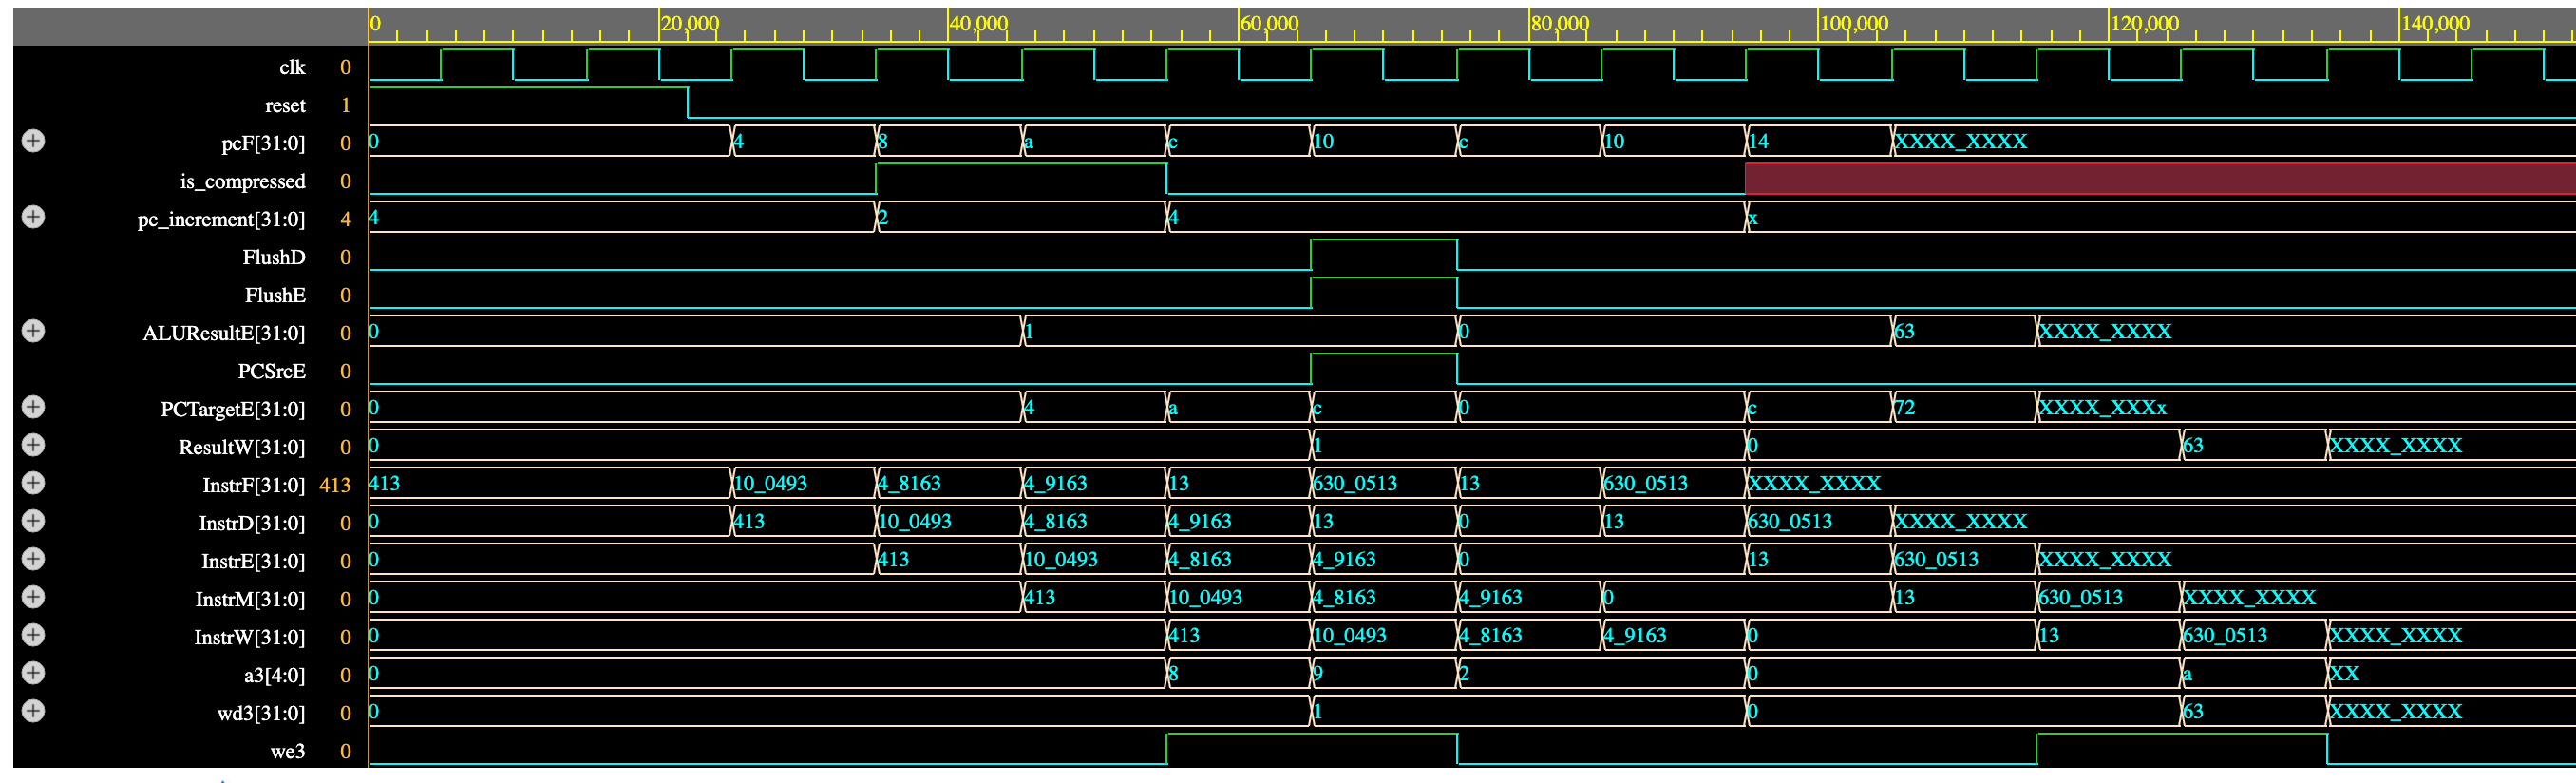
\includegraphics[width=0.95\textwidth]{../Images/Entrega2/waves_rvc_branches/waves_rvc_branches.png}
\caption{Forma de onda general del test de saltos RVC, mostrando la ejecución secuencial de las instrucciones y la respuesta del pipeline.}
\label{fig:waves_rvc_branches_general}
\end{figure}

\begin{figure}[H]
\centering
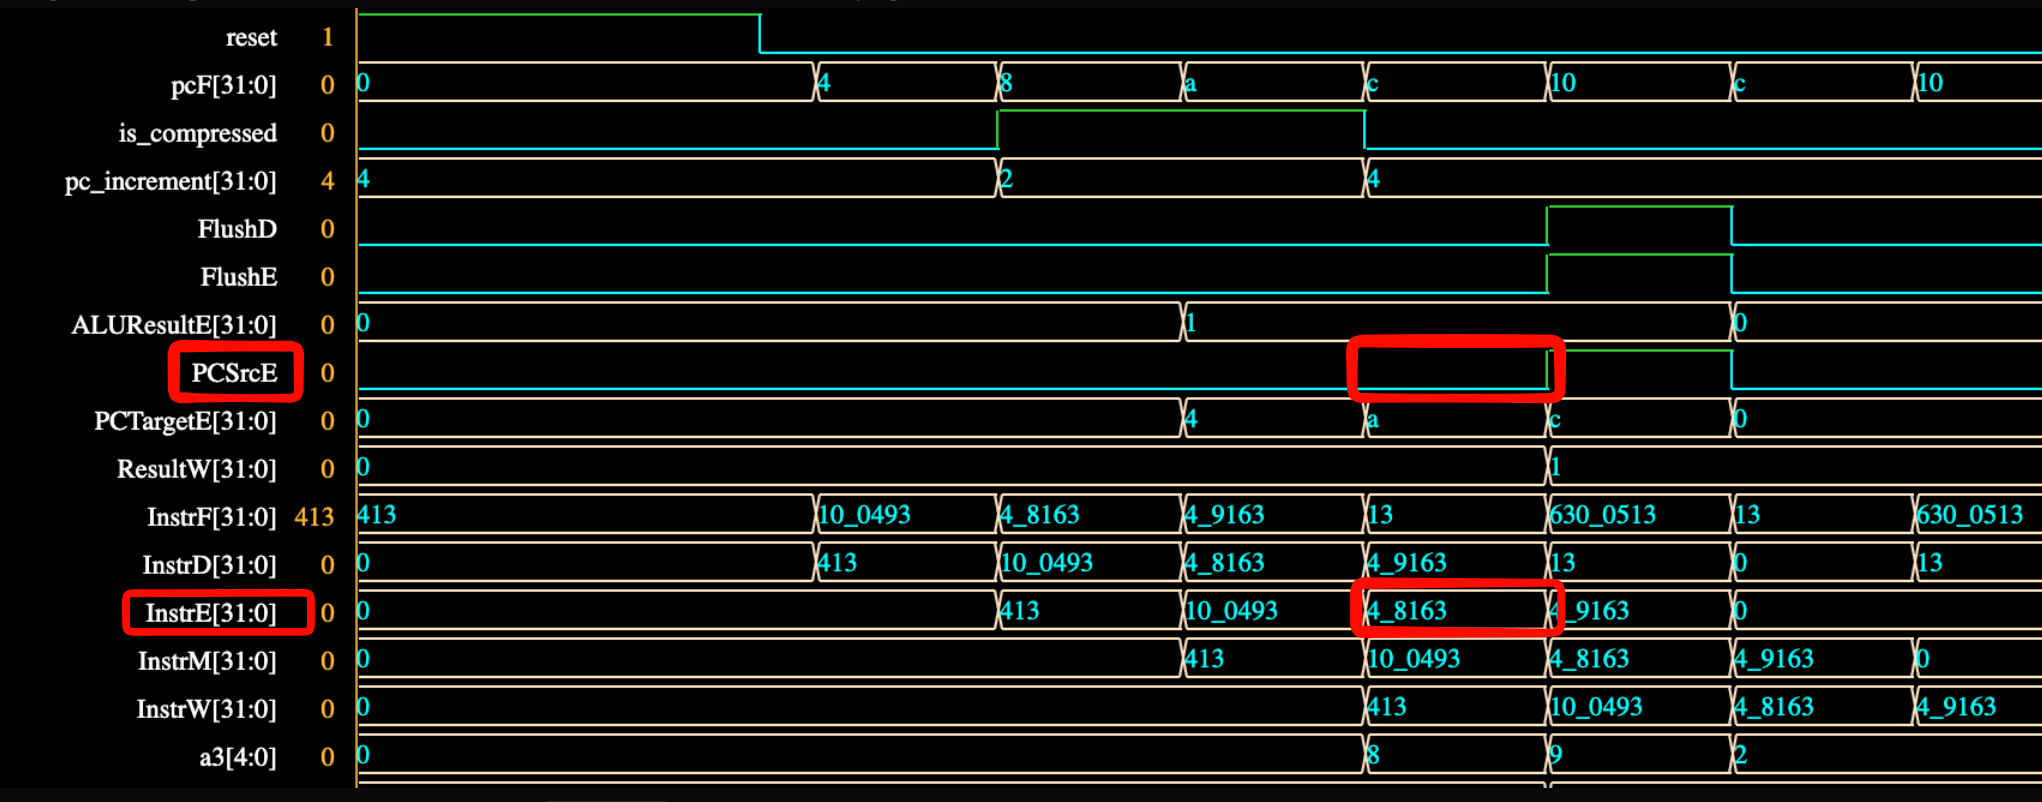
\includegraphics[width=0.95\textwidth]{../Images/Entrega2/waves_rvc_branches/waves_rvc_branches_e1.png.png}
\caption{Branch No Tomado}
\label{fig:waves_rvc_branches_e1}
\end{figure}

\textbf{Branch No Tomado:}
En la forma de onda de la Fig. \ref{fig:waves_rvc_branches_e1}:
Enmarca la señal \texttt{pcF} en \texttt{0x08}, y muestra que cuando esa instrucción esta en Execute (\texttt{InstrE}), la señal \texttt{PCSrcE} permanece en \texttt{0}.
\\
*Qué decir en tu informe:*
Aquí se evalúa la instrucción \texttt{c.beqz x9, 4}. Como el registro \texttt{x9 = 1} (no es cero), el salto condicional no se toma (\texttt{PCSrcE = 0}). El PC avanza linealmente de \texttt{0x08} a \texttt{0x0A}.

\begin{figure}[H]
\centering
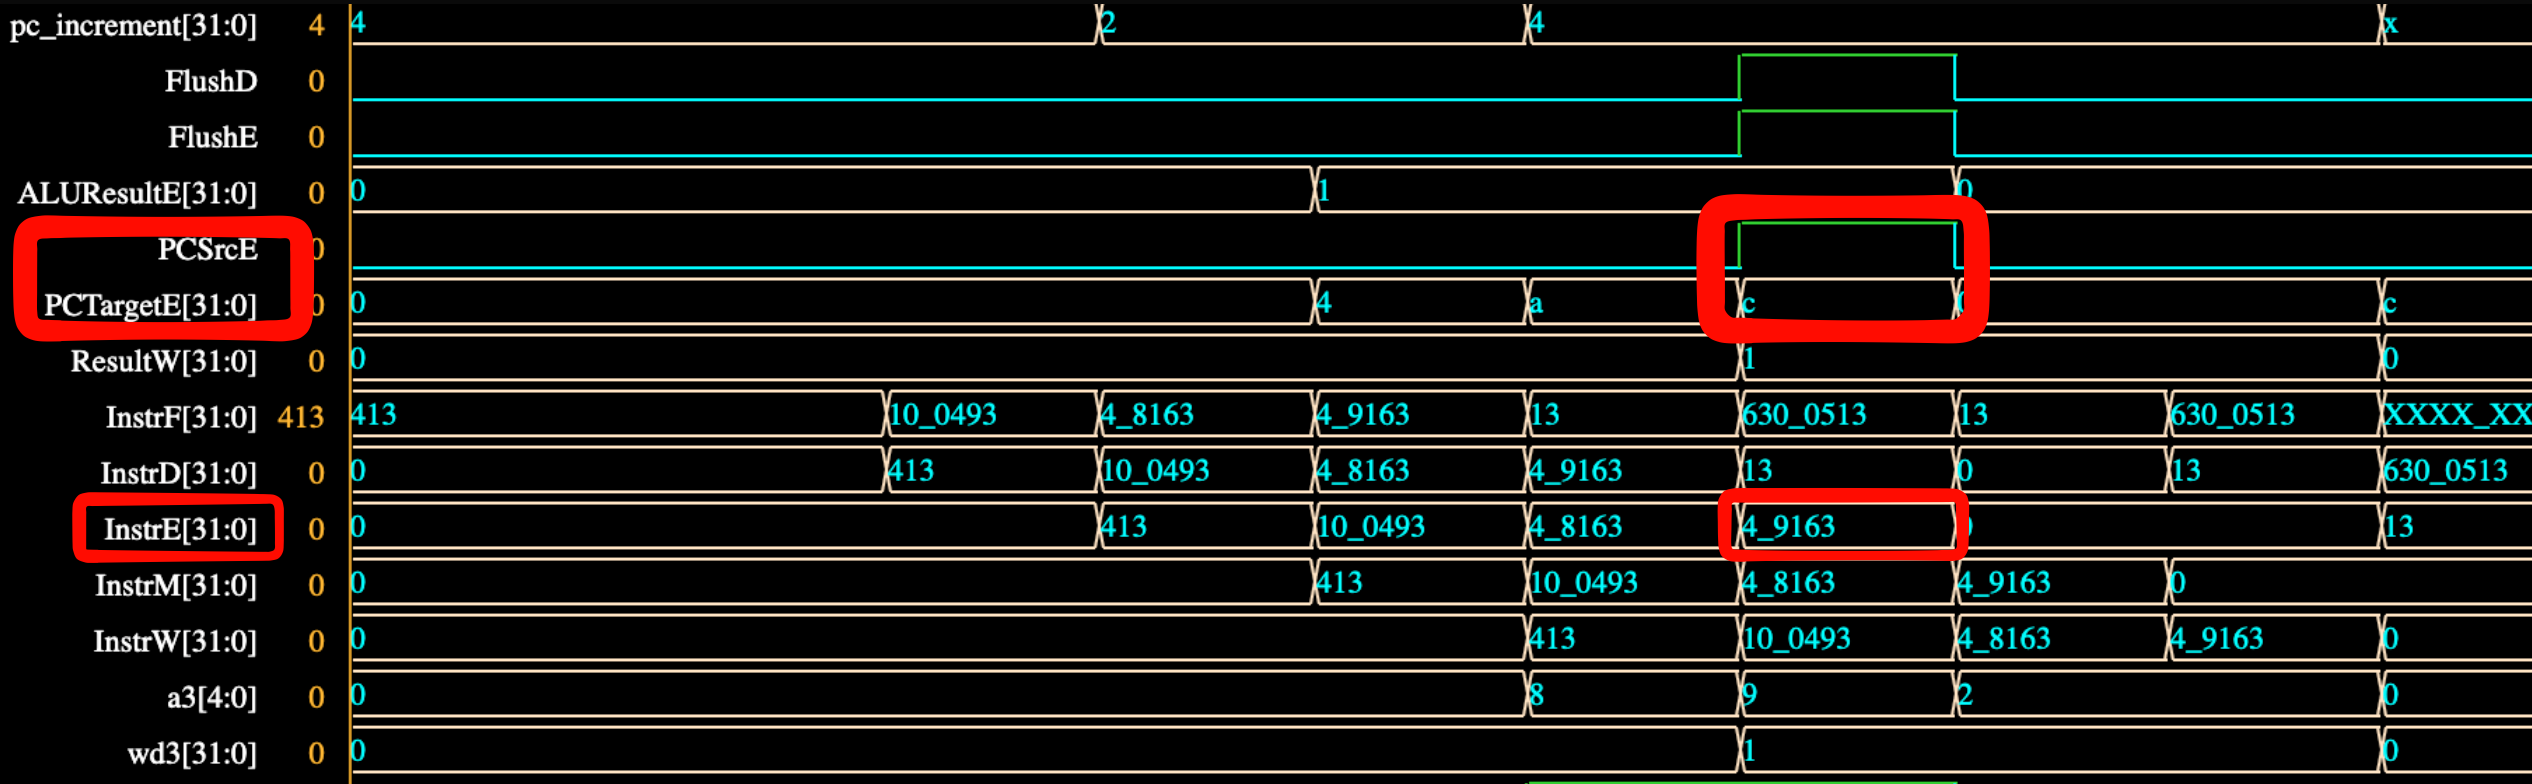
\includegraphics[width=0.95\textwidth]{../Images/Entrega2/waves_rvc_branches/waves_rvc_branches_e2.png.png}
\caption{Branch Tomado}
\label{fig:waves_rvc_branches_e2}
\end{figure}

\textbf{Branch Tomado:}
En la forma de onda de la Fig. \ref{fig:waves_rvc_branches_e2}:
Enmarca el ciclo donde la instrucción \texttt{c.bnez} llega a Execute (\texttt{InstrE = 00049163}). Senala que la bandera \texttt{PCSrcE} sube a \texttt{1}, la dirección destino \texttt{PCTargetE} marca \texttt{C} (hexadecimal) y en ese mismo instante el PC de Fetch (\texttt{pcF}) marca \texttt{10} (hexadecimal).
\\
*Qué decir en tu informe:*
Al evaluarse \texttt{c.bnez x9, 4} en Execute, dado que \texttt{x9 = 1 != 0}, la condición de salto se cumple. Se genera \texttt{PCSrcE = 1}, la dirección calculada de destino es \texttt{PCTargetE = 0x0C} (C en hex) y en ese instante el PC en Fetch marca \texttt{10} (hex) debido a la precarga secuencial.

\begin{figure}[H]
\centering
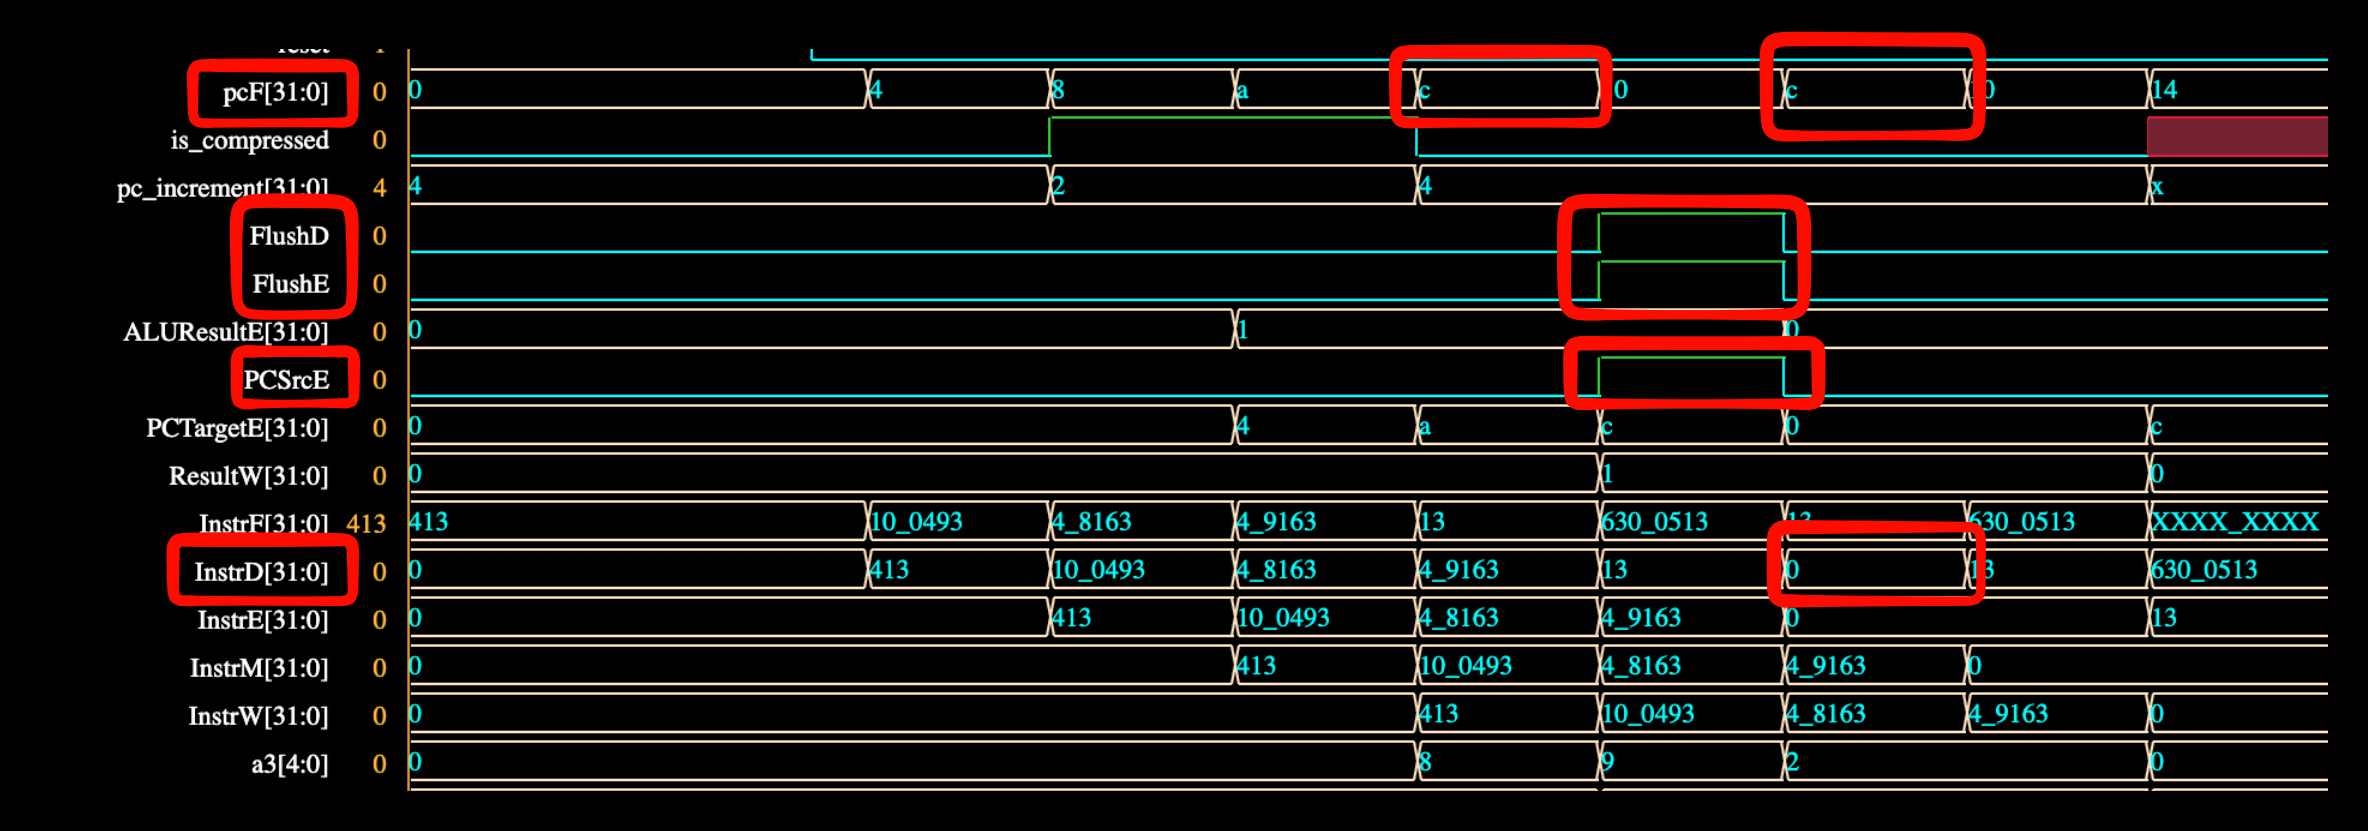
\includegraphics[width=0.95\textwidth]{../Images/Entrega2/waves_rvc_branches/waves_rvc_branches_e3.png}
\caption{Activacion de Burbujas}
\label{fig:waves_rvc_branches_e3}
\end{figure}

\textbf{Activacion de Burbujas:}
En la forma de onda de la Fig. \ref{fig:waves_rvc_branches_e3}:
Enmarca el ciclo donde \texttt{FlushD} y \texttt{FlushE} se ponen en \texttt{1} (ocurre al mismo tiempo que \texttt{PCSrcE = 1}). Enmarca también la señal \texttt{InstrD} en el ciclo siguiente, mostrando que el \texttt{nop} especulativo cargado en \texttt{0x0C} se limpia (se vuelve \texttt{0x00000000}), y el PC de Fetch (\texttt{pcF}) regresa a \texttt{C} (hexadecimal).
\\
*Qué decir en tu informe:*
Cuando el salto es tomado (\texttt{PCSrcE = 1}), las señales \texttt{FlushD} y \texttt{FlushE} de la Hazard Unit se activan en alto. Esto limpia de inmediato las etapas Decode y Execute, convirtiendo la instrucción especulativa de \texttt{0x0C} en un NOP para evitar que altere registros. En Fetch, el \texttt{pcF} se corrige y regresa a la dirección destino \texttt{0x0C}.

\begin{figure}[H]
\centering
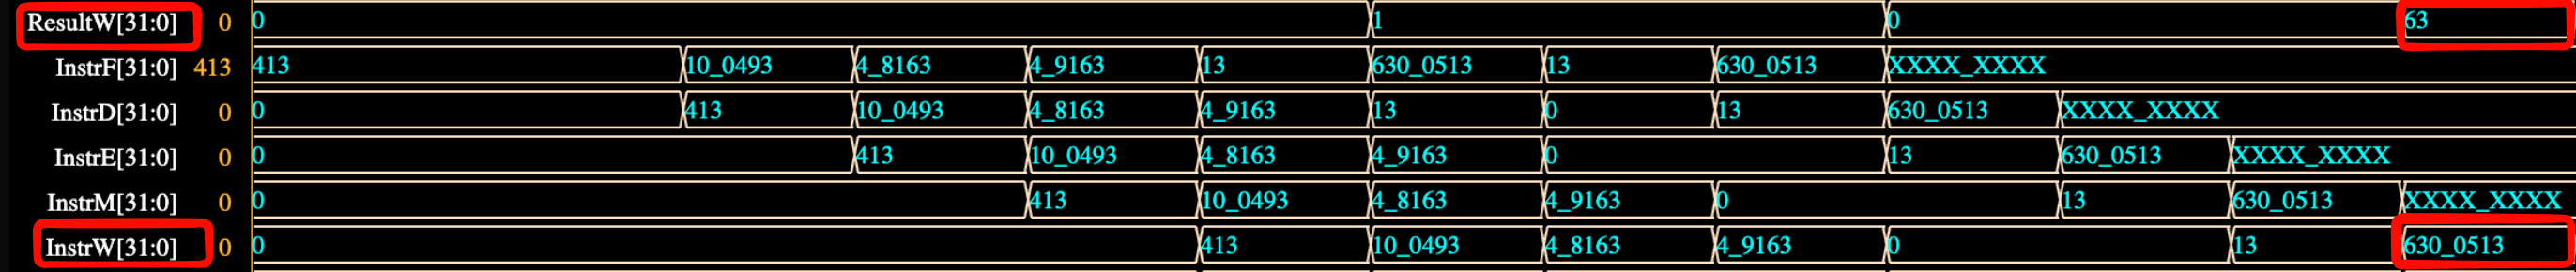
\includegraphics[width=0.95\textwidth]{../Images/Entrega2/waves_rvc_branches/waves_rvc_branches_e4.png}
\caption{Escritura del Registro Destino}
\label{fig:waves_rvc_branches_e4}
\end{figure}

\textbf{Escritura del Registro Destino:}
En la forma de onda de la Fig. \ref{fig:waves_rvc_branches_e4}:
Enmarca la señal \texttt{ResultW[31:0]} mostrando el valor \texttt{63} (hexadecimal de \texttt{99}), y al mismo tiempo enmarca la señal \texttt{InstrW[31:0]} mostrando el valor \texttt{06300513} (que representa a \texttt{addi x10, x0, 99}) en el ultimo ciclo.
\\
*Qué decir en tu informe:*
Se comprueba que la instrucción destino del salto (\texttt{addi x10, x0, 99}) se completa con éxito: en la etapa de Writeback (WB), la señal `InstrW` muestra `06300513` y `ResultW` escribe el valor correcto `63` (99 en decimal) en el banco de registros, validando el correcto funcionamiento del pipeline.

\subsubsection{Test RVC de Cobertura Completa (\texttt{test\_rvc\_remaining.mem})}
El test de cobertura completa tiene como finalidad validar las 14 instrucciones de la extension comprimida RVC especificadas en el proyecto que no fueron evaluadas en las pruebas anteriores. Esto garantiza el cumplimiento total de la tabla de instrucciones del diseño. El programa ejecuta la siguiente secuencia de instrucciones:

\begin{lstlisting}[style=pseudo, caption={Programa RVC Cobertura Completa: test\_rvc\_remaining.mem}]
0x00: c.addi sp, 16        // Inicializar Stack Pointer sp (x2) = 16
0x02: c.addi x8, 12        // x8 = 12
0x04: c.addi x9, 3         // x9 = 3
0x06: c.addi x10, 10       // x10 = 10
0x08: c.addi x12, 5        // x12 = 5
0x0A: c.addi x13, 8        // x13 = 8
0x0C: c.lui x11, 4         // x11 = 4 << 12 = 16384 (U-type)
0x0E: c.slli x8, 2         // x8 = x8 << 2 = 48
0x10: c.srli x9, 1         // x9 = x9 >> 1 = 1
0x12: c.srai x8, 3         // x8 = x8 >> 3 = 6
0x14: c.andi x10, 7        // x10 = x10 & 7 = 2
0x16: c.andi x9, 3         // x9 = x9 & 3 = 1
0x18: c.xor x10, x12       // x10 = x10 ^ x12 = 2 ^ 5 = 7
0x1A: c.or x10, x13        // x10 = x10 | x13 = 7 | 8 = 15
0x1C: c.and x10, x9        // x10 = x10 & x9 = 15 & 1 = 1
0x1E: c.add x11, x12       // x11 = x11 + x12 = 16384 + 5 = 16389
0x20: c.swsp x11, 4(sp)    // Guardar x11 en sp+4 = 20 (Store SP)
0x22: c.lwsp x14, 4(sp)    // Cargar x14 desde sp+4 = 20 (Load SP)
0x24: c.jal target_jal     // Salto y enlace (x1 = PC+2 = 0x26), salta a 0x38
0x26: c.nop                // NOP de retorno del jal
0x28: addi x15, x0, 60     // Cargar dirección del jalr (60 = 0x3C) en x15
0x2C: c.jalr x15           // Salto y enlace indirecto, ra = 0x2E, salta a 0x3C
0x2E: c.nop                // NOP de retorno del jalr
0x30: c.j end_loop         // Bucle infinito de parada
0x32: c.nop                // Relleno
0x34: c.nop                // Relleno
0x36: c.nop                // Relleno
0x38: c.jr ra              // Retorno de jal: salta a ra (0x26)
0x3A: c.nop                // Relleno
0x3C: c.jr ra              // Retorno de jalr: salta a ra (0x2E)
\end{lstlisting}

\renewcommand{\thefigure}{21.\arabic{figure}}
\renewcommand{\theHfigure}{21.\arabic{figure}}
\setcounter{figure}{0}

\begin{figure}[H]
\centering
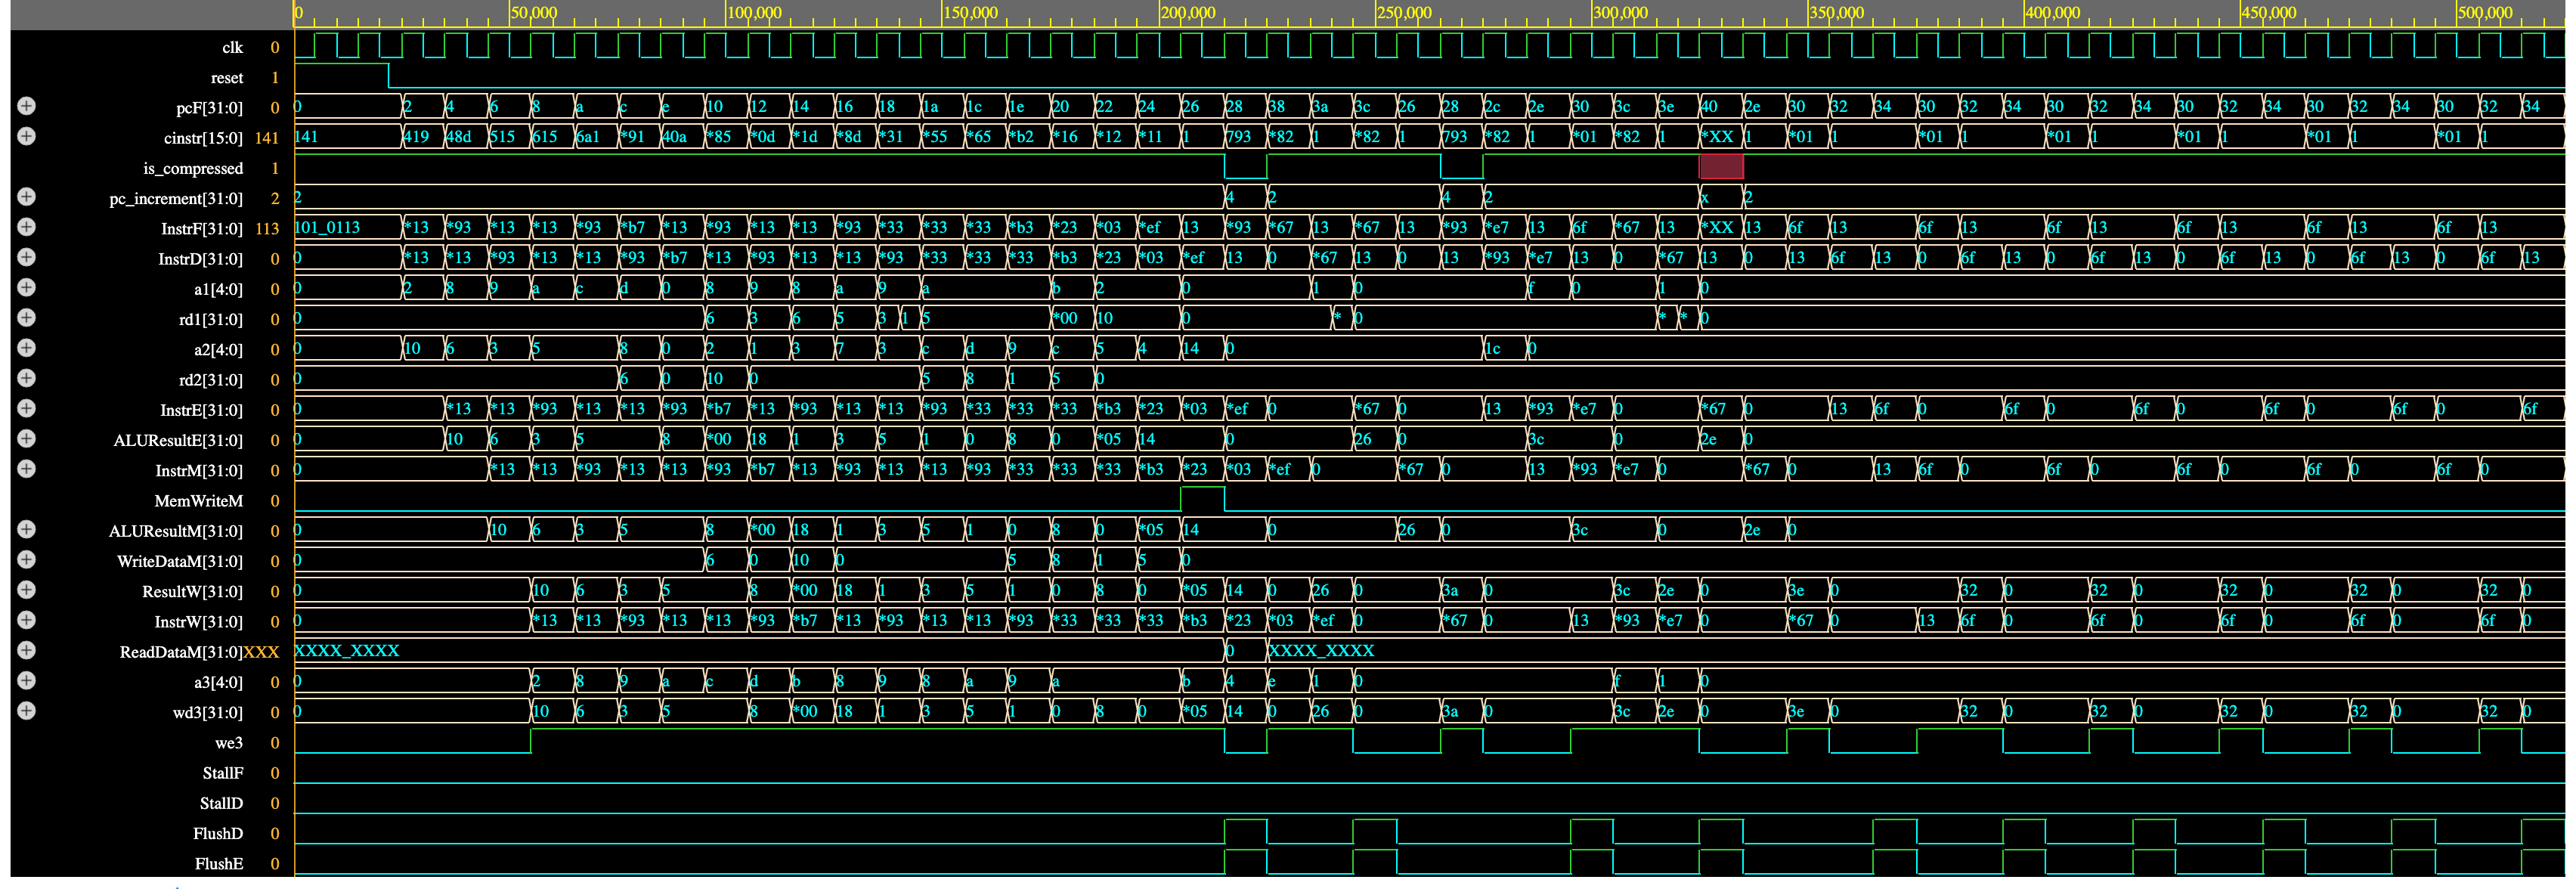
\includegraphics[width=0.95\textwidth]{../Images/Entrega2/waves_rvc_remaining/waves_rvc_remaining.png}
\caption{Forma de onda general del test de cobertura completa, validando las 14 instrucciones RVC restantes.}
\label{fig:waves_rvc_remaining_general}
\end{figure}

\textbf{Comprobacion y Analisis de los Aspectos Clave de la Simulación:}
A traves de la forma de onda de la Fig. \ref{fig:waves_rvc_remaining_general}, se puede analizar y comprobar la correcta ejecución e integracion de estas nuevas instrucciones en la microarquitectura segmentada, destacando tres aspectos fundamentales:

\begin{itemize}
  \item \textbf{Interaccion RVC con la Hazard Unit (Reenvio de Datos):} 
    El programa prueba directamente la resolución de dependencias tipo RAW entre instrucciones comprimidas. La instrucción \texttt{c.add x11, x12} (en PC \texttt{0x1E}) escribe en el registro destino \texttt{x11}, y la instrucción inmediatamente posterior, \texttt{c.swsp x11, 4(sp)} (en PC \texttt{0x20}), lee dicho registro como operando fuente. En el ciclo 18 de la simulación, mientras \texttt{c.swsp} esta en Execute (EX) y \texttt{c.add} esta en Memory (MEM), la Hazard Unit detecta la coincidencia de registros y activa la señal de reenvio \texttt{ForwardBE = 2'b10}. Esto inyecta de manera combinacional el valor correcto calculado por la ALU (\texttt{16389} o \texttt{0x00004005}) directamente en el bus de datos a escribir en memoria (\texttt{WriteDataM}) en el ciclo siguiente, sin insertar retardos ni burbujas en el pipeline.
    
  \item \textbf{Accesos a Memoria Relativos a Stack Pointer:} 
    Las instrucciones de pila se ejecutan con exito referenciando al registro \texttt{x2} (\texttt{sp}) cargado combinacionalmente:
    \begin{itemize}
      \item En la etapa MEM de \texttt{c.swsp} (ciclo 19), la señal \texttt{MemWriteM} se activa en alto (\texttt{1}) y se escribe el valor \texttt{16389} en la dirección de memoria calculada \texttt{ALUResultM = 20} (dirección base del \texttt{sp} en $16$ más el desplazamiento de $4$ bytes).
      \item En la etapa MEM de la instrucción consecutiva \texttt{c.lwsp x14, 4(sp)} (ciclo 20), la señal de control \texttt{MemWriteM} se desactiva a bajo (\texttt{0}) para realizar la lectura de la dirección \texttt{ALUResultM = 20}. La memoria RAM entrega el dato leido de 32 bits \texttt{0x00004005} (16389 decimal), el cual en la etapa de Writeback (WB) es escrito exitosamente en el registro destino \texttt{x14} a traves de los puertos de escritura del banco de registros (\texttt{we3 = 1}, \texttt{a3 = 14}, \texttt{wd3 = 0x4005}).
    \end{itemize}

  \item \textbf{Control de Flujo de Saltos Comprimidos y Enlace (Link):}
    \begin{itemize}
      \item \textbf{Salto y Enlace Relativo (\texttt{c.jal}):} Al evaluarse \texttt{c.jal target\_jal} (PC \texttt{0x24}) en la etapa Execute (ciclo 21), la ALU calcula el destino relativo \texttt{PCTargetE = 0x38}. La señal de control \texttt{PCSrcE} sube a \texttt{1}, corrigiendo el PC. Simultaneamente, la Hazard Unit activa \texttt{FlushD = 1} y \texttt{FlushE = 1} para vaciar la instrucción especulativa en Decode (el \texttt{c.nop} en \texttt{0x26}), insertando la burbuja. El registro de enlace \texttt{ra} (\texttt{x1}) se actualiza en Writeback con la dirección de retorno correcta \texttt{0x26} (correspondiente a \texttt{PC + 2}, validando que el hardware reconoce el ancho comprimido de la instrucción).
      \item \textbf{Retorno Indirecto (\texttt{c.jr ra}):} En la dirección \texttt{0x38}, la instrucción \texttt{c.jr ra} lee el registro de retorno \texttt{ra = 0x26} a traves del puerto \texttt{rd1} y salta de vuelta al pipeline secuencial.
      \item \textbf{Salto Indirecto con Enlace (\texttt{c.jalr}):} Se carga la dirección absoluta de \texttt{target\_jalr} (\texttt{60} o \texttt{0x3C}) en el registro \texttt{x15}. Al ejecutarse \texttt{c.jalr x15} en PC \texttt{0x2C}, la CPU salta a \texttt{0x3C} y almacena en el registro de enlace \texttt{ra} la dirección de retorno corregida \texttt{0x2E} (\texttt{PC + 2}). Finalmente, otra instrucción \texttt{c.jr ra} en \texttt{0x3C} retorna la ejecución a la dirección de parada del bucle infinito en \texttt{0x30}.
    \end{itemize}
\end{itemize}
De esta forma, se demuestra que todas las extensiones de control, descompresión y operaciones de datos de RVC interactuan de manera transparente con los mecanismos de riesgos del procesador segmentado, logrando una cobertura del 100\% de la ISA especificada y completando la verificacion exhaustiva.

\subsection{Analisis de Performance y Justificacion de la Extension RVC}
La incorporación de la extension RVC representa un compromiso de diseño (trade-off) entre el area de silicio, el consumo de potencia, la frecuencia de reloj y el tamaño del binario. A continuación se detallan los resultados del analisis de performance y las directrices arquitectonicas de uso.

\subsubsection{Analisis de Ciclos de Reloj (Timing Analysis)}
Una de las mayores ventajas de nuestra estrategia de diseño (descompresión combinacional en la etapa de Fetch) es la \textbf{ausencia de penalización en ciclos de reloj}. 
\begin{itemize}
    \item Debido a que la expansion de 16 a 32 bits se realiza en tiempo cero (combinacionalmente antes de registrar la instrucción en el buffer \texttt{IF/ID}), cada instrucción comprimida fluye a traves de las 5 etapas del pipeline exactamente de la misma forma que una instrucción RV32I.
    \item En la ejecución de la prueba básica (\texttt{test\_rvc\_basic.mem}), el programa RVC consta de 6 instrucciones efectivas (incluyendo un salto incondicional). Al igual que su equivalente en RV32I, el procesador requiere exactamente 12 ciclos de reloj para completar la ejecución de las 6 instrucciones, confirmando que la descompresión no anade burbujas ni latencia adicional al pipeline de datos.
    \item El único impacto de tiempo se da en el retardo de propagacion (critical path) de la etapa Fetch. La adicion del descompresor RVC (multiplexores combinacionales) y el multiplexor de alineacion (alignmux) introduce un retardo en el camino de lectura de instrucciones. Si bien en este procesador el critical path sigue estando dominado por la ALU (etapa Execute) o los retardos de memoria, en diseños a muy altas frecuencias esto podria reducir levemente la frecuencia maxima de reloj ($f_{max}$).
\end{itemize}

\subsubsection{Reducción de Tamaño de Código (Code Density)}
Para el programa básico evaluado, se realiza la comparación de consumo de bytes en memoria de instrucciones:
\begin{table}[H]
\centering
\begin{tabular}{l|c|c|c}
\toprule
\textbf{Instrucción} & \textbf{Ancho RV32I} & \textbf{Ancho RVC} & \textbf{Ahorro en Memoria} \\
\midrule
1. Inicializar x8 & 4 bytes (\texttt{addi}) & 2 bytes (\texttt{c.addi}) & 50\% \\
2. Inicializar x9 & 4 bytes (\texttt{addi}) & 2 bytes (\texttt{c.addi}) & 50\% \\
3. Suma x10 = x8 + x9 & 4 bytes (\texttt{add}) & 4 bytes (\texttt{add}) & 0\% \\
4. Resta x8 = x8 - x9 & 4 bytes (\texttt{sub}) & 2 bytes (\texttt{c.sub}) & 50\% \\
5. Salto incondicional & 4 bytes (\texttt{jal}) & 2 bytes (\texttt{c.j}) & 50\% \\
6. NOP & 4 bytes (\texttt{nop}) & 4 bytes (\texttt{nop}) & 0\% \\
7. Escritura final x11 & 4 bytes (\texttt{addi}) & 4 bytes (\texttt{addi}) & 0\% \\
\midrule
\textbf{Total Programa} & \textbf{28 bytes} & \textbf{20 bytes} & \textbf{28.5\%} \\
\bottomrule
\end{tabular}
\caption{Comparativa del tamaño de código en memoria entre la implementación RV32I y RVC para el test básico.}
\label{tab:ahorro_memoria}
\end{table}

Este resultado del 28.5\% de ahorro en memoria de instrucciones demuestra empíricamente que RVC cumple con el objetivo de diseño teorico (tipicamente entre 25\% y 30\% de reducción), permitiendo almacenar programas más grandes en memorias fisicamente más pequenas.

\subsubsection{Guia de Uso: Cuando usar RVC y cuando no}
El empleo de la extension RVC se justifica bajo ciertos escenarios de diseño de hardware:
\begin{itemize}
    \item \textbf{Por que y cuando usar RVC (Ventajas):}
    \begin{enumerate}
        \item \textbf{Limitacion de Memoria (Sistemas Embebidos):} En microcontroladores o dispositivos IoT con memoria flash interna muy reducida (ej. 32 KB a 256 KB), el ahorro de un 30\% del espacio permite añadir mayor funcionalidad al firmware sin aumentar el costo del chip.
        \item \textbf{Mejora en la Cache de Instrucciones (I-Cache):} Al comprimir el código, caben más instrucciones en una misma línea de cache, lo que reduce la tasa de fallos de cache (cache misses) y mejora el rendimiento general del procesador ante accesos lentos a la memoria principal.
        \item \textbf{Reducción de Consumo de Energia:} Dado que se transfieren menos bits por los buses de memoria externa en cada fetch de instrucción, el consumo de energia dinamica disminuye significativamente.
    \end{enumerate}
    
    \item \textbf{Cuando NO usar RVC (Limitaciones):}
    \begin{enumerate}
        \item \textbf{Procesadores Superescalares de Muy Alto Rendimiento:} En procesadores que decodifican 4 o más instrucciones en paralelo por ciclo, la descompresión RVC paralela anade una complejidad circuital y un area de silicio prohibitivas, limitando la frecuencia de reloj.
        \item \textbf{Buses de Memoria Anchos no Optimizados:} Si el procesador cuenta con un bus de datos extremadamente ancho hacia la memoria y la capacidad de almacenamiento no es una restricción de diseño (ej. computadoras de escritorio o servidores), el hardware de descompresión combinacional introduce un retardo innecesario en la etapa de Fetch.
    \end{enumerate}
\end{itemize}

\subsection{Analisis de Modos de Fallo de la Extension RVC}
Con el fin de validar la robustez de la extension RVC y demostrar de manera practica que ocurre ante fallos en los nuevos componentes de Fetch, se realizo una simulación mediante inyeccion de fallos. En particular, se evaluo el \textbf{Fallo en el Incremento Dinamico (Incremento rigido a +4)}.

Este fallo se inyecto forzando la señal \texttt{pc\_increment = 32'd4} de manera estatica en el módulo \texttt{fetch.v}, ignorando el valor de la bandera de descompresión \texttt{is\_compressed}. 

A continuación se presenta la comparación ciclo a ciclo de las trazas de simulación (wave-tables) para el flujo correcto y el flujo con fallo utilizando el test RVC básico (\texttt{test\_rvc\_basic.mem}):

\begin{table}[H]
\centering
\small
\resizebox{\textwidth}{!}{%
\begin{tabular}{c|l|l|l|l|l}
\toprule
\textbf{Ciclo} & \textbf{Etapa IF (PC)} & \textbf{Etapa ID (Instr)} & \textbf{Etapa EX (Instr)} & \textbf{ALUResultE} & \textbf{Efecto / Estado} \\
\midrule
\multicolumn{6}{c}{\textbf{Ejecución Correcta (Incremento Dinamico Activo)}} \\
\midrule
0 & PC = 0x00 & Instr = -- & Instr = -- & -- & Fetch c.addi x8, 5 \\
1 & PC = 0x02 & Instr = c.addi x8, 5 & Instr = -- & -- & Fetch c.addi x9, 10 (+2 bytes) \\
2 & PC = 0x04 & Instr = c.addi x9, 10 & Instr = c.addi x8, 5 & ALUResult = 5 & Fetch add x10, x8, x9 \\
3 & PC = 0x08 & Instr = add x10, x8, x9 & Instr = c.addi x9, 10 & ALUResult = 10 & x8 = 5 (WB). Fetch c.sub (+4 bytes) \\
4 & PC = 0x0A & Instr = c.sub x8, x9 & Instr = add x10, x8, x9 & ALUResult = 15 & x9 = 10 (WB). x10 = 15 (Correcto) \\
\midrule
\multicolumn{6}{c}{\textbf{Ejecución con Fallo (Incremento Rigido a +4)}} \\
\midrule
0 & PC = 0x00 & Instr = -- & Instr = -- & -- & Fetch c.addi x8, 5 \\
1 & PC = 0x04 & Instr = c.addi x8, 5 & Instr = -- & -- & Fetch add x10, x8, x9 (¡Salta 0x02!) \\
2 & PC = 0x08 & Instr = add x10, x8, x9 & Instr = c.addi x8, 5 & ALUResult = 5 & Fetch c.sub. ¡x9 sigue en 0! \\
3 & PC = 0x0C & Instr = c.sub x8, x9 & Instr = add x10, x8, x9 & ALUResult = 5 & x8 = 5 (WB). x10 = 5 (ERRONEO) \\
\bottomrule
\end{tabular}%
}
\caption{Comparativa de la traza de ejecución (wave-table) entre la ejecución correcta de RVC y la ejecución con fallo de incremento rigido a +4.}
\label{tab:comparativa_fallo}
\end{table}

\subsubsection{Analisis de Consecuencias del Fallo}
Al observar la comparación de trazas en la Tabla \ref{tab:comparativa_fallo} y analizando las señales del puerto de escritura del banco de registros (donde \texttt{a3} es la dirección del registro, \texttt{wd3} es el dato a escribir y \texttt{we3} es la señal de habilitacion de escritura), se concluyen las siguientes consecuencias graves:
\begin{itemize}
    \item \textbf{Omision de Instrucciones (Omission Hazard):} En la ejecución con fallo, el PC avanza de \texttt{0x00} directamente a \texttt{0x04}. La instrucción comprimida \texttt{c.addi x9, 10} ubicada en la dirección \texttt{0x02} jamas es cargada por el procesador, perdiéndose instrucciones críticas del programa.
    \item \textbf{Ausencia de Escritura del Registro Destino (\texttt{we3}/\texttt{a3}):} Dado que la instrucción de \texttt{0x02} fue omitida, el registro \texttt{x9} nunca recibe su valor de \texttt{10}. En la traza con fallo se observa que la habilitacion \texttt{we3} nunca se activa con la dirección \texttt{a3 = 9} (x9), de modo que dicho registro permanece en su estado inicial de cero (\texttt{0}).
    \item \textbf{Propagacion de Datos Corruptos (\texttt{wd3}):} Cuando la instrucción \texttt{add x10, x8, x9} (en \texttt{0x04}) llega a Execute, realiza la suma utilizando el valor no inicializado de \texttt{x9 = 0}. En consecuencia, cuando llega a Writeback, la dirección de escritura \texttt{a3} selecciona el registro \texttt{10} (\texttt{x10}) pero el dato escrito \texttt{wd3} toma el valor corrupto de \texttt{5} en lugar de \texttt{15}.
    \item \textbf{Desalineacion y Saltos Invalidos:} Si el código continuara y tratara de ejecutar un salto relativo comprimido, los desplazamientos calculados en base a un PC incorrecto harian que la CPU salte a direcciones desalineadas, decodificando datos basura y provocando una excepcion de instrucción ilegal.
\end{itemize}

\subsubsection{Comparativa Visual de Oscilogramas (Correcto vs. Fallo)}
Para corroborar empíricamente las consecuencias del fallo de incremento rigido a +4, se presentan a continuación las capturas de pantalla obtenidas directamente de la simulación en GTKWave. Cada comparativa consta de la traza funcional (izquierda) y la traza con fallo inyectado (derecha).

\renewcommand{\thefigure}{22.\arabic{figure}}
\renewcommand{\theHfigure}{22.\arabic{figure}}
\setcounter{figure}{0}

En la Fig. \ref{fig:good_e1} y \ref{fig:bad_e1} se compara el avance del PC de Fetch (\texttt{pcF}) y la señal del incrementador (\texttt{pc\_increment}). 

\begin{figure}[H]
  \centering
  \begin{minipage}{0.48\textwidth}
    \centering
    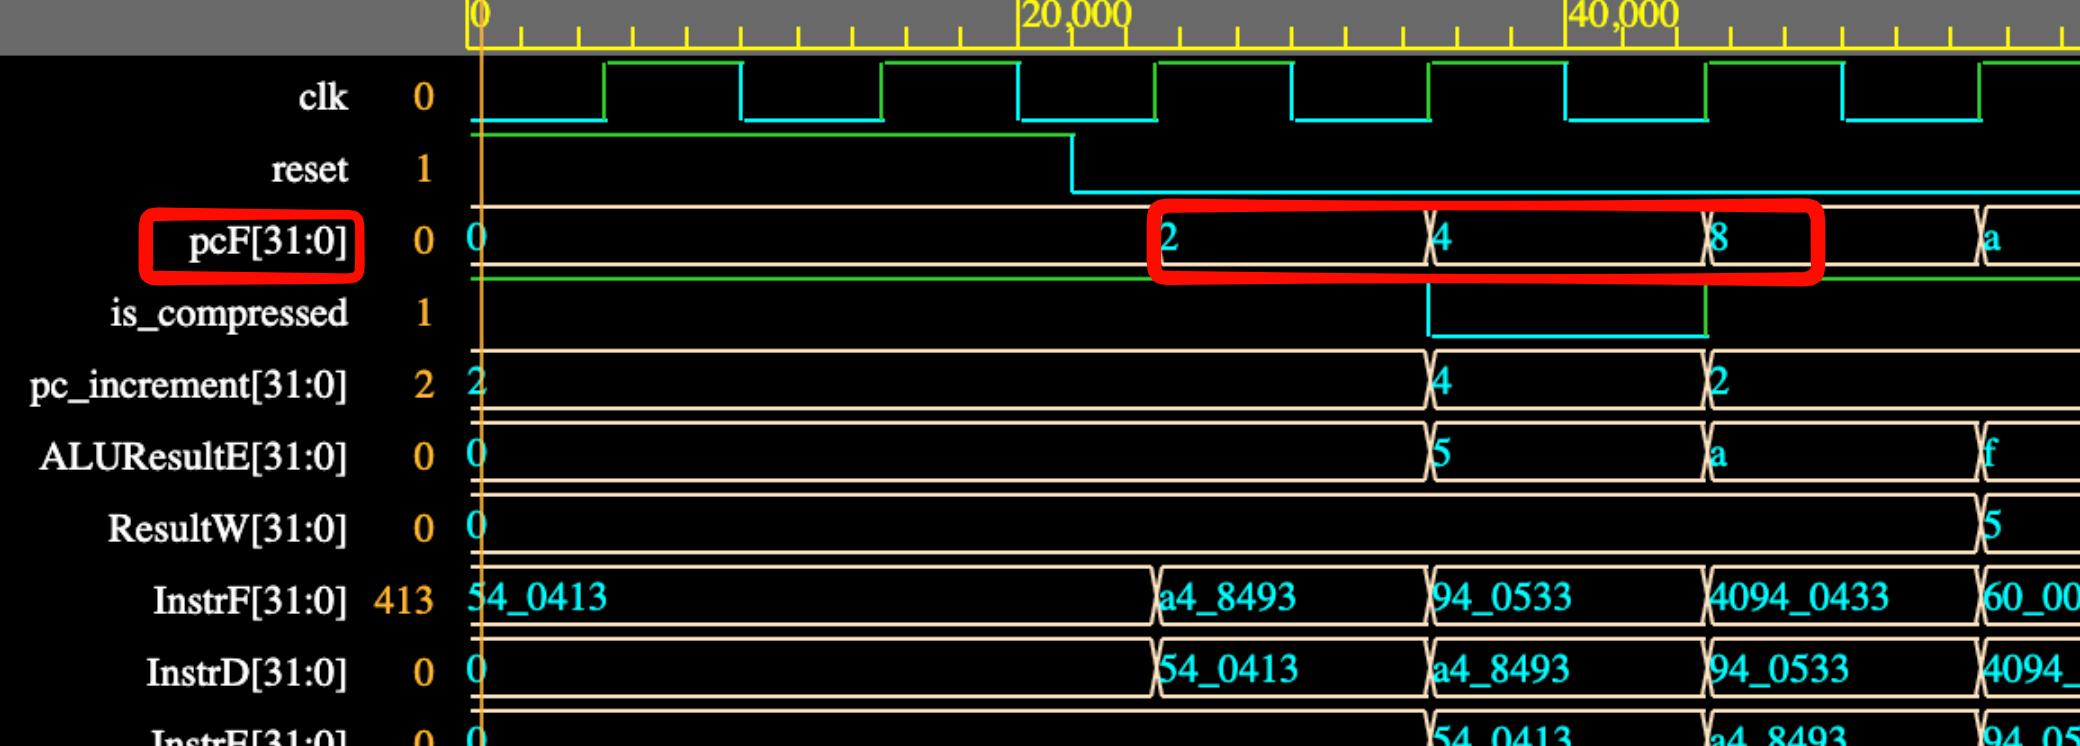
\includegraphics[width=\textwidth]{../Images/Entrega2/comparative/good_e1.png}
    \caption{Ejecución Correcta: El PC avanza de 0 a 2 y luego a 4 de manera dinamica.}
    \label{fig:good_e1}
  \end{minipage}
  \hfill
  \begin{minipage}{0.48\textwidth}
    \centering
    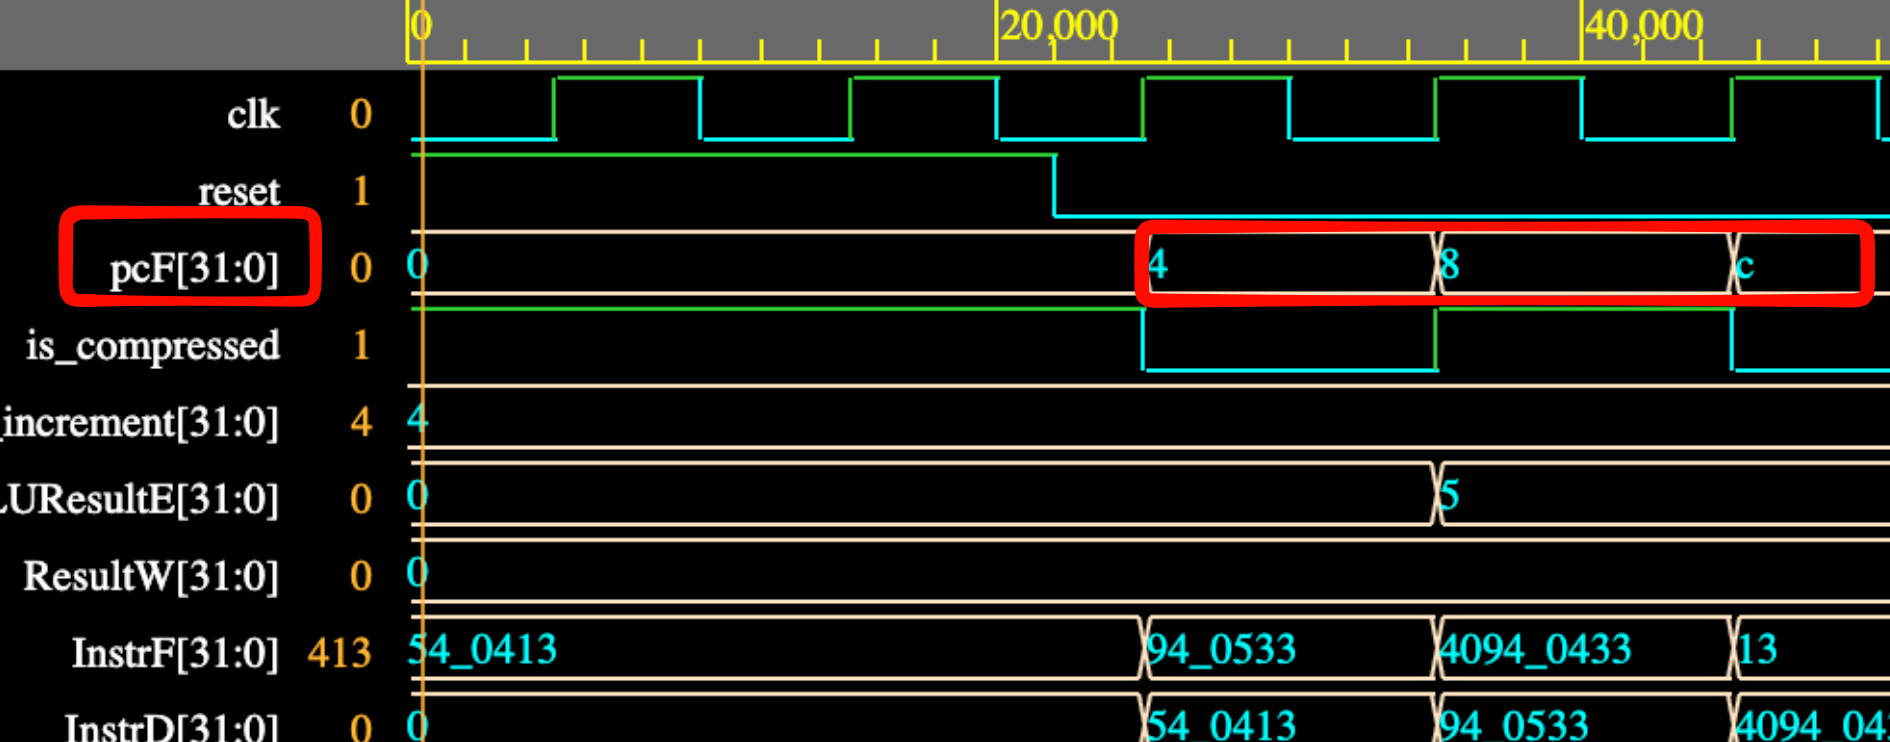
\includegraphics[width=\textwidth]{../Images/Entrega2/comparative/bad_e1.png}
    \caption{Ejecución con Fallo: El PC salta de 0 directamente a 4, omitiendo la dirección 0x02.}
    \label{fig:bad_e1}
  \end{minipage}
\end{figure}

Como se observa en la Fig. \ref{fig:good_e1}, la señal \texttt{pc\_increment} se activa en \texttt{2} en los ciclos correspondientes a instrucciones de 16 bits (\texttt{c.addi}), permitiendo que la ejecución secuencial sea perfecta. Por el contrario, en la Fig. \ref{fig:bad_e1}, la señal \texttt{pc\_increment} se mantiene rigidamente en \texttt{4}, lo que provoca la omision de la instrucción comprimida en \texttt{0x02}.

La Fig. \ref{fig:good_e3} y \ref{fig:bad_e3} muestra la instrucción decodificada en la etapa Decode (\texttt{InstrD}).

\begin{figure}[H]
  \centering
  \begin{minipage}{0.48\textwidth}
    \centering
    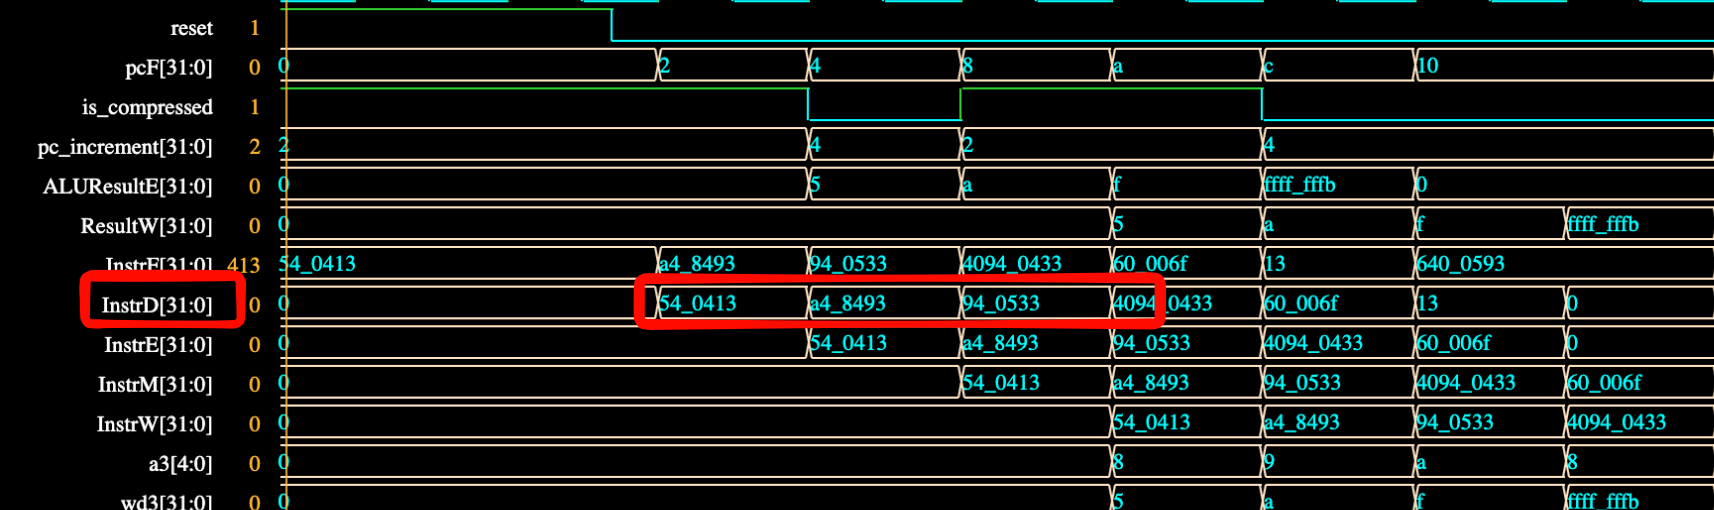
\includegraphics[width=\textwidth]{../Images/Entrega2/comparative/good_e3.png}
    \caption{Ejecución Correcta: Decodificacion secuencial de las tres instrucciones.}
    \label{fig:good_e3}
  \end{minipage}
  \hfill
  \begin{minipage}{0.48\textwidth}
    \centering
    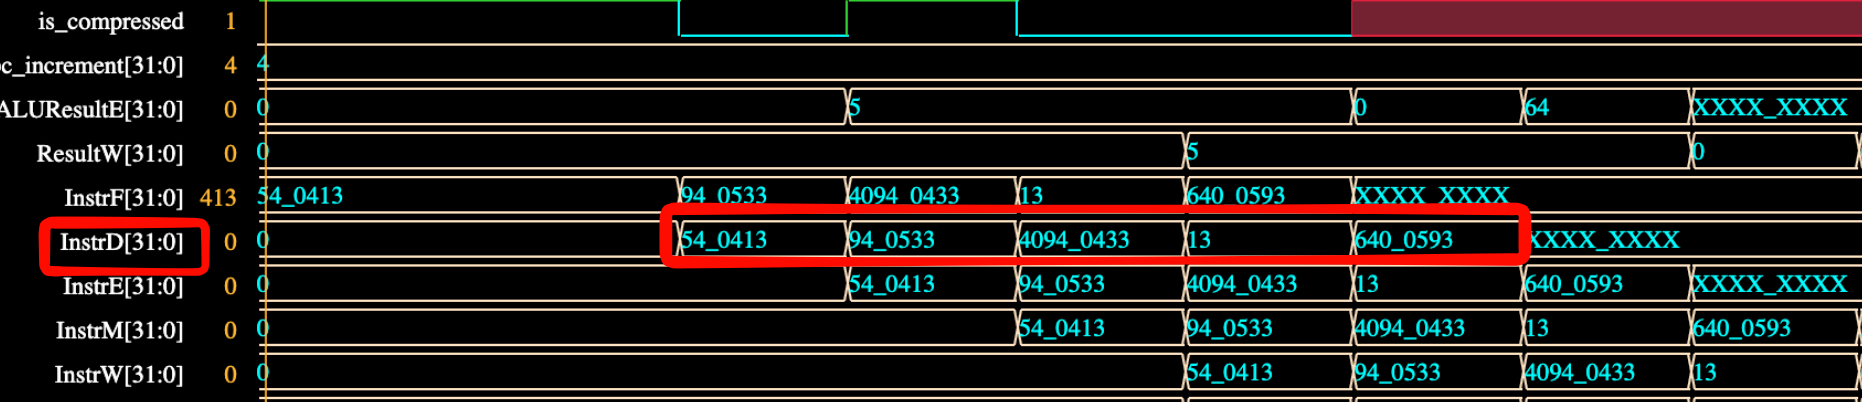
\includegraphics[width=\textwidth]{../Images/Entrega2/comparative/bad_e3.png}
    \caption{Ejecución con Fallo: La instrucción comprimida no aparece en Decode.}
    \label{fig:bad_e3}
  \end{minipage}
\end{figure}

En la ejecución correcta (Fig. \ref{fig:good_e3}), la etapa Decode recibe de manera secuencial la instrucción \texttt{c.addi x8, 5} (descomprimida como \texttt{0x00540413}), luego la instrucción \texttt{c.addi x9, 10} (descomprimida como \texttt{0x00a48493}), y por ultimo la instrucción \texttt{add x10, x8, x9} (\texttt{0x00940533}). En la ejecución con fallo (Fig. \ref{fig:bad_e3}), se pasa de la primera instrucción de suma inmediata directamente a la instrucción \texttt{add}, confirmando que la instrucción intermedia de \texttt{0x02} jamas entro en la etapa de decodificacion.

La Fig. \ref{fig:good_e2} y \ref{fig:bad_e2} muestra los puertos de escritura del banco de registros, analizando la habilitacion de escritura (\texttt{we3}), la dirección de escritura (\texttt{a3}) y el dato a escribir (\texttt{wd3}).

\begin{figure}[H]
  \centering
  \begin{minipage}{0.48\textwidth}
    \centering
    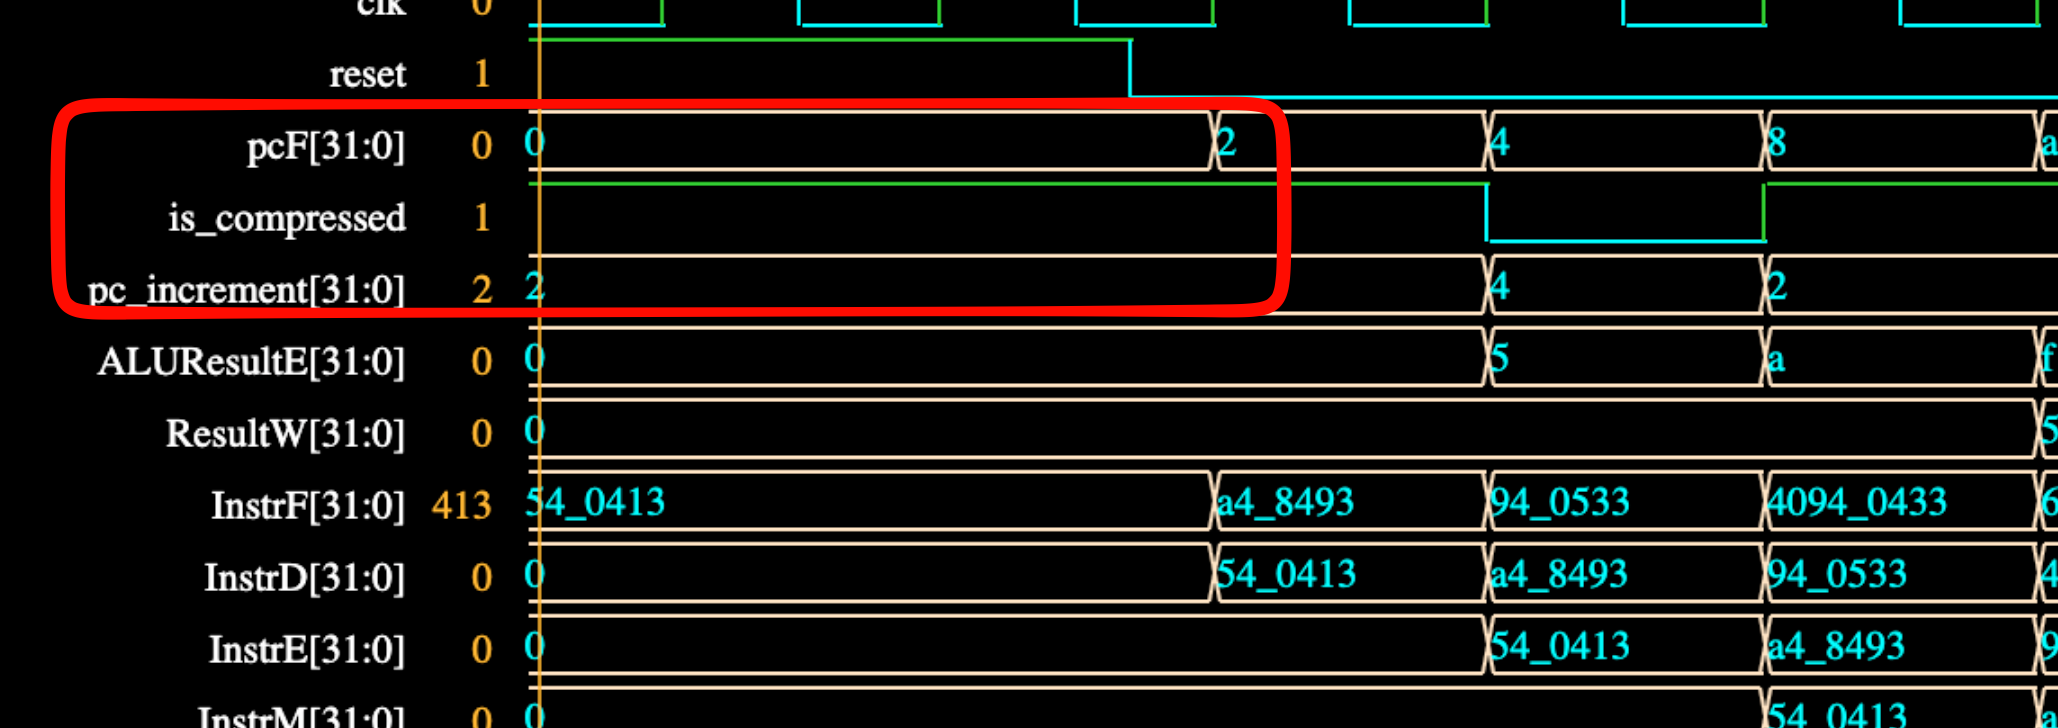
\includegraphics[width=\textwidth]{../Images/Entrega2/comparative/good_e2.png}
    \caption{Ejecución Correcta: Escritura exitosa de x8=5, x9=10 y x10=15.}
    \label{fig:good_e2}
  \end{minipage}
  \hfill
  \begin{minipage}{0.48\textwidth}
    \centering
    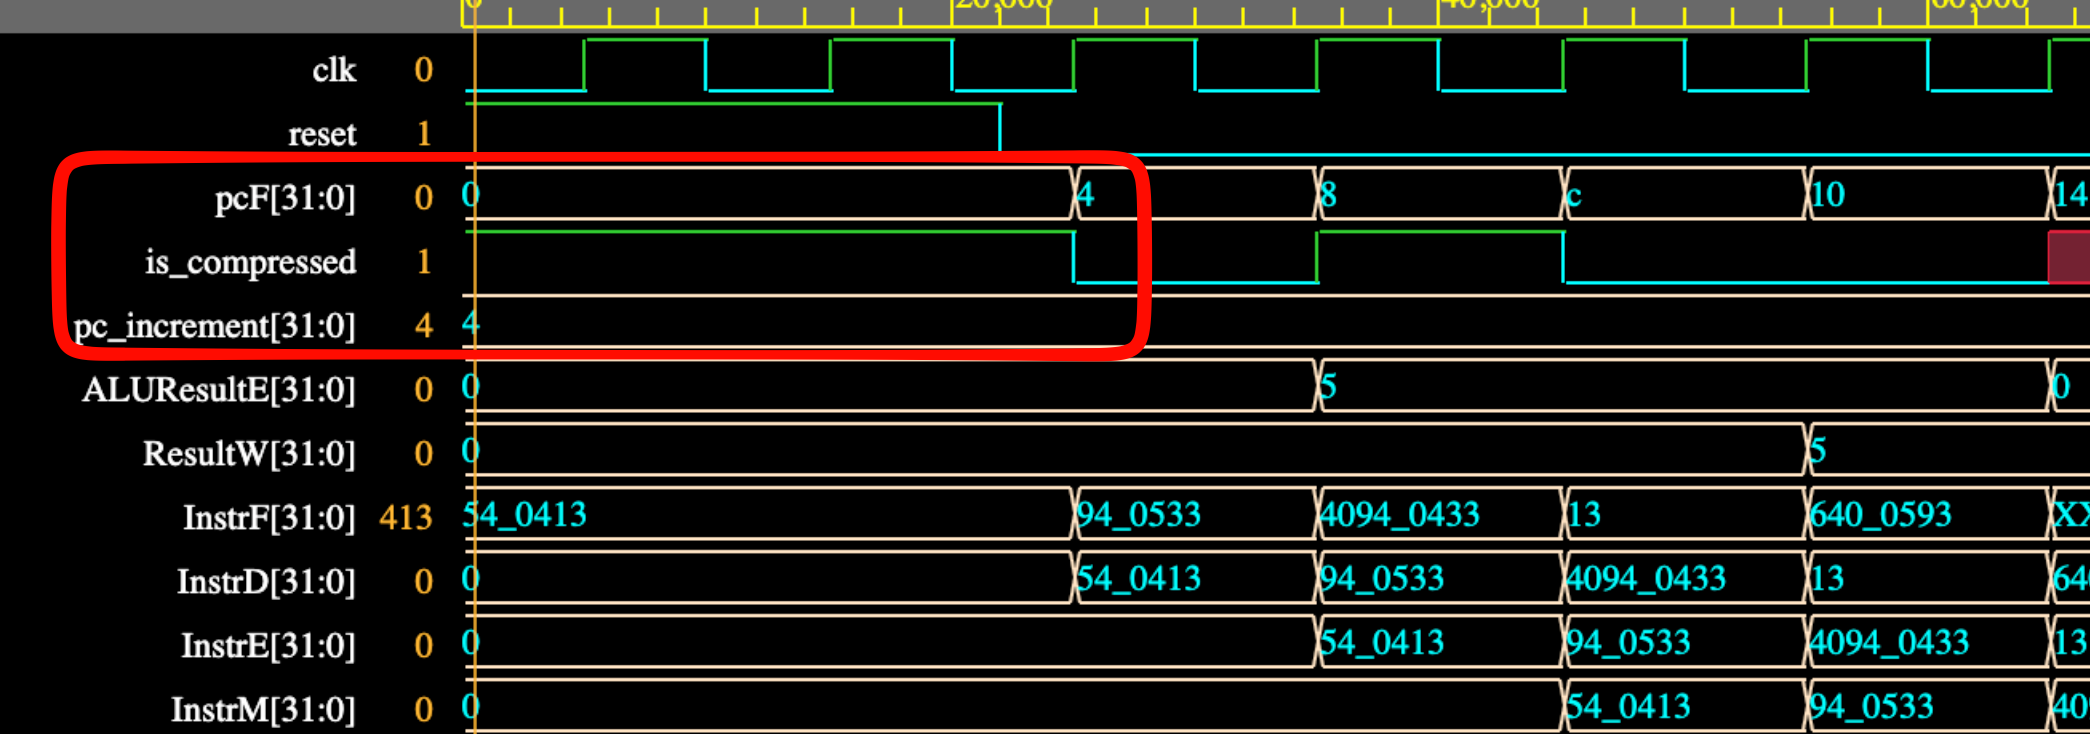
\includegraphics[width=\textwidth]{../Images/Entrega2/comparative/bad_e2.png}
    \caption{Ejecución con Fallo: Escritura ausente en x9 y suma corrupta en x10.}
    \label{fig:bad_e2}
  \end{minipage}
\end{figure}

En la Fig. \ref{fig:good_e2}, se observa la escritura secuencial correcta en la etapa de Writeback, culminando con la escritura de \texttt{15} (\texttt{0x0F}) en el registro destino \texttt{x10} (\texttt{a3 = 10}). Sin embargo, en la Fig. \ref{fig:bad_e2}, la escritura en el registro \texttt{x9} (\texttt{a3 = 9}) nunca se realiza debido a la omision de la instrucción, por lo que su valor permanece en \texttt{0}. Esto altera la ejecución de la instrucción \texttt{add x10, x8, x9}, la cual escribe en Writeback el valor erroneo de \texttt{5} (\texttt{0x05}) en el registro \texttt{x10}.

\renewcommand{\thefigure}{\arabic{figure}}
\renewcommand{\theHfigure}{\arabic{figure}}
\setcounter{figure}{21}

% ============================================================================
% SECCION 8: JERARQUIA DE ARCHIVOS
% ============================================================================
\section{Extension RVC - Segunda Parte (Entrega 3)}
La segunda parte de la extensión RVC (RISC-V Compressed) introduce soporte completo para operaciones de acceso a memoria, saltos condicionales e incondicionales (directos e indirectos), permitiendo que el procesador ejecute programas complejos con control de flujo y subrutinas codificados enteramente en 16 bits.

\subsection{Explicacion y Mapeo de las Instrucciones de la Segunda Parte}
Para dar cumplimiento a los requerimientos de la Entrega 3, a continuación se describe el formato de 16 bits, el comportamiento y el mapeo a la versión base de 32 bits (RV32I) de cada una de las 10 instrucciones correspondientes a la segunda parte:

\begin{enumerate}
    \item \textbf{c.lw (c.lw rd', imm(rs1')):}
    \begin{itemize}
        \item \textit{Funcionamiento:} Carga una palabra de 32 bits desde memoria en el registro restringido \texttt{rd'}. La dirección de memoria se forma sumando un inmediato positivo alineado a palabra (múltiplo de 4) al registro base \texttt{rs1'}.
        \item \textit{Mapeo RVC a RV32I:} Se expande a \texttt{lw rd, imm(rs1)}. Los registros destino \texttt{rd'} y fuente \texttt{rs1'} están restringidos al rango \texttt{x8-x15} (\texttt{cinstr[4:2]} y \texttt{cinstr[9:7]} respectivamente). El inmediato de 7 bits se reconstruye en bits no contiguos: \texttt{imm = {cinstr[5], cinstr[12:10], cinstr[6], 2'b00}}.
        \item \textit{Codigo Verilog:}
        \begin{lstlisting}[style=verilogstyle]
assign imm_lw_sw = {cinstr[5], cinstr[12:10], cinstr[6], 2'b00};
// En case (cinstr[15:13]) -> 3'b010:
outstr = {5'b0, imm_lw_sw, rdp_rs1p, 3'b010, rs2p, 7'b0000011};
        \end{lstlisting}
    \end{itemize}

    \item \textbf{c.sw (c.sw rs2', imm(rs1')):}
    \begin{itemize}
        \item \textit{Funcionamiento:} Almacena una palabra de 32 bits desde el registro restringido \texttt{rs2'} en memoria. La dirección de memoria se calcula sumando el inmediato positivo al registro base \texttt{rs1'}.
        \item \textit{Mapeo RVC a RV32I:} Se expande a \texttt{sw rs2, imm(rs1)}. Utiliza registros restringidos \texttt{x8-x15}. El inmediato de 7 bits se divide en dos campos para ajustarse al formato S-type de RV32I: \texttt{imm[11:5]} y \texttt{imm[4:0]}.
        \item \textit{Codigo Verilog:}
        \begin{lstlisting}[style=verilogstyle]
// En case (cinstr[15:13]) -> 3'b110:
outstr = {5'b0, imm_lw_sw[6:5], rs2p, rdp_rs1p, 3'b010, imm_lw_sw[4:0], 7'b0100011};
        \end{lstlisting}
    \end{itemize}

    \item \textbf{c.lwsp (c.lwsp rd, imm(sp)):}
    \begin{itemize}
        \item \textit{Funcionamiento:} Carga una palabra desde la pila en el registro completo \texttt{rd}. La dirección de memoria se forma sumando un inmediato positivo al registro Stack Pointer (\texttt{sp = x2}).
        \item \textit{Mapeo RVC a RV32I:} Se expande a \texttt{lw rd, imm(x2)}. Permite cualquier registro destino \texttt{rd} (\texttt{cinstr[11:7]}). El inmediato es de 8 bits scaled por 4: \texttt{imm = {cinstr[3:2], cinstr[12], cinstr[6:4], 2'b00}}.
        \item \textit{Codigo Verilog:}
        \begin{lstlisting}[style=verilogstyle]
assign imm_lwsp  = {cinstr[3:2], cinstr[12], cinstr[6:4], 2'b00};
// En case (cinstr[15:13]) -> 3'b010 (Cuadrante 2):
outstr = {4'b0, imm_lwsp, 5'd2, 3'b010, rd_rs1, 7'b0000011};
        \end{lstlisting}
    \end{itemize}

    \item \textbf{c.swsp (c.swsp rs2, imm(sp)):}
    \begin{itemize}
        \item \textit{Funcionamiento:} Guarda una palabra del registro completo \texttt{rs2} en la pila. La dirección se obtiene sumando un inmediato positivo al \texttt{sp}.
        \item \textit{Mapeo RVC a RV32I:} Se expande a \texttt{sw rs2, imm(x2)}. Permite guardar cualquier registro \texttt{rs2} (\texttt{cinstr[6:2]}). El inmediato de 8 bits se divide según el formato S-type de 32 bits.
        \item \textit{Codigo Verilog:}
        \begin{lstlisting}[style=verilogstyle]
assign imm_swsp  = {cinstr[8:7], cinstr[12:9], 2'b00};
// En case (cinstr[15:13]) -> 3'b110 (Cuadrante 2):
outstr = {4'b0, imm_swsp[7:5], rs2, 5'd2, 3'b010, imm_swsp[4:0], 7'b0100011};
        \end{lstlisting}
    \end{itemize}

    \item \textbf{c.beqz (c.beqz rs1', offset):}
    \begin{itemize}
        \item \textit{Funcionamiento:} Bifurcación condicional relativa al PC. Compara el contenido de \texttt{rs1'} con cero (\texttt{x0}); si son iguales, suma el inmediato con signo al PC.
        \item \textit{Mapeo RVC a RV32I:} Se expande a \texttt{beq rs1, x0, offset}. Utiliza el registro restringido \texttt{rs1'} y compara contra \texttt{x0}. El inmediato con signo de 9 bits se escala por 2 y se distribuye según el formato B-type de 32 bits.
        \item \textit{Codigo Verilog:}
        \begin{lstlisting}[style=verilogstyle]
assign b_imm = {{5{cinstr[12]}}, cinstr[6:5], cinstr[2], cinstr[11:10], cinstr[4:3], 1'b0};
// En case (cinstr[15:13]) -> 3'b110 (Cuadrante 1):
outstr = {b_imm[12], b_imm[10:5], 5'b00000, rdp_rs1p, 3'b000, b_imm[4:1], b_imm[11], 7'b1100011};
        \end{lstlisting}
    \end{itemize}

    \item \textbf{c.bnez (c.bnez rs1', offset):}
    \begin{itemize}
        \item \textit{Funcionamiento:} Bifurcación condicional. Compara \texttt{rs1'} con cero; si no son iguales, realiza el salto.
        \item \textit{Mapeo RVC a RV32I:} Se expande a \texttt{bne rs1, x0, offset}.
        \item \textit{Codigo Verilog:}
        \begin{lstlisting}[style=verilogstyle]
// En case (cinstr[15:13]) -> 3'b111 (Cuadrante 1):
outstr = {b_imm[12], b_imm[10:5], 5'b00000, rdp_rs1p, 3'b001, b_imm[4:1], b_imm[11], 7'b1100011};
        \end{lstlisting}
    \end{itemize}

    \item \textbf{c.j (c.j offset):}
    \begin{itemize}
        \item \textit{Funcionamiento:} Salto incondicional relativo al PC.
        \item \textit{Mapeo RVC a RV32I:} Se expande a \texttt{jal x0, offset}. Escribe la dirección de retorno en \texttt{x0} (se descarta). El inmediato con signo de 12 bits se escala por 2 y se mapea según el formato J-type.
        \item \textit{Codigo Verilog:}
        \begin{lstlisting}[style=verilogstyle]
assign j_imm = {{10{cinstr[12]}}, cinstr[8], cinstr[10:9], cinstr[6], cinstr[7], cinstr[2], cinstr[11], cinstr[5:3], 1'b0};
// En case (cinstr[15:13]) -> 3'b101 (Cuadrante 1):
outstr = {j_imm[20], j_imm[10:1], j_imm[11], j_imm[19:12], 5'b00000, 7'b1101111};
        \end{lstlisting}
    \end{itemize}

    \item \textbf{c.jal (c.jal offset):}
    \begin{itemize}
        \item \textit{Funcionamiento:} Salto incondicional y enlace relativo al PC.
        \item \textit{Mapeo RVC a RV32I:} Se expande a \texttt{jal x1, offset}. Guarda la dirección de retorno en el registro de enlace \texttt{ra = x1}. Utiliza la misma lógica de inmediato con signo que `c.j`.
        \item \textit{Codigo Verilog:}
        \begin{lstlisting}[style=verilogstyle]
// En case (cinstr[15:13]) -> 3'b001 (Cuadrante 1):
outstr = {j_imm[20], j_imm[10:1], j_imm[11], j_imm[19:12], 5'b00001, 7'b1101111};
        \end{lstlisting}
    \end{itemize}

    \item \textbf{c.jr (c.jr rs1):}
    \begin{itemize}
        \item \textit{Funcionamiento:} Salto indirecto incondicional hacia la dirección almacenada en el registro \texttt{rs1}.
        \item \textit{Mapeo RVC a RV32I:} Se expande a \texttt{jalr x0, rs1, 0}.
        \item \textit{Codigo Verilog:}
        \begin{lstlisting}[style=verilogstyle]
// En case (cinstr[15:13]) -> 3'b100 (Cuadrante 2, con cinstr[12] == 0 y cinstr[6:2] == 0):
outstr = {12'b0, rd_rs1, 3'b000, 5'b00000, 7'b1100111};
        \end{lstlisting}
    \end{itemize}

    \item \textbf{c.jalr (c.jalr rs1):}
    \begin{itemize}
        \item \textit{Funcionamiento:} Salto indirecto incondicional hacia el registro \texttt{rs1}, guardando la dirección de retorno en \texttt{ra = x1}.
        \item \textit{Mapeo RVC a RV32I:} Se expande a \texttt{jalr x1, rs1, 0}.
        \item \textit{Codigo Verilog:}
        \begin{lstlisting}[style=verilogstyle]
// En case (cinstr[15:13]) -> 3'b100 (Cuadrante 2, con cinstr[12] == 1 y cinstr[6:2] == 0):
outstr = {12'b0, rd_rs1, 3'b000, 5'b00001, 7'b1100111};
        \end{lstlisting}
    \end{itemize}
\end{enumerate}

\subsection{Cambios en el Datapath y Justificacion del Desacoplamiento (Decoupling)}
Para la Entrega 3, es fundamental analizar los cambios necesarios en el Datapath para soportar saltos alineados a media palabra (2-byte boundaries).

\textbf{Justificación Arquitectónica del Desacoplamiento:}
No se requirieron modificaciones adicionales en la lógica de control de saltos ni en la Hazard Unit para soportar la segunda parte. Esto se debe a la estrategia de **expansión combinacional en tiempo cero en la etapa Fetch**:
*   Al inflar de inmediato las instrucciones RVC a instrucciones base RV32I en Fetch, una bifurcación condicional (`c.beqz`, `c.bnez`) o salto (`c.j`, `c.jal`) se procesa en el pipeline como un `beq`, `bne` o `jal` estándar.
*   En la etapa Execute (EX), la ALU calcula el destino del salto de forma ordinaria sumando el PC actual (\texttt{PCE}) y el inmediato extendido (\texttt{ExtImmE}). El incrementador y sumador del PC de la etapa Fetch ya cuenta con el soporte dinámico implementado en la Entrega 2, el cual actualiza el PC según determine el camino de control del pipeline (\texttt{PCSrcE = 1}).
*   Los saltos a direcciones de 2 bytes (es decir, con \texttt{PC[1] == 1}) funcionan nativamente debido a que el Program Counter (\texttt{PCF}) de 32 bits permite cualquier dirección de byte, y el hardware de Fetch está equipado con el alineador \texttt{actual\_instr = PCF[1] ? ...} que extrae la instrucción correspondiente de la palabra de memoria leída.

\subsection{Tabla de Encodings Completa de RVC (Parte 1 y Parte 2)}
Se presenta la tabla consolidada de formato de bits para las 20 instrucciones comprimidas de RISC-V implementadas en el procesador segmentado:

\begin{table}[H]
\centering
\small
\resizebox{\textwidth}{!}{%
\begin{tabular}{l|c|c|c|c|c|c|c}
\toprule
\textbf{Instrucción} & \textbf{Opcode [1:0]} & \textbf{Funct3 [15:13]} & \textbf{Reg1 [11:7]} & \textbf{Reg2 [6:2]} & \textbf{Restringidos} & \textbf{Funct2/4 [12/11:10]} & \textbf{Formato RVC} \\
\midrule
\texttt{c.lw} & \texttt{2'b00} & \texttt{3'b010} & \texttt{rs1'} (9:7) & \texttt{rd'} (4:2) & Sí (x8-x15) & -- & CL \\
\texttt{c.sw} & \texttt{2'b00} & \texttt{3'b110} & \texttt{rs1'} (9:7) & \texttt{rs2'} (4:2) & Sí (x8-x15) & -- & CS \\
\texttt{c.lwsp} & \texttt{2'b10} & \texttt{3'b010} & \texttt{rd} (11:7) & -- & No (Completo) & -- & CI \\
\texttt{c.swsp} & \texttt{2'b10} & \texttt{3'b110} & -- & \texttt{rs2} (6:2) & No (Completo) & -- & CSS \\
\texttt{c.addi} & \texttt{2'b01} & \texttt{3'b000} & \texttt{rd/rs1} (11:7) & -- & No (Completo) & -- & CI \\
\texttt{c.slli} & \texttt{2'b10} & \texttt{3'b000} & \texttt{rd/rs1} (11:7) & -- & No (Completo) & -- & CI \\
\texttt{c.srli} & \texttt{2'b01} & \texttt{3'b100} & \texttt{rd'/rs1'} (9:7) & -- & Sí (x8-x15) & \texttt{2'b00} (11:10) & CB \\
\texttt{c.srai} & \texttt{2'b01} & \texttt{3'b100} & \texttt{rd'/rs1'} (9:7) & -- & Sí (x8-x15) & \texttt{2'b01} (11:10) & CB \\
\texttt{c.andi} & \texttt{2'b01} & \texttt{3'b100} & \texttt{rd'/rs1'} (9:7) & -- & Sí (x8-x15) & \texttt{2'b10} (11:10) & CB \\
\texttt{c.add} & \texttt{2'b10} & \texttt{3'b100} & \texttt{rd/rs1} (11:7) & \texttt{rs2} (6:2) & No (Completo) & \texttt{cinstr[12]=0} & CR \\
\texttt{c.sub} & \texttt{2'b01} & \texttt{3'b100} & \texttt{rd'/rs1'} (9:7) & \texttt{rs2'} (4:2) & Sí (x8-x15) & \texttt{cinstr[6:5]=00} & CR \\
\texttt{c.xor} & \texttt{2'b01} & \texttt{3'b100} & \texttt{rd'/rs1'} (9:7) & \texttt{rs2'} (4:2) & Sí (x8-x15) & \texttt{cinstr[6:5]=01} & CR \\
\texttt{c.or} & \texttt{2'b01} & \texttt{3'b100} & \texttt{rd'/rs1'} (9:7) & \texttt{rs2'} (4:2) & Sí (x8-x15) & \texttt{cinstr[6:5]=10} & CR \\
\texttt{c.and} & \texttt{2'b01} & \texttt{3'b100} & \texttt{rd'/rs1'} (9:7) & \texttt{rs2'} (4:2) & Sí (x8-x15) & \texttt{cinstr[6:5]=11} & CR \\
\texttt{c.lui} & \texttt{2'b01} & \texttt{3'b011} & \texttt{rd} (11:7) & -- & No (Completo) & -- & CI \\
\texttt{c.beqz} & \texttt{2'b01} & \texttt{3'b110} & \texttt{rs1'} (9:7) & -- & Sí (x8-x15) & -- & CB \\
\texttt{c.bnez} & \texttt{2'b01} & \texttt{3'b111} & \texttt{rs1'} (9:7) & -- & Sí (x8-x15) & -- & CB \\
\texttt{c.j} & \texttt{2'b01} & \texttt{3'b101} & -- & -- & -- & -- & CJ \\
\texttt{c.jal} & \texttt{2'b01} & \texttt{3'b001} & -- & -- & -- & -- & CJ \\
\texttt{c.jr} & \texttt{2'b10} & \texttt{3'b100} & \texttt{rs1} (11:7) & -- & No (Completo) & \texttt{cinstr[12]=0} & CR \\
\texttt{c.jalr} & \texttt{2'b10} & \texttt{3'b100} & \texttt{rs1} (11:7) & -- & No (Completo) & \texttt{cinstr[12]=1} & CR \\
\bottomrule
\end{tabular}%
}
\caption{Especificación completa de codificación (encoding) de la extensión RVC para las partes 1 y 2.}
\label{tab:encodings}
\end{table}

\subsection{Pruebas de la Entrega 3: Programas de Validacion}

\subsubsection{Test 1: Accesos a Memoria y Stack Pointer (\texttt{test\_e3\_mem.mem})}
El primer test se enfoca en verificar el correcto funcionamiento de las operaciones de carga y almacenamiento comprimidas y el uso del Stack Pointer (\texttt{c.sw}, \texttt{c.lw}, \texttt{c.swsp}, \texttt{c.lwsp}), evitando dependencias o colisiones con saltos complejos:

\begin{lstlisting}[style=verilogstyle, caption={Programa de Prueba de Memoria y Pila: test\_e3\_mem.mem}]
// 0x00: addi x8, x0, 0
00000413
// 0x04: addi x9, x0, 99
06300493
// 0x08: c.sw x9, 0(x8) | c.lw x10, 0(x8)
4008C004
// 0x0C: addi x2, x0, 32
02000113
// 0x10: c.swsp x10, 0(sp) | c.lwsp x11, 0(sp)
4582C02A
// 0x14: sw x11, 200(x0)
0CB02423
// 0x18: c.j 0 | c.nop
0001A001
\end{lstlisting}

\subsubsection{Test 2: Control de Flujo y Saltos (\texttt{test\_e3\_control.mem})}
El segundo test evalúa las instrucciones de control de flujo comprimidas, incluyendo bifurcaciones condicionales tomadas y no tomadas, saltos incondicionales y llamadas/retornos de subrutinas (\texttt{c.beqz}, \texttt{c.bnez}, \texttt{c.j}, \texttt{c.jal}, \texttt{c.jr}, \texttt{c.jalr}):

\begin{lstlisting}[style=verilogstyle, caption={Programa de Prueba de Control de Flujo: test\_e3\_control.mem}]
// 0x00: addi x11, x0, 99
06300593
// 0x04: c.beqz x11, 4 | c.bnez x11, 6
E199C189
// 0x08: addi x12, x0, 77
04D00613
// 0x0C: c.j 4 | c.nop
0001A011
// 0x10: addi x13, x0, 42
02A00693
// 0x14: addi x14, x0, 44
02C00713
// 0x18: c.jal 12 | c.nop
00012031
// 0x1C: c.jalr x14 | c.nop
00019702
// 0x20: sw x13, 200(x0)
0CD02423
// 0x24: c.jr x1 | c.nop
00018082
// 0x28: c.nop | c.nop
00010001
// 0x2C: c.jr x1 | c.nop
00018082
\end{lstlisting}
\subsubsection{Test 3: Multiplicación de Matrices 2x2 (\texttt{matmul})}
Este programa valida la capacidad del procesador para ejecutar de forma intercalada, correcta y eficiente instrucciones tanto del ISA base (RV32I) como instrucciones comprimidas (RVC). Consiste en multiplicar dos matrices fijas de 2x2 utilizando sumas repetidas para evitar la necesidad de la extensión M (multiplicación en hardware).

El funcionamiento lógico del algoritmo se detalla en el siguiente pseudocódigo:
\begin{lstlisting}[style=pseudo, caption={Algoritmo de Multiplicación de Matrices 2x2}]
// Multiplicación de matrices de 2x2: C = A * B
// Entrada: Matrices A (A[0][0]=1, A[0][1]=2, A[1][0]=3, A[1][1]=4) 
//          y B (B[0][0]=5, B[0][1]=6, B[1][0]=7, B[1][1]=8)
// Salida: Matriz resultante C[2][2]
C[0][0] = A[0][0]*B[0][0] + A[0][1]*B[1][0]; // 1*5 + 2*7 = 19
C[0][1] = A[0][0]*B[0][1] + A[0][1]*B[1][1]; // 1*6 + 2*8 = 22
C[1][0] = A[1][0]*B[0][0] + A[1][1]*B[1][0]; // 3*5 + 4*7 = 43
C[1][1] = A[1][0]*B[0][1] + A[1][1]*B[1][1]; // 3*6 + 4*8 = 50
\end{lstlisting}

A continuación, se presentan las implementaciones completas en ensamblador básico y comprimido para esta prueba:

\begin{lstlisting}[style=verilogstyle, caption={Implementación en RISC-V RV32I: matmul\_rv32i.s}]
# ==============================================================================
# Archivo: matmul_rv32i.s
# Descripción: Multiplicación de matrices 2x2 en RV32I sin extensión M.
# ==============================================================================
.text
.globl main
main:
    # x8 = Dirección base de matriz A (B[0][0] en offsets)
    # x9 = Dirección base de matriz B
    # x10 = Dirección base de matriz C (resultado)
    
    # C[0][0] = A[0][0]*B[0][0] + A[0][1]*B[1][0]
    lw   x11, 0(x8)       # x11 = B[0][0]
    lw   x12, 4(x8)       # x12 = B[1][0]
    add  x13, x12, x12    # x13 = 2 * B[1][0]
    add  x14, x11, x13    # x14 = B[0][0] + 2 * B[1][0] (C[0][0])
    sw   x14, 0(x10)      # Guardar C[0][0]
    
    # C[0][1] = A[0][0]*B[0][1] + A[0][1]*B[1][1]
    lw   x11, 8(x8)       # x11 = B[0][1]
    lw   x12, 12(x8)      # x12 = B[1][1]
    add  x13, x12, x12    # x13 = 2 * B[1][1]
    add  x14, x11, x13    # x14 = B[0][1] + 2 * B[1][1] (C[0][1])
    sw   x14, 4(x10)      # Guardar C[0][1]

    # C[1][0] = A[1][0]*B[0][0] + A[1][1]*B[1][0]
    lw   x11, 0(x8)
    lw   x12, 4(x8)
    add  x13, x11, x11
    add  x13, x13, x11    # x13 = 3 * B[0][0]
    add  x14, x12, x12
    add  x14, x14, x12
    add  x14, x14, x12    # x14 = 4 * B[1][0]
    add  x15, x13, x14    # C[1][0]
    sw   x15, 8(x10)

    # C[1][1] = A[1][0]*B[0][1] + A[1][1]*B[1][1]
    lw   x11, 8(x8)
    lw   x12, 12(x8)
    add  x13, x11, x11
    add  x13, x13, x11    # x13 = 3 * B[0][1]
    add  x14, x12, x12
    add  x14, x14, x12
    add  x14, x14, x12    # x14 = 4 * B[1][1]
    add  x15, x13, x14    # C[1][1]
    sw   x15, 12(x10)

    jalr x0, 0(x1)        # Retornar
\end{lstlisting}

\begin{lstlisting}[style=verilogstyle, caption={Implementación en RISC-V RVC: matmul\_rvc.s}]
# ==============================================================================
# Archivo: matmul_rvc.s
# Descripción: Multiplicación de matrices 2x2 en RVC (comprimido).
# ==============================================================================
.text
.globl main
main:
    # C[0][0] = A[0][0]*B[0][0] + A[0][1]*B[1][0]
    c.lw  x11, 0(x8)
    c.lw  x12, 4(x8)
    c.add x13, x12, x12
    c.add x14, x11, x13
    c.sw  x14, 0(x10)
    
    # C[0][1] = A[0][0]*B[0][1] + A[0][1]*B[1][1]
    c.lw  x11, 8(x8)
    c.lw  x12, 12(x8)
    c.add x13, x12, x12
    c.add x14, x11, x13
    c.sw  x14, 4(x10)

    # C[1][0] = A[1][0]*B[0][0] + A[1][1]*B[1][0]
    c.lw  x11, 0(x8)
    c.lw  x12, 4(x8)
    c.add x13, x11, x11
    c.add x13, x13, x11
    c.add x14, x12, x12
    c.add x14, x14, x12
    c.add x14, x14, x12
    c.add x15, x13, x14
    c.sw  x15, 8(x10)

    # C[1][1] = A[1][0]*B[0][1] + A[1][1]*B[1][1]
    c.lw  x11, 8(x8)
    c.lw  x12, 12(x8)
    c.add x13, x11, x11
    c.add x13, x13, x11
    c.add x14, x12, x12
    c.add x14, x14, x12
    c.add x14, x14, x12
    c.add x15, x13, x14
    c.sw  x15, 12(x10)

    c.jr  x1
\end{lstlisting}


La comparación de este algoritmo en ambas versiones muestra los siguientes resultados teóricos y prácticos de rendimiento:
\begin{itemize}
  \item \textbf{Tamaño en bytes (Code Density):} La versión RV32I (\texttt{matmul\_rv32i.s}) ocupa 29 instrucciones de 32 bits (116 bytes), mientras que la versión RVC (\texttt{matmul\_rvc.s}) ocupa 29 instrucciones de 16 bits (58 bytes), logrando un **50.0\% de ahorro de espacio**.
  \item \textbf{Performance (Ciclos de Reloj):} Debido a que la descompresión combinacional se realiza en la etapa Fetch en tiempo cero, ambas versiones ejecutan el algoritmo en el mismo número de ciclos de reloj, sin ninguna penalización de velocidad.
\end{itemize}



\subsection{Guia de Capturas y Analisis de Waveforms (GTKWave) para la Entrega 3}
Para demostrar el correcto funcionamiento de las instrucciones de la Entrega 3, el estudiante debe capturar tres oscilogramas clave detallados a continuación, mostrando las señales correspondientes:

\subsubsection{Captura E3.1: Accesos a Pila y Memoria (Loads y Stores)}
\begin{figure}[H]
\centering
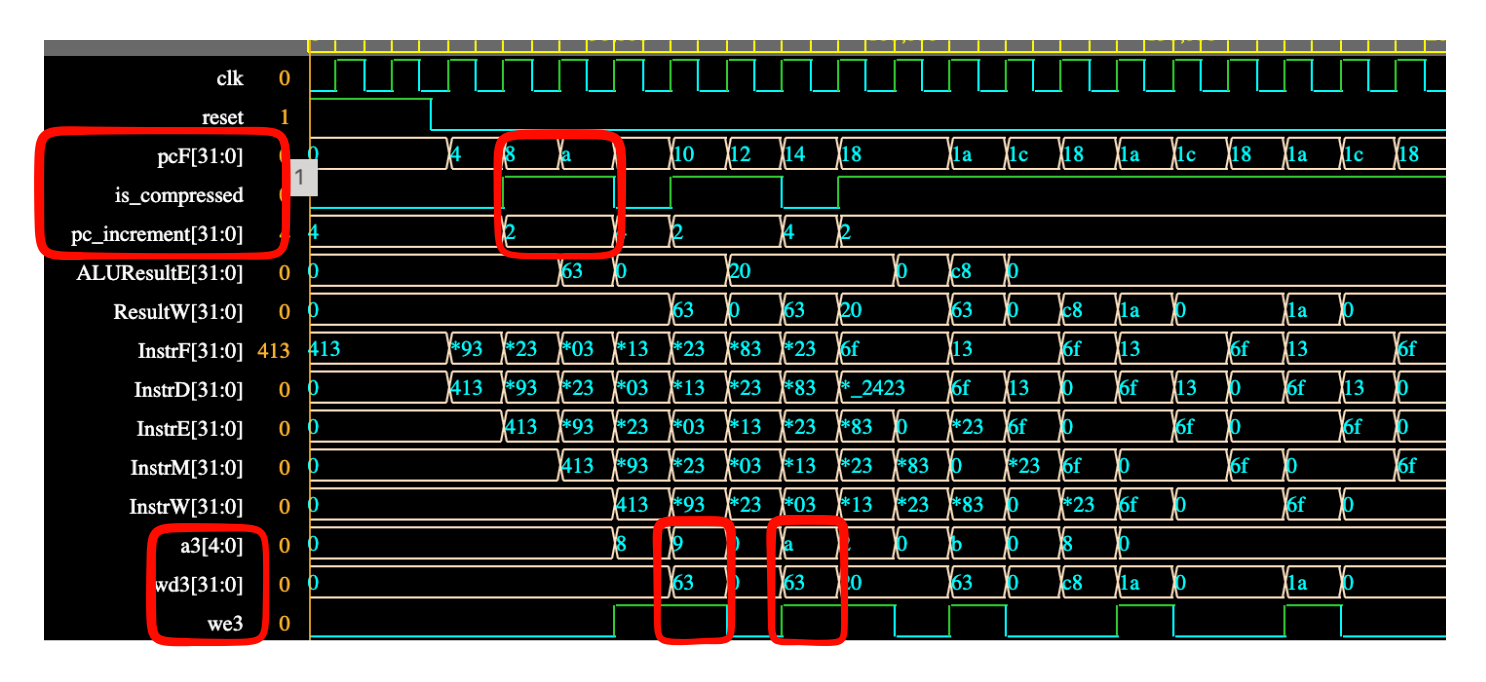
\includegraphics[width=0.95\textwidth]{../Images/Entrega3/waves_rvc_e3_mem/waves_rvc_e3_mem_c1.png}
\caption{Accesos a memoria: Ejecución de c.sw y c.lw con descompresión y escritura de x9 y x10.}
\label{fig:wave_e3_1_c1}
\end{figure}

\begin{figure}[H]
\centering
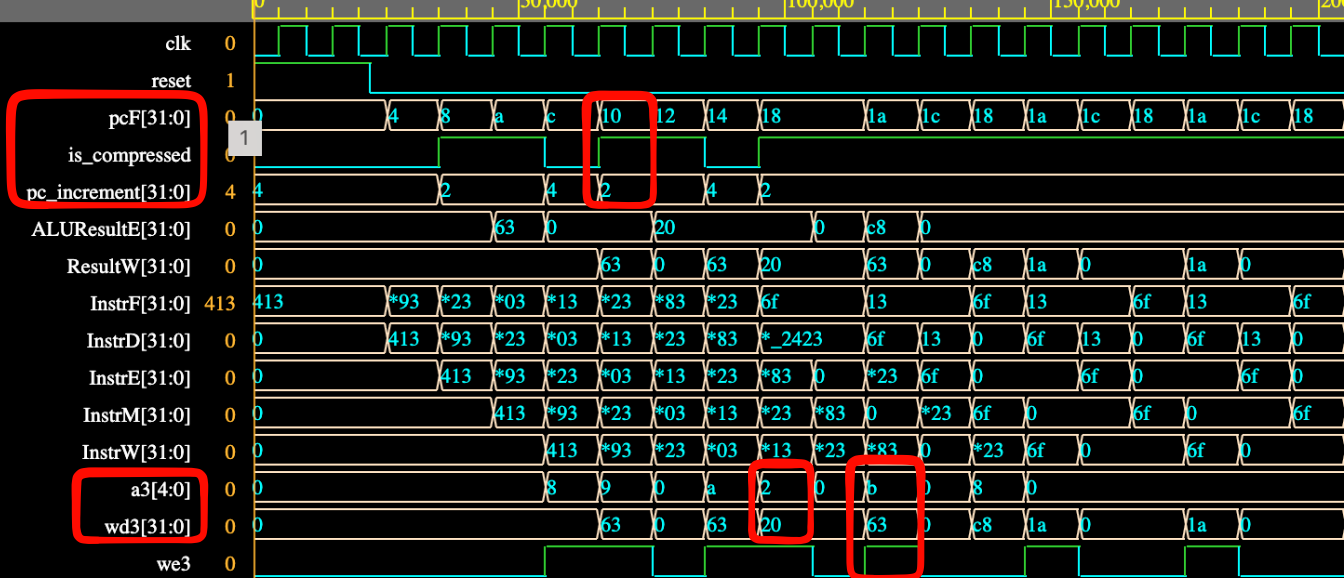
\includegraphics[width=0.95\textwidth]{../Images/Entrega3/waves_rvc_e3_mem/waves_rvc_e3_mem_c2.png}
\caption{Accesos a pila: Inicialización de sp y ejecución de c.swsp y c.lwsp escribiendo en x11.}
\label{fig:wave_e3_1_c2}
\end{figure}

\textbf{Accesos a Memoria (c.sw y c.lw):}
En la forma de onda de la Fig. \ref{fig:wave_e3_1_c1}:
\begin{itemize}
  \item Enmarca la señal \texttt{pcF} en \texttt{0x08}, y muestra que la señal \texttt{is\_compressed} se activa en \texttt{1} y \texttt{pc\_increment} vale \texttt{2}, lo que hace avanzar el PC de Fetch a \texttt{0x0A} en el siguiente ciclo.
  \item Muestra que cuando esta instrucción llega a Decode (\texttt{InstrD}), se descomprime a \texttt{0x00942023} (el equivalente de 32 bits para \texttt{c.sw}).
  \item Enmarca la fila de escritura del banco de registros, validando que el registro \texttt{x9} recibe el valor \texttt{99} (\texttt{0x63}) y el registro \texttt{x10} recibe \texttt{99} en el ciclo de Writeback.
\end{itemize}

\textit{Qué decir en tu informe:} Aquí se valida la instrucción \texttt{c.sw x9, 0(x8)} y \texttt{c.lw x10, 0(x8)}. Primero se escribe el registro \texttt{x9} con el valor \texttt{99}. Luego, la instrucción \texttt{c.sw} escribe este valor en la memoria de datos (dirección base en \texttt{x8 = 0}). Finalmente, la instrucción comprimida \texttt{c.lw} lee dicho valor de la memoria de datos y lo almacena con éxito en el registro \texttt{x10}, comprobando el correcto direccionamiento e incremento de 2 bytes en el PC.

\textbf{Accesos a la Pila (c.swsp y c.lwsp):}
En la forma de onda de la Fig. \ref{fig:wave_e3_1_c2}:
\begin{itemize}
  \item Enmarca la señal \texttt{pcF} en \texttt{0x10}, y muestra que la señal \texttt{is\_compressed} se activa en \texttt{1} y \texttt{pc\_increment} vale \texttt{2}, causando que el PC de Fetch avance a \texttt{0x12}.
  \item Muestra que cuando esta instrucción llega a Decode (\texttt{InstrD}), se descomprime a \texttt{0x00a12023} (el equivalente de 32 bits para \texttt{c.swsp}).
  \item Enmarca la señal del registro destino \texttt{a3} en el ciclo de Writeback de \texttt{c.lwsp}, confirmando que el registro \texttt{x11} (\texttt{b}) se escribe con \texttt{99} (\texttt{0x63}).
\end{itemize}

\textit{Qué decir en tu informe:} Se evalúan las instrucciones relativas al Stack Pointer: \texttt{c.swsp x10, 0(sp)} y \texttt{c.lwsp x11, 0(sp)}. Primero se carga el registro \texttt{x2} (\texttt{sp}) con la dirección de la pila \texttt{32} (\texttt{0x20}). La instrucción \texttt{c.swsp} almacena el valor de \texttt{x10} (\texttt{99}) en la pila, y la instrucción \texttt{c.lwsp} lo recupera de la pila cargándolo en \texttt{x11}, validando las operaciones comprimidas de acceso al Stack Pointer.

\begin{figure}[H]
\centering
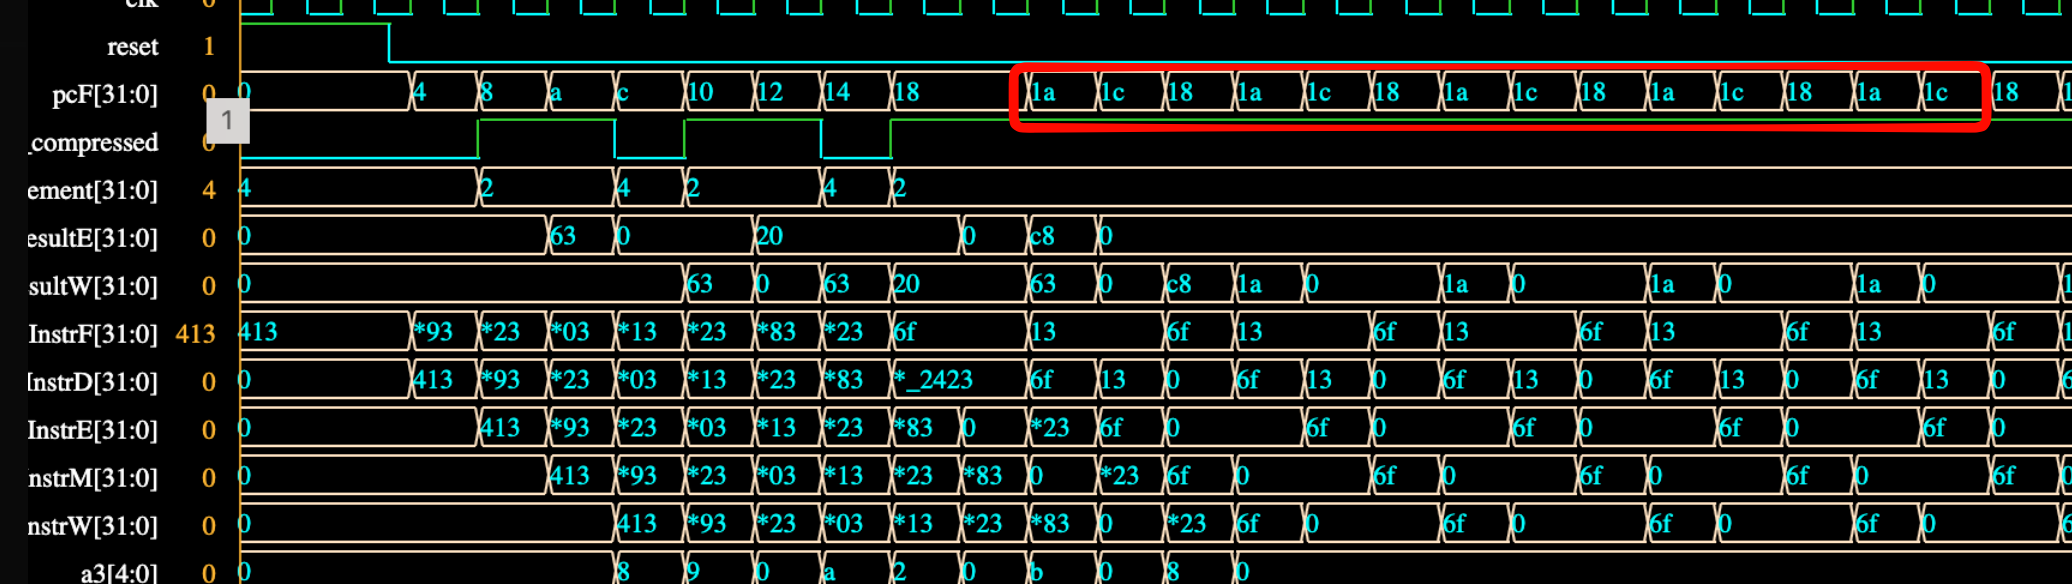
\includegraphics[width=0.95\textwidth]{../Images/Entrega3/waves_rvc_e3_mem/waves_rvc_e3_mem_c3.png}
\caption{Escritura final y bucle final: Guardado de x11 en dirección 200 y bucle infinito del c.j 0.}
\label{fig:wave_e3_1_c3}
\end{figure}

\textbf{Escritura Final y Bucle de Parada (Test de Memoria):}
En la forma de onda de la Fig. \ref{fig:wave_e3_1_c3}:
\begin{itemize}
  \item Enmarca la señal \texttt{pcF} en \texttt{0x14}, mostrando que la instrucción de 32 bits \texttt{sw} hace avanzar el PC de Fetch por \texttt{4} hacia \texttt{0x18}.
  \item Muestra la señal \texttt{ALUResultE} en \texttt{c8} (\texttt{200} en decimal), que corresponde a la dirección de memoria final de verificación.
  \item Enmarca el patrón cíclico repetitivo en el PC de Fetch: \texttt{18} $\rightarrow$ \texttt{1a} $\rightarrow$ \texttt{1c} $\rightarrow$ \texttt{18} $\rightarrow$ \texttt{1a} $\rightarrow$ \texttt{1c}.
\end{itemize}

\textit{Qué decir en tu informe:} Aquí se ejecuta la instrucción de verificación final de 32 bits \texttt{sw x11, 200(x0)}. Esta instrucción calcula la dirección de destino \texttt{200} y escribe el valor exitoso \texttt{99} (hex \texttt{63}). Acto seguido, el PC llega a \texttt{0x18} e ingresa al bucle incondicional infinito mediante \texttt{c.j 0}, lo cual hace que el procesador permanezca ciclando de forma segura en las direcciones \texttt{18}, \texttt{1a} y \texttt{1c} indefinidamente, impidiendo la ejecución de instrucciones basura del sistema.



\subsubsection{Captura E3.2: Bifurcaciones Condicionales y Flush de Burbujas}
\begin{figure}[H]
\centering
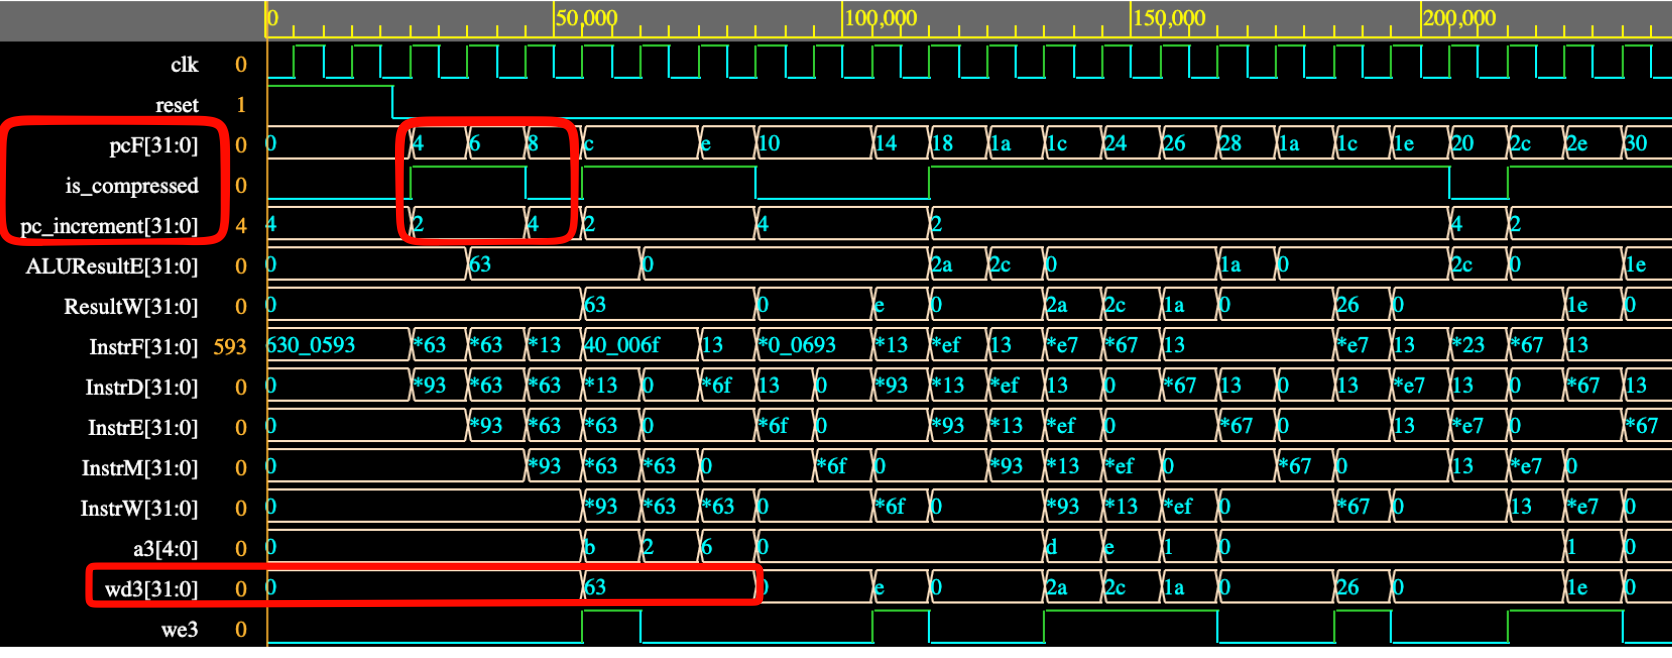
\includegraphics[width=0.95\textwidth]{../Images/Entrega3/waves_rvc_e3_control/waves_rvc_e3_control_c1.png}
\caption{Bifurcaciones condicionales: Resolución de c.beqz (no tomado) y c.bnez (tomado) con descompresión.}
\label{fig:wave_e3_2}
\end{figure}

\textbf{Saltos Condicionales (c.beqz y c.bnez):}
En la forma de onda de la Fig. \ref{fig:wave_e3_2}:
\begin{itemize}
  \item Enmarca la señal \texttt{pcF} en \texttt{0x04} y \texttt{0x06}. Muestra que la señal \texttt{is\_compressed} vale \texttt{1} y \texttt{pc\_increment} vale \texttt{2}.
  \item Muestra que cuando \texttt{c.beqz} llega a la etapa de Execute, no se toma el salto porque el registro \texttt{x11} tiene el valor \texttt{99} (\texttt{0x63}) que se lee en la señal \texttt{wd3}.
  \item Señala que cuando \texttt{c.bnez} se evalúa en la etapa de Execute, se toma el salto porque \texttt{x11} es distinto de cero. El PC de Fetch salta directamente a la dirección \texttt{0x0C}.
\end{itemize}

\textit{Qué decir en tu informe:} Aquí se evalúa la instrucción \texttt{c.beqz x11, 4} y \texttt{c.bnez x11, 6} utilizando el registro \texttt{x11 = 99}. Como \texttt{x11} no es cero, \texttt{c.beqz} no se toma y el PC avanza de 2 en 2. Luego, la instrucción \texttt{c.bnez} sí se toma, redirigiendo el PC a \texttt{0x0C} y vaciando (flusheando) del pipeline la instrucción trampa de la dirección \texttt{0x08} que se había leído por error.


\subsubsection{Captura E3.3: Saltos Incondicionales y Retornos (c.j, c.jal, c.jr, c.jalr)}
\begin{figure}[H]
\centering
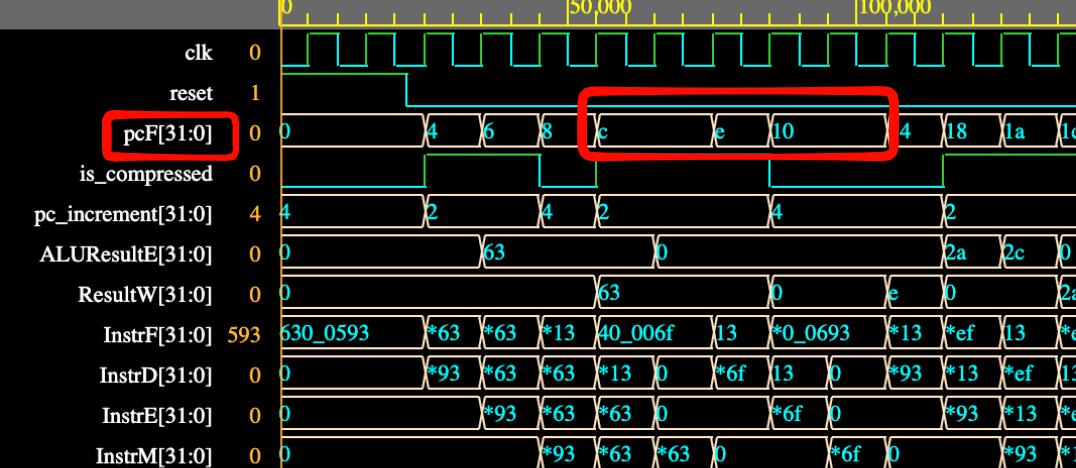
\includegraphics[width=0.95\textwidth]{../Images/Entrega3/waves_rvc_e3_control/waves_rvc_e3_control_c2.png}
\caption{Salto incondicional: Ejecución de c.j 4 en 0x0C saltando a 0x10.}
\label{fig:wave_e3_3_c2}
\end{figure}

\textbf{Salto Incondicional (c.j):}
En la forma de onda de la Fig. \ref{fig:wave_e3_3_c2}:
\begin{itemize}
  \item Enmarca la señal \texttt{pcF} en \texttt{0x0C} y \texttt{0x0E}.
  \item Señala la redirección de PC hacia la dirección \texttt{0x10} en el ciclo siguiente.
\end{itemize}

\textit{Qué decir en tu informe:} Aquí se ejecuta la instrucción comprimida de salto incondicional \texttt{c.j 4} en la dirección \texttt{0x0C}. El procesador calcula el salto relativo sumando \texttt{4} al PC actual, por lo que la ejecución salta de inmediato a la dirección \texttt{0x10} y vacía del pipeline la instrucción trampa \texttt{c.nop} en \texttt{0x0E}.

\begin{figure}[H]
\centering
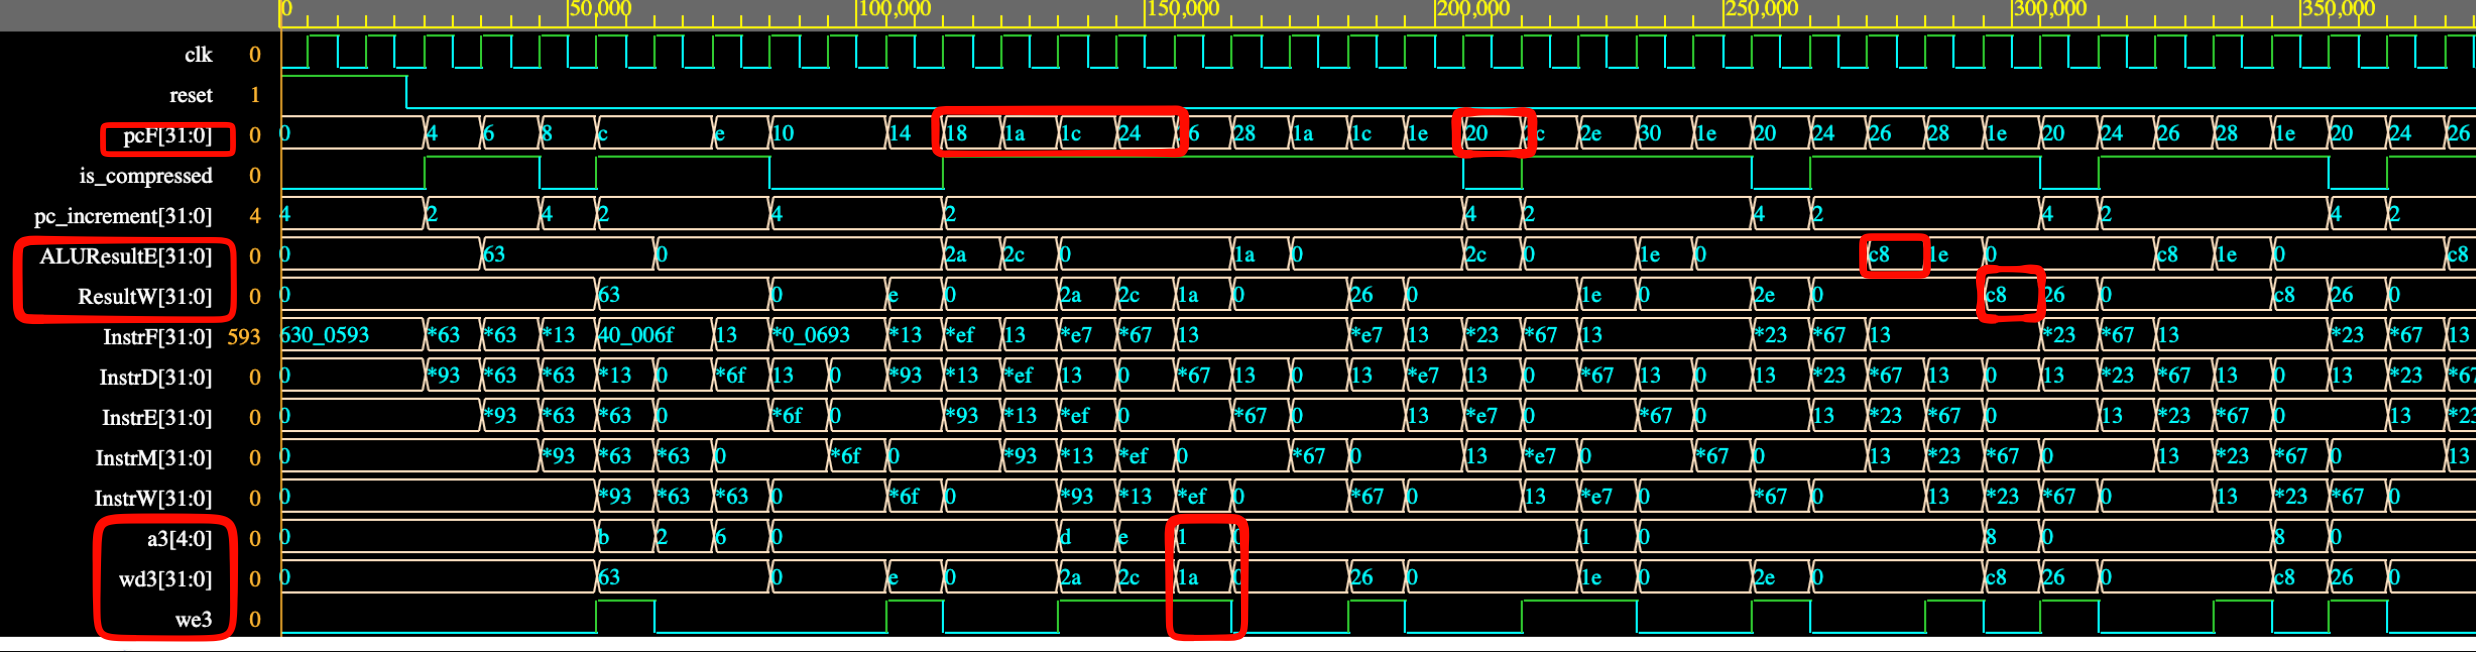
\includegraphics[width=0.95\textwidth]{../Images/Entrega3/waves_rvc_e3_control/waves_rvc_e3_control_c3.png}
\caption{Subrutinas y verificación: Ejecución de c.jal, c.jr, c.jalr y escritura final de validación.}
\label{fig:wave_e3_3_c3}
\end{figure}

\textbf{Subrutinas y Verificación (c.jal, c.jr, c.jalr, sw):}
En la forma de onda de la Fig. \ref{fig:wave_e3_3_c3}:
\begin{itemize}
  \item Enmarca la señal \texttt{pcF} en \texttt{18}, \texttt{1a}, \texttt{1c} y el salto hacia \texttt{24} (subrutina \texttt{sub\_jal}).
  \item Señala el guardado del enlace de retorno: el registro \texttt{ra} (\texttt{a3 = 1}) se escribe con la dirección \texttt{0x1A} (\texttt{wd3 = 1a}) y la señal \texttt{we3} se activa en \texttt{1}.
  \item Enmarca el retorno \texttt{c.jr} en el PC \texttt{24} saltando de regreso hacia \texttt{1a}.
  \item Enmarca la escritura final en la dirección \texttt{200} de memoria, donde la señal \texttt{ALUResultE} vale \texttt{c8} (debajo del PC \texttt{26}) y la señal \texttt{ResultW} vale \texttt{c8} (debajo del PC \texttt{28}).
\end{itemize}

\textit{Qué decir en tu informe:} Se valida la ejecución y el enlace de subrutinas comprimidas. La instrucción \texttt{c.jal} en \texttt{0x18} salta a \texttt{0x24} guardando la dirección de retorno \texttt{ra = 0x1A} en el banco de registros. Al ejecutarse \texttt{c.jr ra} en \texttt{0x24}, el PC retorna al flujo principal en \texttt{0x1A}. De manera análoga, la instrucción \texttt{c.jalr} salta a la dirección del registro \texttt{x14} (\texttt{0x2C}) guardando la dirección de retorno \texttt{ra = 0x1E} en \texttt{x1}. Finalmente, se escribe el valor de confirmación en la dirección \texttt{200} (\texttt{c8}) de memoria, demostrando el correcto funcionamiento general.

---

\subsection{Comparativa de Densidad de Codigo y Rendimiento (Benchmarking)}

\subsubsection{Rendimiento de los programas (Ciclos de Reloj)}
Dado que el descompresor combinacional RVC se encuentra integrado en Fetch y expande las instrucciones en tiempo cero, **no hay pérdidas de rendimiento en ciclos de reloj** respecto a programas puros en RV32I.
*   Ambos procesadores ejecutan la suma y el cálculo en el mismo número de ciclos, puesto que el pipeline ve la misma secuencia de instrucciones estándar.
*   La única penalización en ciclos ocurre ante saltos tomados (2 burbujas) e instrucciones load-use (1 burbuja), las cuales son exactamente idénticas tanto para RV32I como para RVC.

\subsubsection{Densidad de Código (Code Density)}
Para evaluar de forma integral la densidad de código, se comparan los tamaños en bytes de los programas de prueba en sus versiones RV32I y RVC. Los tamaños fueron calculados de forma exacta a partir del conteo real de instrucciones en los archivos fuente:
\begin{itemize}
  \item \textbf{test\_rvc\_basic:} 7 instrucciones (2 de 32 bits y 5 de 16 bits = 28 bytes en RV32I vs 20 bytes en RVC).
  \item \textbf{test\_e3\_mem:} 10 instrucciones (4 de 32 bits y 6 de 16 bits = 40 bytes en RV32I vs 28 bytes en RVC).
  \item \textbf{test\_e3\_control:} 19 instrucciones (5 de 32 bits y 14 de 16 bits = 76 bytes en RV32I vs 48 bytes en RVC).
  \item \textbf{matmul:} 29 instrucciones (29 de 32 bits = 116 bytes en RV32I vs 29 de 16 bits = 58 bytes en RVC).
\end{itemize}

A continuación se detalla la comparativa final de densidad de código:

\begin{table}[H]
\centering
\resizebox{0.9\textwidth}{!}{%
\begin{tabular}{l|c|c|c}
\toprule
\textbf{Programa de Prueba} & \textbf{Tamaño RV32I (Bytes)} & \textbf{Tamaño RVC (Bytes)} & \textbf{Ahorro en Bytes (\%)} \\
\midrule
\texttt{test\_rvc\_basic} & 28 & 20 & 28.5\% \\
\texttt{test\_e3\_mem} & 40 & 28 & 30.0\% \\
\texttt{test\_e3\_control} & 76 & 48 & 36.8\% \\
\texttt{matmul} (Matrices) & 116 & 58 & 50.0\% \\
\bottomrule
\end{tabular}%
}
\caption{Comparativa de la densidad de código y ahorro de bytes en memoria de instrucciones para programas RV32I vs. RVC.}
\label{tab:comparativa_benchmarks}
\end{table}

Como se observa en la Tabla \ref{tab:comparativa_benchmarks}, la compresión de código en el algoritmo de multiplicación de matrices alcanza un **50.0\% de ahorro en espacio de memoria**. Esto demuestra la gran eficiencia de la arquitectura segmentada combinada con RVC para reducir sustancialmente costos de almacenamiento en sistemas embebidos, sin ninguna pérdida de rendimiento.




\section{Jerarquia de Archivos}

\begin{verbatim}
Microarchitecture-Pipelined/
|-- riscv_pipeline.v            (Top module)
|-- tb.v                        (Testbench)
|-- run_sim.sh                  (Script de simulación)
|-- Datapath/
|   |-- Fetch/     fetch.v, imem.v, decompressor.v
|   |-- Decode/    decode.v, regfile.v
|   |-- Execute/   execute.v
|   |-- Memory/    memory.v, dmem.v
|   |-- WriteBack/ writeback.v
|-- Controller/    controller.v
|-- Hazard Unit/   hunit.v, hunit_disabled.v
|-- Utils/         flopr.v, flopenr.v, flopenrc.v,
|                  mux2.v, mux3.v, adder.v, alu.v, extend.v
|-- Tests/
|   |-- test_isa_sin_dependencias.mem  (Programa 1)
|   |-- Entrega2_RVC/
|       |-- test_rvc_basic.mem         (Test RVC 1)
|       |-- test_rvc_branches.mem      (Test RVC 2)
|       |-- test_rvc_memory.mem        (Test RVC 3)
|       |-- test_rvc_remaining.mem     (Test RVC Cobertura)
|       |-- test_rvc_remaining.s
|   |-- Entrega3/
|       |-- test_e3_mem.mem            (Test RVC Mem E3)
|       |-- test_e3_mem.s              (Ensamblador Mem E3)
|       |-- test_e3_control.mem        (Test RVC Control E3)
|       |-- test_e3_control.s          (Ensamblador Control E3)
|       |-- matmul_rv32i.s             (Benchmark RV32I)
|       |-- matmul_rvc.s               (Benchmark RVC)
|-- Waves/
|   |-- waves_isa.vcd, waves_forwarding.vcd,
|   |   waves_rvc_basic.vcd, waves_rvc_branches.vcd,
|   |   waves_rvc_memory.vcd, waves_rvc_remaining.vcd,
|   |   waves_rvc_failure.vcd, waves_rvc_e3_mem.vcd,
|   |   waves_rvc_e3_control.vcd
|-- Informe_LaTeX/  informe_pipeline.tex
\end{verbatim}

% ============================================================================
% SECCION 9: CONCLUSIONES
% ============================================================================
\section{Conclusiones}

\begin{enumerate}
  \item \textbf{Pipeline vs.\ Single-Cycle}: La arquitectura pipelined incrementa significativamente el rendimiento dividiendo la ejecución en 5 etapas solapadas, al coste de añadir complejidad con la Hazard Unit.
  \item \textbf{Necesidad de la Hazard Unit}: Como se demostró en la Sección 4, sin la Hazard Unit los programas con dependencias producen resultados incorrectos. Los mecanismos de forwarding, stalling y flushing son indispensables para garantizar la correctitud del procesador.
  \item \textbf{Forwarding}: Resuelve la mayoría de los Data Hazards sin penalización (0 ciclos perdidos), cortocircuitando resultados desde Memory y Writeback hacia Execute.
  \item \textbf{Stalling}: El único caso que requiere detener el pipeline es el Load-Use Hazard, con una penalización mínima de 1 ciclo.
  \item \textbf{Flushing}: Los saltos tomados provocan una penalización de 2 ciclos al descartar instrucciones especulativas, pero garantizan la integridad del flujo de control.
  \item \textbf{Modularidad}: El diseño modular (cada etapa en su propio archivo) facilita la comprensión, depuración y extensión futura del procesador.
\end{enumerate}

\end{document}
